%!TEX TS-program = xelatex
%!TEX encoding = UTF-8

% To be compiled by XeLaTeX, preferably under TeX Live.
% LaTeX source for ``Yanqi Lake Lectures on Algebra'' Part III.
% Copyright 2019  李文威 (Wen-Wei Li).
% Permission is granted to copy, distribute and/or modify this
% document under the terms of the Creative Commons
% Attribution-NonCommercial 4.0 International (CC BY-NC 4.0)
% https://creativecommons.org/licenses/by-nc/4.0/

% The document is based on the standard book class.
\documentclass[a4paper,12pt]{book}
\usepackage[backend=biber, hyperref=auto, backref=true]{biblatex}

\usepackage{amsmath}
\usepackage{amsthm}
\usepackage{amssymb}

% Indexing via imakeidx + xindy
\usepackage[xindy]{imakeidx}
\makeindex[columns=2, program=truexindy, intoc=true, options=-M texindy -I xelatex -C utf8, title={Index}]

% Hyperref set-up
\usepackage[unicode, colorlinks]{hyperref}
\hypersetup{
	linkcolor = blue,
	citecolor = red,
	urlcolor = teal,
	bookmarksnumbered = true,
	pdfauthor = {Wen-Wei Li},
	pdftitle = {Yanqi Lake Lectures on Algebra: Part 3}
}

% Overall font set-up
\usepackage{fontspec}
\usepackage{unicode-math}
\setromanfont{TeX Gyre Pagella}
\setsansfont{TeX Gyre Heros Cn}
\setmathfont[math-style=ISO, bold-style=ISO]{texgyrepagella-math.otf}

% Make \today print yyyy-mm-dd
\usepackage[iso, english]{isodate}

\def\CoverPage{Cover-page.pdf}	% Cover page to be included (here: a PDF file)


% Change the geometry if need be
\usepackage{geometry}
\geometry{
	paper=a4paper,
	top=3cm,
	inner=2.54cm,
	outer=2.54cm,
	bottom=3cm,
	headheight=6ex,
	headsep=6ex,
}

\usepackage{stmaryrd}
\usepackage{bbding}
\usepackage[nottoc]{tocbibind}
\usepackage{mathrsfs}
\usepackage[centercolon]{mathtools}
\usepackage[dvipsnames]{xcolor}
\usepackage{tikz-cd}
\usetikzlibrary{positioning, shapes.geometric, patterns, matrix, knots}

\usepackage{paralist}
\usepackage[figurewithin=none]{caption}
\usepackage{graphicx}

% Environments for theorems etc.
% I prefer linear ordering within sections.
\theoremstyle{plain}
\newtheorem{proposition}{Proposition}[section]
\newtheorem{lemma}[proposition]{Lemma}
\newtheorem{theorem}[proposition]{Theorem}
\newtheorem{corollary}[proposition]{Corollary}
\newtheorem{fact}[proposition]{Fact}
\theoremstyle{definition}
\newtheorem{definition}[proposition]{Definition}
\newtheorem{definition-theorem}[proposition]{Definition-Theorem}
\newtheorem{definition-proposition}[proposition]{Definition-Proposition}
\newtheorem{hypothesis}[proposition]{Hypothesis}
\newtheorem{example}[proposition]{Example}
\newtheorem{exercise}[proposition]{Exercise}
\theoremstyle{remark}
\newtheorem{remark}[proposition]{Remark}
\newtheorem{note}[proposition]{Note}
\newtheorem{notation}[proposition]{Notation}
\newtheorem{convention}[proposition]{Convention}
\newtheorem{conjecture}[proposition]{Conjecture}

% Customize the numbering of equations
\numberwithin{equation}{chapter}
\renewcommand{\theequation}{\thechapter--\arabic{equation}}

% Use the usual symbols for real and imaginary parts of a complex number
\renewcommand{\Re}{\operatorname{Re}}
\renewcommand{\Im}{\operatorname{Im}}

\renewcommand*\arraystretch{1.5} % Extra spacing in a table environment.

% Load custom commands
\usepackage{mycommand}
\usepackage{myarrows}

\usepackage{xstring}
\usepackage{pdfpages}

\usepackage{fancyhdr}
\newcommand\sectionname{\arabic{chapter}.\arabic{section}}
\pagestyle{fancy}
	\renewcommand{\chaptermark}[1]{\markboth{\scshape #1}{}}
	\renewcommand{\sectionmark}[1]{\markright{\S\sectionname\quad \scshape #1}}
	\fancyhf{} % delete current setting for header and footer
	\fancyhead[EC]{\footnotesize{\leftmark}\vspace{1mm}}
	\fancyhead[OC]{\footnotesize{\rightmark}\vspace{1mm}}
	\fancyhead[LE,RO]{$\cdot\;${\footnotesize \thepage}$\;\cdot$\vspace{1mm}} %
	\fancyhead[RE,LO]{}
	\renewcommand{\headrulewidth}{0.5pt}
	\renewcommand{\footrulewidth}{0pt}
	\addtolength{\headheight}{0.5pt}

\fancypagestyle{plain}{%
	\fancyhead{} % get rid of headers on plain pages
	\renewcommand{\headrulewidth}{0pt} % and the line
}

% Set up the chapter titles
\usepackage{titlesec}
\titleformat{\chapter}[display]
	{\filleft\normalfont\fontspec[Scale=2.5]{League Spartan}}
	{Lecture \thechapter}
	{10mm}
	{}[]

% Customize biblatex
\DeclareFieldFormat{postnote}{#1}	% Disable pagination in postnote for biblatex
\addbibresource{YAlg3.bib}

\begin{document}
	\frontmatter
	% Make the cover page by reading the file \CoverPage if it exists.
	\ifdefempty{\CoverPage}{%
		\relax
	}{%
		\pagestyle{empty}%	Clean-up the page style
		\renewcommand{\thepage}{C\arabic{page}}%	The page numbers here should start with "C" (PDF: logical page numbers)
		\IfEndWith{\CoverPage}{.pdf}{% If the file name ends with .pdf or .PDF, we include the PDF file directly.
			\includepdf{\CoverPage}
		}{%
			\IfEndWith{\CoverPage}{.PDF}{%
				\includepdf{\CoverPage}
			}{%
				\input{\CoverPage}		% Otherwise we import the TeX source
			}
		}%
		\pagestyle{fancy}		% Resume the page style to "fancy".
		\pagenumbering{roman}	% Resume the page numbers to roman style.
	}
	
	\begin{titlepage}
		\vspace*{\stretch{1}}
		\noindent\begin{center}\rule{\linewidth}{2pt}\end{center}	% Draw a rule
		\begin{center}
			\Huge \textbf{Yanqi Lake Lectures on Algebra}  \\ \vspace{1em}
			\Huge Part 3
		\end{center}
		\noindent\begin{center}\rule{\linewidth}{2pt}\end{center}	% Draw a rule
		\vspace{1em}
		\begin{center}
			{\Large Wen-Wei Li} \\ \vspace{1em}
			{\Large Chinese Academy of Sciences} \\ \vspace{1.5em}
		\end{center}
		\vfill
%		\begin{center} \href{http://www.ucas.edu.cn}{\includegraphics[height=40pt]{logo-UCAS.png}} \end{center}
	\end{titlepage}
	
	\newpage
	\thispagestyle{empty}
	\begin{center}
		\Large Version: \today
	\end{center}
	\vfill
	\begin{tabular}{p{.9\textwidth}}
		The cover page uses the fonts \textit{Bebas Neue} and \textit{League Gothique}, both licensed under the \href{https://opensource.org/licenses/OFL-1.1}{SIL Open Font License}. \\  \vspace{\baselineskip}
		This work is licensed under a Creative Commons Attribution-NonCommercial 4.0 International License. To view a copy of this license, visit \url{http://creativecommons.org/licenses/by-nc/4.0/}. \\
		\vspace{\baselineskip}
		\begin{center}
			\includegraphics[scale=1]{by-nc.eps}
		\end{center}\\
	\end{tabular}

	\tableofcontents

	\mainmatter
	% To be compiled by XeLaTeX, preferably under TeX Live.
% LaTeX source for ``Yanqi Lake Lectures on Algebra'' Part III.
% Copyright 2019  李文威 (Wen-Wei Li).
% Permission is granted to copy, distribute and/or modify this
% document under the terms of the Creative Commons
% Attribution-NonCommercial 4.0 International (CC BY-NC 4.0)
% https://creativecommons.org/licenses/by-nc/4.0/

% To be included
\chapter*{Introduction}
\addcontentsline{toc}{chapter}{Introduction}
\markboth{Introduction}{}

In the beginning, these lecture notes were prepared for the graduate course \emph{Algebra III} (ID: 011M4002Y) in Spring 2016, University of the Chinese Academy of Sciences. For some reasons, it took place in the Yuquanlu campus instead of the Yanqi Lake campus as it should be.

The course is a sequel to Algebra I (fields, modules and representations) and II (homological algebra). The topic of this Part III is commutative algebra, or more precisely \emph{commutative ring theory}. Each ``Lecture'' in these notes took roughly one week, say approximately four hours of lecture, but the materials were only partially covered. My initial intention was to give a traditional course on commutative algebra as proposed by the syllabus prescribed by UCAS. For various reasons, my plan failed. For example, there are too few discussions on depth, regular sequences and Cohen--Macaulay modules, too few applications of completions, and the computational aspects haven't been touched. Moreover, the homological aspect of commutative algebra is almost non-existent in these notes, namely the Auslander--Buchsbaum Formula, the properties of regular local rings, etc. Last but not least, the exercises herein are scarcely sufficient.

These notes were also used for the Enhanced Program for Graduate Study held at the Beijing International Center of Mathematical Research, Peking University, during Spring 2019 (course ID: 00102057).

As the title suggests, some backgrounds from the Part I are presumed, namely the basic notions of rings, modules and their chain conditions, as well as familiarity with tensor products and some Galois theory. We occasionally presume some basic knowledge of homological algebra, such as the functors $\Tor_i$ and $\Ext^i$.

Sometimes I made free use of the language of derived categories. This was indeed covered in the preceding course \emph{Algebra II}, and it should be common sense for the future generations.

As the reader might have observed, these notes were prepared in a rush; certain paragraphs have not been proofread yet and many proofs are silly. I am very grateful to the students for various corrections and improvements, and I will try to polish these notes in the future.

\section*{Conventions}
Throughout these lectures, we consider only associative rings with unit $1$, and the rings and algebras are assumed to be commutative and nonzero unless otherwise specified. The ideal generated by elements $x_1, x_2, \ldots$ in a ring $R$ is denoted by $(x_1, x_2, \ldots)$ or sometimes $\langle x_1, x_2, \ldots \rangle$; the $R$-algebra of polynomials in variables $X, Y, \ldots$ with coefficients in $R$ is denoted by $R[X, Y, \ldots]$. We write $R^\times$ for the group of invertible elements in a ring $R$. A ring without zero-divisors except $0$ is called an integral domain, or simply a domain. The localization of a ring $R$ with respect to a multiplicative subset $S$ will be written as $R[S^{-1}]$.

For any sets $E, F$, let $E \smallsetminus F := \left\{ x \in E: x \notin F \right\}$. The cardinality of $E$ is denoted by $|E|$.

The usual logical connectives such as $\exists$, $\forall$, $\wedge$, $\vee$ and so forth will occasionally be used. Writing $A := B$ means that the expression $A$ is defined to be $B$.

We will use the standard notations $\Z, \Q, \R, \CC$ to denote the set of integers, of rational numbers, etc. Sans serif fonts are reserved for categories, such as $\cate{Ab}$ (abelian groups) and $\cate{Ring}$. 

When denoting morphisms in a category by arrows, monomorphisms (resp.\ epimorphisms, isomorphisms) will be indicated $\hookrightarrow$ (resp.\ $\twoheadrightarrow, \rightiso$).

\section*{Possible references}
The reader is expected to have basic familiarity with groups, rings and modules, as covered in my lecture notes on Algebra I. We will make use of some really elementary homological algebra as our course proceeds --- so keep calm.

Our main references will be \cite{Mat80} and \cite{Eis95}. The Bourbaki volumes \cite{Bour83, Bour98} serve as our ultimate source. The readers are also encouraged to consult the relevant materials in \href{https://stacks.math.columbia.edu/}{Stacks Project}.

\vfill
\begin{figure}[h]
	\centering 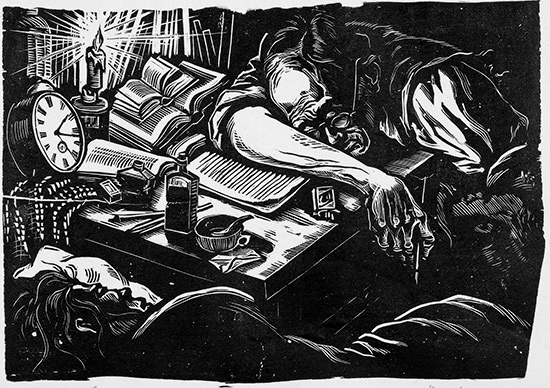
\includegraphics[height=180pt]{JiaoShouShengYa.jpg} \\ \vspace{1em}
	\begin{minipage}{0.7\textwidth}\begin{center}
		\small \fontspec{Noto Serif CJK SC} 《教授生涯》, 李桦, 木刻版画, 1948 年.
	\end{center}\end{minipage}
\end{figure}
\vfill
	% To be compiled by XeLaTeX, preferably under TeX Live.
% LaTeX source for ``Yanqi Lake Lectures on Algebra'' Part III.
% Copyright 2019  李文威 (Wen-Wei Li).
% Permission is granted to copy, distribute and/or modify this
% document under the terms of the Creative Commons
% Attribution-NonCommercial 4.0 International (CC BY-NC 4.0)
% https://creativecommons.org/licenses/by-nc/4.0/

% To be included
\chapter{Warming up}

The reader might be familiar with most of the materials in this lecture. Our goal is to fix notation and present the basic structural results on Noetherian and Artinian rings or modules, including the celebrated Nakayama's Lemma which will be used repeatedly.

\section{Review on ring theory}
Let $R$ be a ring, supposed to be commutative with unit $1 \neq 0$ as customary. Recall that an ideal $I \subsetneq R$ is called
\begin{compactitem}
	\item \emph{prime}, if $ab \in I \iff (a \in I) \vee (b \in I)$;
	\item \emph{maximal}, if $I$ is maximal among the proper ideals of $R$ with respect to inclusion.
\end{compactitem}
Recall the following standard facts
\begin{itemize}
	\item $I$ is prime if and only if $R/I$ is an integral domain, i.e. has no zero divisors except $0$;
	\item $I$ is maximal if and only if $R/I$ is a field; in particular, maximal ideals are prime;
	\item every proper ideal $I$ is contained in a maximal ideal (an application of Zorn's Lemma).\index{Zorn's Lemma}
\end{itemize}

\begin{definition}[Local rings] \index{local ring}
	The ring $R$ is called \emph{local} if it has a unique maximal ideal, \emph{semi-local} if it has only finitely many maximal ideals.
	
	Let $\mathfrak{m}$ be the maximal ideal of a local ring $R$. We call $R/\mathfrak{m}$ the \emph{residue field} of $R$. A local homomorphism between local rings $\varphi: R_1 \to R_2$ is a ring homomorphism such that $\varphi(\mathfrak{m}_1) \subset \mathfrak{m}_2$. Consequently, local homomorphisms induce embeddings on the level of residue fields.
\end{definition}
Sometimes we denote a local ring by the pair $(R, \mathfrak{m})$.

\begin{remark}
	Let $R$ be a local ring with maximal ideal $\mathfrak{m}$, then $R^\times = R \smallsetminus \mathfrak{m}$. The is easily seen as follows. An element $x \in R$ is invertible if and only if $Rx = R$. Note that $Rx=R$ is equivalent to that $x$ is not contained in any maximal ideal, and the only maximal ideal is $\mathfrak{m}$.
\end{remark}

Throughout these lectures, we shall write \index{Spec@$\Spec(R)$} \index{MaxSpec@$\MaxSpec(R)$}
\begin{align*}
	\Spec(R) & := \{ \text{prime ideals of } R \}, \\
	\MaxSpec(R) & := \{ \text{maximal ideals of } R \}.
\end{align*}
They are called the \emph{spectrum} and the \emph{maximal spectrum} of $R$, respectively. The upshot is that $\Spec(R)$ comes with a natural topology.

\begin{definition}[Zariski topology] \index{Zariski topology}\index{$V(\mathfrak{a})$}
	For any ideal $\mathfrak{a} \subset R$, set $V(\mathfrak{a}) := \{ \mathfrak{p} \in \Spec(R): \mathfrak{p} \supset \mathfrak{a} \}$. Then there is a topology on $\Spec(R)$, called the \emph{Zariski topology}, whose closed subset are precisely $V(\mathfrak{a})$, for various ideals $\mathfrak{a}$.
\end{definition}
Indeed, we only have to prove the family of subsets $\{ V(\mathfrak{a}) : \mathfrak{a} \subset R \}$ is closed under finite union and arbitrary intersections. It boils down to the easy observation that $V(\mathfrak{a}) \cup V(\mathfrak{b}) = V(\mathfrak{a}\mathfrak{b})$ (check this!) and $\bigcap_{\mathfrak{a} \in \mathcal{A}} V(\mathfrak{a}) = V\left( \sum_{\mathfrak{a} \in \mathcal{A}} \mathfrak{a} \right)$, where $\mathcal{A}$ is any family of ideals.

Given a ring homomorphism $\varphi: R_1 \to R_2$, if $I \subset R_2$ is an ideal, then $\varphi^{-1}(I) \subset R_1$ is also an ideal.
\begin{proposition}
	Given $\varphi$ as above, it induces a continuous map
	\begin{align*}
		\varphi^\sharp: \Spec(R_2) & \longrightarrow \Spec(R_1) \\
		\mathfrak{p} & \longmapsto \varphi^{-1}(\mathfrak{p})
	\end{align*}
	with respect to the Zariski topologies on spectra.
\end{proposition}
\begin{proof}
	Clearly, $ab \in \varphi^{-1}(\mathfrak{p})$ is equivalent to $\varphi(a)\varphi(b) \in \mathfrak{p}$, which is in turn equivalent to $(\varphi(a) \in \mathfrak{p}) \vee (\varphi(b) \in \mathfrak{p})$ when $\mathfrak{p}$ is prime.
	
	To show the continuity of $\varphi^\sharp$, observe that for any ideal $\mathfrak{a} \subset R_1$ and $\mathfrak{p} \in \Spec(R_2)$, we have $\varphi^{-1}(\mathfrak{p}) \supset \mathfrak{a}$ if and only if $\mathfrak{p} \supset \varphi(\mathfrak{a})$, i.e. $\mathfrak{p} \in V(\varphi(\mathfrak{a}) R_2)$. Hence the preimage of closed subsets are still closed.
\end{proof}

More operations on spectra:
\begin{itemize}
	\item Take $R_1$ to be a subring of $R_2$ and $\varphi$ be the inclusion map, the map above becomes $\mathfrak{p} \mapsto \mathfrak{p} \cap R_1$.
	\item Take $\varphi: R \twoheadrightarrow R/I$ to be a quotient homomorphism, then $\varphi^{-1}$ is the usual bijection from $\Spec(R/I)$ onto $V(I)$.
	\item In general, $\varphi^{-1}$ does not induce $\MaxSpec(R_2) \to \MaxSpec(R_1)$, as illustrated in the case $\varphi: \Z \hookrightarrow \Q$.
\end{itemize}

At this stage, we can prove a handy result concerning prime ideals.
\begin{proposition}[Prime avoidance]\label{prop:prime-avoidance} \index{prime avoidance}
	Let $I$ and $\mathfrak{p}_1, \ldots, \mathfrak{p}_n$ be ideals of $R$ such that $I \subset \bigcup_{i=1}^n \mathfrak{p}_i$. Suppose that
	\begin{compactitem}
		\item either $R$ contains an infinite field, or
		\item at most two of the ideals $\mathfrak{p}_1, \ldots, \mathfrak{p}_n$ are non-prime,
	\end{compactitem}
	then there exists $1 \leq i \leq n$ such that $I \subset \mathfrak{p}_i$.
\end{proposition}
\begin{proof}
	If $R$ contains an infinite field $F$, the ideals are automatically $F$-vector subspaces of $R$. Since $I = \bigcup_{i=1}^r I \cap \mathfrak{p}_i$ whereas an $F$-vector space cannot be covered by finitely many proper subspaces, there must exist some $i$ with $I \cap \mathfrak{p}_i = I$.

	Under the second assumption, let us argue by induction on $n$ that $\forall i \; I \not\subset \mathfrak{p}_i$ implies $I \not\subset \bigcup_{i=1}^n \mathfrak{p}_i$. The case $n=1$ is trivial. When $n \geq 2$, by induction we may choose, for each $i$, an element $x_i \in I \smallsetminus \bigcup_{j \neq i} \mathfrak{p}_j$. Suppose on the contrary that $I \subset \bigcup_{j=1}^n \mathfrak{p}_j$, then we would have $x_i \in \mathfrak{p}_i$, for all $i=1, \ldots, n$.

	When $n=2$ we have $x_1 + x_2 \notin \mathfrak{p}_1 \cup \mathfrak{p}_2$ and $x_1 + x_2 \in I$, a contradiction. When $n > 2$, we may assume $\mathfrak{p}_1$ is prime, therefore
	\[ x_1 + \prod_{j=2}^n x_j \notin \bigcup_{i=1}^n \mathfrak{p}_i, \]
	again a contradiction.
\end{proof}

\begin{exercise}
	The following construction from \cite[Exercise 3.17]{Eis95} shows that the assumptions of Proposition \ref{prop:prime-avoidance} cannot be weakened. Take $R = (\Z/2\Z)[X, Y] / (X,Y)^2$, which has a basis $\{1, X, Y\}$ (modulo $(X,Y)^2$) as a $\Z/2\Z$-vector space. Show that the image $\mathfrak{m}$ of $(X, Y)$ in $R$ is the unique prime ideal, and can be expressed as a union of three ideals properly contained in $\mathfrak{m}$.
\end{exercise}

\section{Localization of rings and modules} \index{localization}\index{$M[S^{-1}]$}
Let $S$ be a \emph{multiplicative subset} of $R$, which means that
\begin{inparaenum}[(a)]\index{multiplicative subset}
	\item $1 \in S$,
	\item $S$ is closed under multiplication, and
	\item $0 \notin S$.
\end{inparaenum}
The \emph{localization} of $R$ with respect to $S$ is the ring $R[S^{-1}]$ formed by classes $[r,s]$ with $r \in R$, $s \in S$, modulo the equivalence relation
\[ [r,s] = [r',s'] \iff \exists t \in S, \; (rs' - r's)t = 0. \]

You should regard $[r,s]$ as a token for $r/s$; the ring structure of $R[S^{-1}]$ is therefore evident. In brief, localization amounts to formally inverting the elements of $S$, whence the notation $R[S^{-1}]$. Note that condition (c) guarantees $R[S^{-1}] \neq \{0\}$.

\begin{exercise}
	Given $R$ and $S$, show that $r \mapsto r/1$ yields a natural homomorphism $R \to R[S^{-1}]$ and show that its kernel equals $\{r: \exists s \in S, \; sr=0 \}$.
\end{exercise}

The universal property of $R \to R[S^{-1}]$ can be stated using commutative diagrams as follows.
\[
	\forall \left\{ \begin{array}{l}
		\varphi: R \to R': \; \text{ring homomorphism} \\
		\text{s.t. } \varphi(S) \subset (R')^\times
	\end{array}\right. ,\quad
	\begin{tikzcd}
		R \arrow[r] \arrow[rd, "\varphi"'] & R[S^{-1}] \arrow[d, dashed, "\exists!"] \\
		& R'
	\end{tikzcd}
\]

Consequently, if $S \subset R^\times$ then $R \simeq R[S^{-1}]$ canonically. Furthermore, the homomorphism $R \to R[S^{-1}]$ induces a bijection
\begin{equation}\label{eqn:localization-Spec} \begin{tikzcd}[row sep=tiny, column sep=small]
	\Spec(R[S^{-1}]) \arrow[leftrightarrow, r, "1:1"] & \left\{ \mathfrak{p} \in \Spec(R): \mathfrak{p} \cap S = \emptyset \right\} \arrow[phantom, r, "\subset" description] & \Spec(R) \\
	\mathfrak{p} R[S^{-1}] = \{ r/s: r \in \mathfrak{p}, \; s \in S \} & \mathfrak{p} \arrow[mapsto, l] & \\
	\mathfrak{q} \arrow[mapsto, r] & \text{its preimage} .
\end{tikzcd}\end{equation}

\begin{exercise}
	Check the properties above.
\end{exercise}

Let us review some important instances of the localization procedure.
\begin{enumerate}
	\item Take $S$ to be the subset of non zero-divisors of $R$. This is easily seen to be a multiplicative subset (check it!) and $K(R) := R[S^{-1}]$ is called the \emph{total fraction ring} of $R$. The reader is invited to check that $R \to K(R)$ is the ``biggest localization'' such that the natural homomorphism $R \to R[S^{-1}]$ is injective. Hint: state this in terms of universal properties.\index{total fraction ring}
	
	When $R$ is an integral domain, we shall take $S := R \smallsetminus \{0\}$; in this case the total fraction ring $\text{Frac}(R) := K(R)$ is the well-known \emph{field of fractions} of $R$.\index{field of fractions}
	
	\item Take any $\mathfrak{p} \in \Spec(R)$ and $S := R \smallsetminus \mathfrak{p}$. From the definition of prime ideals, one infers that $S$ is a multiplicative subset of $R$. The corresponding localization is denoted by $R \to R_{\mathfrak{p}} := R[S^{-1}]$. We see from \eqref{eqn:localization-Spec} that
		\[ \MaxSpec(R_{\mathfrak{p}}) = \{ \mathfrak{p} R_{\mathfrak{p}} \}; \]
	in particular, $R_{\mathfrak{p}}$ is a local ring with maximal ideal $\mathfrak{p}R_{\mathfrak{p}}$. This is the standard way to produce local rings; we say that $R_{\mathfrak{p}}$ is the localization of $R$ at the prime $\mathfrak{p}$.

	\item Suppose $f \in R$ is not nilpotent, that is, $f^n \neq 0$ for every $n$. Take $S := \{ f^n : n \geq 0 \}$. The corresponding localization is denoted by the self-explanatory notation $R \to R[f^{-1}]$.
\end{enumerate}

\begin{exercise}
	Describe the following localizations explicitly.
	\begin{enumerate}[(a)]
		\item $R = \Z$, and we localize at the prime ideal $(p)$ where $p$ is a prime number.
		\item $R = \CC[X_1, \ldots, X_n]$ and we localize at the maximal ideal generated by $X_1, \ldots, X_n$.
		\item $R = \CC\llbracket X \rrbracket$ (the ring of formal power series) and $S := \{X^n : n \geq 0 \}$.
	\end{enumerate}
\end{exercise}

\begin{exercise}
	Prove that $R[X]/(fX-1) \rightiso R[f^{-1}]$ by mapping $X \mapsto f^{-1}$. Hint: use the universal property.
\end{exercise}

Always let $S \subset R$ be a multiplicative subset. The localization $M[S^{-1}]$ of an $R$-module $M$ can be defined in the manner above, namely as the set of equivalence classes $[m,s]$ with $m \in M$ and $s \in S$, such that
\[ [m,s] = [m',s'] \iff \exists t \in S, \; t(s'm - sm')=0. \]
As in the case of rings, we shall write $m/s$ instead of $[m,s]$. It is an $R[S^{-1}]$-module, equipped with a natural homomorphism $M \to M[S^{-1}]$ of $R$-modules. This yields a functor: for any homomorphism $f: M \to N$ we have a natural $f[S^{-1}]: M[S^{-1}] \to N[S^{-1}]$, mapping $m/s$ to $f(m)/s$; furthermore $f[S^{-1}] \circ g[S^{-1}] = (f \circ g)[S^{-1}]$ whenever composition makes sense.

A slicker interpretation is to use the natural isomorphism $M[S^{-1}] \rightiso R[S^{-1}] \dotimes{R} M$ which maps $m/s$ to $(1/s) \otimes m$. Hereafter, we shall identify $M[S^{-1}]$ and $R[S^{-1}] \dotimes{R} M$ without further comments.

In the same vein, we may define $M[f^{-1}]$ and $M_{\mathfrak{p}}$, for non-nilpotent $f \in R$ and $\mathfrak{p} \in \Spec(R)$ respectively. Localization ``commutes'' with several standard operation on modules, which we sketch below. The details are left to the reader.
\begin{itemize}
	\item For $R$-modules $M$, $N$, we have a natural isomorphism of $R[S^{-1}]$-modules
		\begin{gather*}
			(M \dotimes{R} N)[S^{-1}] \simeq M[S^{-1}] \dotimes{R[S^{-1}]} N[S^{-1}], \\
			(M \oplus N)[S^{-1}] \simeq M[S^{-1}] \oplus N[S^{-1}].
		\end{gather*}
		Same for arbitrary direct sums. This is easily seen by viewing $M[S^{-1}]$ as $M \otimes_R R[S^{-1}]$.
	\item Note that $\Hom_R(M, N)$ is also an $R$-module: simply set $(rf)(m) = r \cdot f(m)$ for any $f \in \Hom_R(M, N)$. There is a natural homomorphism
		\begin{gather}\label{eqn:localization-Hom}
			\Hom_R(M, N)[S^{-1}] \to \Hom_{R[S^{-1}]} \left( M[S^{-1}], N[S^{-1}] \right)
		\end{gather}
		sending $s^{-1} \otimes \varphi$ to $s^{-1}\varphi: m/t \mapsto \varphi(m)/st$. It is clearly an isomorphism for $M = R$, thus also for $M = R^a$ where $a \in \Z_{\geq 0}$, but this is not the case in general, as there is no uniform bound for the ``denominators'' for any given $\psi: M[S^{-1}] \to N[S^{-1}]$ --- some finiteness condition is needed. Let us assume $M$ to be \emph{finitely presented}\index{finitely presented}, i.e. there is an exact sequence
		\[ R^a \to R^b \to M \to 0, \quad a,b \in \Z_{\geq 0}. \]
		In this case \eqref{eqn:localization-Hom} is an isomorphism, as easily seen from the commutative diagram with exact rows:
		\[ \begin{tikzcd}[column sep=tiny]
			0 \arrow[r] & \Hom(M,N)[S^{-1}] \arrow[r] \arrow[d] & \Hom(R^b, N)[S^{-1}] \arrow[r] \arrow[d, "\simeq"] & \Hom(R^a, N)[S^{-1}] \arrow[d, "\simeq"] \\
			0 \arrow[r] & \Hom(M[S^{-1}], N[S^{-1}]) \arrow[r] & \Hom(R[S^{-1}]^b, N[S^{-1}]) \arrow[r] & \Hom(R[S^{-1}]^a, N[S^{-1}])
		\end{tikzcd}\]
		Here we used the fact that localization preserves exactness: see the Proposition \ref{prop:localization-exactness} below.
	\item Let $\varphi: R \to R'$ be a ring homomorphism and $S \subset R$ be a multiplicative subset, so that $S' := \varphi(S) \subset R'$ is also multiplicative. View $R'$ as an $R$-module, then we have
	\[\begin{tikzcd}[row sep=tiny]
		\underbracket{R'[(S')^{-1}]}_{\text{as ring}} \arrow[r, "\sim"] & \underbracket{R'[S^{-1}]}_{\text{as module}} \arrow[equal, r] & R[S^{-1}] \dotimes{R} R' \\
		r'/\varphi(s) \arrow[mapsto, rr] & & (1/s) \otimes r' \\
		r'\varphi(r)/\varphi(s) & & (r/s) \otimes r' \arrow[mapsto, ll]
	\end{tikzcd}\]
	\item As a special case, take $\varphi$ to be a quotient homomorphism $R \to R/I$, we get a natural isomorphism
		\[ (R/I)[(S')^{-1}] \simeq R[S^{-1}] \dotimes{R} (R/I) = \frac{R[S^{-1}]}{I[S^{-1}]} \]
		from the right exactness of $\otimes$.
\end{itemize}

We prove an easy yet fundamental property of localizations, namely they are exact functors.
\begin{proposition}[Exactness of localization]\label{prop:localization-exactness}
	Let $S$ be any multiplicative subset of $R$. If
	\[ \cdots \to M_i \xrightarrow{f_i} M_{i+1} \to \cdots \]
	is an exact sequence of $R$-modules, then
	\[ \cdots \to M_i[S^{-1}] \xrightarrow{f_i[S^{-1}]} M_{i+1}[S^{-1}] \to \cdots \]
	is also exact.
\end{proposition}
\begin{proof}
	By homological common sense, we are reduced to the exact sequences
	\begin{inparaenum}[(i)]
		\item $0 \to M' \to M \to M''$ (i.e. left exactness),
		\item $M' \to M \to M'' \to 0$ (i.e. right exactness).
	\end{inparaenum}
	The case (ii) is known for tensor products in general.
	
	As for (i), note that for every homomorphism $g: M \to M''$,
	\begin{align*}
		\Ker\left(g[S^{-1}]\right) & = \left\{ \frac{y}{s} \in M[S^{-1}]: \exists t \in S, \; t g(y)=0 \right\}  \xlongequal{\because y/s = ty/ts} \left\{ \frac{y}{s} : y \in \Ker(g)  \right\} \\
		& = \Image\left[ \Ker(g)[S^{-1}] \to M[S^{-1}] \right].
	\end{align*}
	Thus it remains to show that if $f: M' \hookrightarrow M$, then $f[S^{-1}]: M'[S^{-1}] \to M[S^{-1}]$ is injective as well. If $x/s \mapsto f(x)/s = 0$ under $f[S^{-1}]$, there exists $t \in S$ such that $tf(x) = f(tx) = 0$ in $M$, therefore $tx=0$ in $M'$, but the latter condition implies $x/s = 0$ in $M'[S^{-1}]$.
\end{proof}

\begin{lemma}
	Let $M$ be an $R$-module. The localizations $M \to M_{\mathfrak{m}}$ for various maximal ideals $\mathfrak{m}$ assemble into an injection
	\[ M \hookrightarrow \prod_{\mathfrak{m} \in \MaxSpec(R)} M_{\mathfrak{m}}. \]
\end{lemma}
\begin{proof}
	Let $m \in M$ be such that $m \mapsto 0 \in M_{\mathfrak{m}}$ for all $\mathfrak{m}$. This means that for all $\mathfrak{m}$ there exists $s \in R \smallsetminus \mathfrak{m}$ such that $sm=0$. Hence the annihilator ideal $\text{ann}_R(m) := \{r \in R: rm=0 \}$ is not contained in any maximal ideal, thus $\text{ann}_R(m) = R$.
\end{proof}
There is an analogue for rings. Observe that when $R$ is an integral domain, all the localizations $R[S^{-1}]$ can be regarded as subrings of the field of fractions $\text{Frac}(R)$.
\begin{lemma}
	Let $R$ be an integral domain, then $R = \bigcap_{\mathfrak{m} \in \MaxSpec(R)} R_{\mathfrak{m}}$ as subrings of $\mathrm{Frac}(R)$.
\end{lemma}
\begin{proof}
	Only the inclusion $\supset$ requires proof. Let $x \in \text{Frac}(R)$ and define $D := \{r \in R: rx \in R \}$ (the ideal of denominators). Suppose $x \in R_{\mathfrak{m}}$ for all maximal $\mathfrak{m}$, then $D \not\subset \mathfrak{m}$ for all maximal $\mathfrak{m}$. The same reasoning as above leads to $D=R$.
\end{proof}
It will be important to gain finer control on the ideals $\mathfrak{m}$ in the assertion above, say by using some prime ideals ``lower'' than the maximal ones. We will return to this issue later.

\section{Radicals and Nakayama's lemma}
We begin with two important notions of radicals. The first version is defined as follows. Given an ideal $I$ of $R$, the \emph{nilpotent radical} $\sqrt{I}$ is defined to be
\[ \sqrt{I} := \{ r \in R: \exists n, \; r^n \in I \}. \]
It is readily seen to be an ideal from the binomial identity $(a+b)^{2n} = \sum_{k=0}^{2n} \binom{2n}{k} a^k b^{2n-k}$. It should also be clear that $\sqrt{I} \subset R$ equals the preimage of $\sqrt{0} \subset R/I$. \index{nilpotent radical}

\begin{exercise}
	Show that $\sqrt{\sqrt{I}} = I$ for all ideal $I$.
\end{exercise}

\begin{proposition}
	Let $I$ be a proper ideal of $R$. We have
	\[ \sqrt{I} = \bigcap_{\substack{\mathfrak{p} \in \Spec(R) \\ \mathfrak{p} \supset I }} \mathfrak{p}. \]
\end{proposition}
\begin{proof}
	By replacing $R$ by $R/I$, this is easily reduced to the case $I = \{0\}$. If $r$ is nilpotent and $\mathfrak{p} \in \Spec(R)$, then $r^n = 0 \in \mathfrak{p}$ implies $r \in \mathfrak{p}$. Conversely, suppose that $r$ is not nilpotent. There exists a prime ideal in $R[r^{-1}]$, which comes from some $\mathfrak{p} \in \Spec(R)$ with $r \in R \smallsetminus \mathfrak{p}$ by \eqref{eqn:localization-Spec}. Hence $r \notin \mathfrak{p}$.
\end{proof}
\begin{remark}\index{reduced ring}
	A ring $R$ is called \emph{reduced} if $\sqrt{0} = \{0\}$. In any case, $R_\text{red} := R \big/ \sqrt{0}$ is a reduced ring. Furthermore, any reduced quotient of $R$ factors through $R_\text{red}$.
\end{remark}

The second radical is probably familiar to the readers. The \emph{Jacobson radical} $\text{rad}(R)$ of the ring $R$ is the intersection of all maximal ideals. The previous proposition implies $\text{rad}(R) \supset \sqrt{(0)}$. Note that
\[ a \in \text{rad}(R) \implies (1+a) \in R^\times . \]
Indeed, $1+a$ cannot be contained in any maximal ideal $\mathfrak{m}$, for otherwise $1 = (1+a)-a \in \mathfrak{m}$, which is absurd. \index{Jacobson radical}

To prove the celebrated Nakayama's Lemma, let us recall an easy variant of the Cayley--Hamilton theorem from linear algebra.
\begin{lemma}\label{prop:Cayley-Hamilton}\index{Cayley--Hamilton theorem}
	Suppose that $I \subset R$ is an ideal, $M$ is an $R$-module with generators $x_1, \ldots, x_n$ and $\varphi \in \End_R(M)$ satisfies $\varphi(M) \subset IM$, then there exists a polynomial $P(X) = X^n + a_{n-1} X^{n-1} + \cdots + a_0 \in R[X]$ with $a_i \in I$, such that $P(\varphi) = \varphi^n + a_{n-1} \varphi^{n-1} + \cdots + a_0 = 0$.
\end{lemma}
\begin{proof}
	Write $\varphi(x_i) = \sum_{j=1}^n a_{ij} x_j$ where $a_{ij} \in I$. Set $A := (a_{ij})_{1 \leq i,j \leq n} \in \text{Mat}_n(R)$. Regard $M$ as an $R[X]$-module by letting $X$ act as $\varphi$. Then we have the matrix equation over $R[X]$
	\[ (X \cdot \identity_{n \times n} - A) \begin{pmatrix} x_1 \\ \vdots \\ x_n \end{pmatrix} = \begin{pmatrix} 0 \\ \vdots \\ 0 \end{pmatrix} \]
	Multiplying by the cofactor matrix $(X \cdot \identity_M - A)^\vee$ on the left, we see that $P(X) := \det(X \cdot \identity_{n \times n} - A) \in R[X]$ acts as $0$ on each $x_i$, thus on the whole $M$. This is the required polynomial.
\end{proof}

\begin{theorem}[Nakayama's Lemma]\label{prop:NAK}\index{Nakayama's lemma}
	Suppose that $M$ is a finitely generated $R$-module and $I$ is an ideal of $R$ such that $IM = M$. Then there exists $a \in I$ such that $(1+a)M=0$. If $I \subset \text{rad}(R)$, then we have $M = \{0\}$ under these assumptions.
\end{theorem}
\begin{proof}
	Write $M = Rx_1 + \cdots + Rx_n$. Plug $\varphi = \identity_M$ into Lemma \ref{prop:Cayley-Hamilton} to deduce that $P(\identity_M) = 1 + \underbracket{a_{n-1} + \cdots + a_0}_{=: a \in I}$ acts as $0$ on $M$. This proves the first part. Assume furthermore that $I \subset \text{rad}(R)$, then $1+a \in R^\times$ so that $M = (1+a)M = 0$.
\end{proof}

\begin{figure}[h]
	\centering 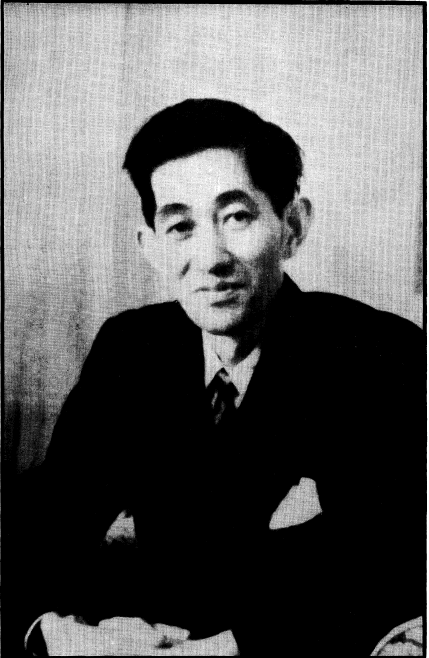
\includegraphics[height=180pt]{Nakayama.png} \\ \vspace{1em}
	\begin{minipage}{0.7\textwidth}
		\small Nakayama's Lemma is named after Tadashi Nakayama (1912---1964). Picture borrowed from \cite{obi-NAK}.
	\end{minipage}
\end{figure}

\begin{corollary}\label{prop:NAK-generation}
	Let $M$ be a finitely generated $R$-module, and let $I \subset \mathrm{rad}(R)$ be an ideal of $R$. If the images of $x_1, \ldots, x_n \in M$ in $M/IM$ form a set of generators, then $x_1, \ldots, x_n$ generate $M$.
\end{corollary}
\begin{proof}
	Apply Theorem \ref{prop:NAK} to $N := M/(Rx_1 + \cdots + Rx_n)$; our assumption $M = IM + Rx_1 + \cdots + Rx_n$ entails that $IN=N$, thus $N=0$.
\end{proof}

We record another amusing consequence of Theorem \ref{prop:NAK}.
\begin{proposition}
	Let $M$ be a finitely generated $R$-module and $\psi \in \End_R(M)$. If $\psi$ is surjective then $\psi$ is an automorphism.
\end{proposition}
\begin{proof}
	Introduce a variable $Y$. Make $M$ into an $R[Y]$-module by letting $Y$ act as $\psi$. Put $I := (Y)$ so that $IM=M$. Theorem \ref{prop:NAK} yields some $Q(Y) \in R[Y]$ satisfying $(1 - Q(Y)Y) M = 0$, that is, $Q(\psi)\psi = \identity_M$.
\end{proof}

\section{Noetherian and Artinian rings}
An $R$-module $M$ is called \emph{Noetherian} (resp. \emph{Artinian}) if every ascending (resp. descending) chain of submodules eventually stabilizes. Recall that in a short exact sequence $0 \to M' \to M \to M'' \to 0$, we have $M$ is Noetherian (resp. Artinian) if and only if $M'$ and $M''$ are. Being both Noetherian and Artinian is equivalent to being a module of \emph{finite length}\index{length}, that is, a module admitting composition series. \index{Artinian}\index{Noetherian}

If we take $M := R$ on which $R$ acts by multiplication, then the submodules are precisely the ideals of $R$. We say that $R$ is a Noetherian (resp. Artinian) ring if $R$ as an $R$-module is Noetherian (resp. Artinian); this translates into the corresponding chain conditions on the ideals. Both chain conditions are preserved under passing to quotients and localizations. Finitely generated modules over a Noetherian ring are Noetherian. The following result ought to be known to the readers.
\begin{theorem}[Hilbert's Basis Theorem] \index{Hilbert's basis theorem}
	If $R$ is Noetherian, then so is the polynomial algebra $R[X_1, \ldots, X_n]$ for any $n \in \Z_{\geq 1}$.
\end{theorem}
Joint with the foregoing remarks, we infer that finitely generated algebras over Noetherian rings are still Noetherian.

On the other hand, being Artinian is a rather stringent condition on rings.
\begin{theorem}\label{prop:Artinian-length}
	A ring $R$ is Artinian if and only if $R$ is of finite length as an $R$-module. Such rings are semi-local.
\end{theorem}
\begin{proof}
	As noticed before, having finite length implies that $R$ is Noetherian as well as Artinian. Assume conversely that $R$ is an Artinian ring. First we claim that $\MaxSpec(R)$ is finite, i.e. $R$ is semi-local. If there were an infinite sequence of distinct maximal ideals $\mathfrak{m}_1, \mathfrak{m}_2, \ldots$, we would have an infinite chain
	\[ \mathfrak{m}_1 \supset \mathfrak{m}_1 \mathfrak{m}_2 \supset \mathfrak{m}_1 \mathfrak{m}_2 \mathfrak{m}_3 \supset \cdots. \]
	This chain is strictly descending, since $\mathfrak{m}_1 \cdots \mathfrak{m}_i = \mathfrak{m}_1 \cdots \mathfrak{m}_{i+1}$ would imply $\mathfrak{m}_{i+1} \supset \mathfrak{m}_1 \cdots \mathfrak{m}_i$, hence $\mathfrak{m}_{i+1} \supset \mathfrak{m}_j$ for some $1 \leq j \leq i$ because maximal ideals are prime. From the Artinian property we conclude that there are only finitely many maximal ideals $\mathfrak{m}_1, \ldots, \mathfrak{m}_n$ of $R$.
	
	Set $\mathfrak{a} := \mathfrak{m}_1 \cdots \mathfrak{m}_n$. Since $R$ is Artinian we must have $\mathfrak{a}^k = \mathfrak{a}^{k+1}$ for some $k > 0$. We claim that $\mathfrak{a}^k = 0$.
	
	Put $\mathfrak{b} := \{r \in R: r\mathfrak{a}^k = 0 \}$, we have to show $\mathfrak{b}=R$. If not, let $\mathfrak{b}'$ be a minimal ideal lying strictly over $\mathfrak{b}$. Thus $\mathfrak{b}' = Rx + \mathfrak{b}$ for any $x \in \mathfrak{b}' \smallsetminus \mathfrak{b}$. We must have $\mathfrak{a}x + \mathfrak{b} \subsetneq \mathfrak{b}'$, for otherwise $M := \mathfrak{b}'/\mathfrak{b}$ is finitely generated (say by $x$) and satisfies $M = \mathfrak{a}M$, then Theorem \ref{prop:NAK} plus $\mathfrak{a} \subset \text{rad}(R)$ would imply $M = \{0\}$, which is absurd. By minimality we have $\mathfrak{b} = \mathfrak{a}x + \mathfrak{b}$. It follows that $\mathfrak{a}x \subset \mathfrak{b}$, i.e. $\mathfrak{a}^{k+1} x = 0$; from $\mathfrak{a}^k = \mathfrak{a}^{k+1}$ we infer $x \in \mathfrak{b}$. Contradiction.
	
	All in all, we obtain a descending chain of ideals
	\begin{align*}
		R & \supset \mathfrak{m}_1 \supset \mathfrak{m}_1 \mathfrak{m}_2 \supset \cdots \supset \mathfrak{m}_1 \cdots \mathfrak{m}_n = \mathfrak{a} \\
		& \supset \mathfrak{a} \mathfrak{m}_1 \supset \mathfrak{a} \mathfrak{m}_1 \mathfrak{m}_2 \supset \cdots \supset \mathfrak{a} \mathfrak{m}_1 \cdots \mathfrak{m}_n = \mathfrak{a}^2 \\
		& \supset \cdots \supset \mathfrak{a}^k = \{0\}.
	\end{align*}
	Each subquotient thereof, which is \textit{a priori} an $R$-module, is actually an $R/\mathfrak{m}_i$-vector space for some $1 \leq i \leq n$. Such a vector space must also satisfy the descending chain condition on vector subspaces, otherwise pulling-back will contradict the Artinian assumption on $R$. Artinian vector spaces must be finite-dimensional. It follows that all these subquotients are of finite length, hence so is $R$ itself.
\end{proof}

\begin{corollary}\label{prop:Artinian-dim-0}
	A ring $R$ is Artinian if and only if it is Noetherian and every prime ideal of $R$ is maximal.
\end{corollary}
\begin{proof}
	If $R$ is Artinian, then $R$ is of finite length, hence is Noetherian as well. For every prime ideal $\mathfrak{p}$, we have $\mathfrak{p} \supset \{0\} = (\mathfrak{m}_1 \cdots \mathfrak{m}_n)^k$ in the notations of the proof above, therefore $\mathfrak{p} \supset \mathfrak{m}_i$ for some $i$, so $\mathfrak{p} = \mathfrak{m}_i$ is maximal.

	Conversely, if $R$ is Noetherian but of infinite length, then the nonempty set of ideals
	\[ \mathcal{S} := \left\{ \text{ideals } I \subsetneq R: R/I \text{ has infinite length} \right\} \]
	contains a maximal element $\mathfrak{p}$. We contend that $\mathfrak{p}$ is prime. If $xy \in \mathfrak{p}$ with $x,y \notin \mathfrak{p}$, then $R/(\mathfrak{p}+Rx)$ has finite length by the choice of $\mathfrak{p}$; on the other hand, $\mathfrak{a} := \{ r \in R: rx \in \mathfrak{p}\} \supsetneq \mathfrak{p}$ (as $y \in \mathfrak{a}$), hence $R/\mathfrak{a}$ has finite length as well. From the short exact sequence $0 \to R/\mathfrak{a} \xrightarrow{x} R/\mathfrak{p} \to R/(\mathfrak{p}+Rx) \to 0$ we see $R/\mathfrak{p}$ has finite length, contradiction.
	
	If we assume moreover that every prime ideal is maximal, then for the $\mathfrak{p}$ chosen above, $R/\mathfrak{p}$ will be a field, thus of finite length. This is impossible.
\end{proof}

Rings whose prime ideals are all maximal are said to have \emph{dimension zero}, in the sense of Krull dimensions; we shall return to this point in \S\ref{sec:Krull-dimension}.

\section{What is commutative algebra?}
In broad terms, \emph{commutative algebra} is the study of commutative rings. Despite its intrinsic beauty, we prefer to motivate from an external point of view. See also \cite{Eis95}.

\begin{asparaenum}[(A)]
	\item \textbf{Algebraic geometry}\index{variety}. To simplify matters, we consider affine algebraic varieties over an algebraically closed field $\Bbbk$. Roughly speaking, such a variety is the zero locus $\mathcal{X} = \{ f_1 = \cdots = f_r = 0 \}$ in $\mathbb{A}^n = \Bbbk^n$ of $f_i \in \Bbbk[X_1, \ldots, X_n]$. The choice of equations is of course non-unique: what matters is the ideal $I(\mathcal{X}) := \{ f \in \Bbbk[X_1, \ldots, X_n] : f|_{\mathcal{X}} = 0 \}$. Conversely, every ideal $\mathfrak{a}$ defines a subset $V(\mathfrak{a}) := \{x \in \Bbbk^n : \forall f \in \mathfrak{a}, \; f(x)=0 \}$. As consequences of Hilbert's Nullstellensatz\index{Nullstellensatz}, which we will discuss later, we have
	\[ V \circ I(\mathcal{X}) = \mathcal{X}, \qquad I \circ V(\mathfrak{a})  = \sqrt{\mathfrak{a}}. \]
	One can deduce from this that the (closed) subvarieties of $\mathbb{A}^n$ are in bijection with ideals $\mathfrak{a}$ satisfying $\sqrt{\mathfrak{a}} = \mathfrak{a}$.

	Furthermore, $\Bbbk[\mathcal{X}] := \Bbbk[X_1, \ldots, X_n]/I(\mathcal{X})$ may be regarded as the ring of ``regular functions'' (i.e. functions definable by means of polynomials) on $\mathcal{X}$, and $\MaxSpec(\Bbbk[\mathcal{X}])$ is in bijection with the points of $\mathcal{X}$: to $x = (x_1, \ldots, x_n) \in \mathcal{X}$ we attach
	\[ \mathfrak{m}_x = (X_1 - x_1, \ldots, X_n - x_n) \supset I(\mathcal{X}). \]
	By passing to the ring $\Bbbk[\mathcal{X}]$, we somehow obtain a description of $\mathcal{X}$ that is independent of embeddings into affine spaces. Moreover, $\mathcal{X}$ inherits the Zariski topology from that on $\Spec(\Bbbk[\mathcal{X}])$.

	Naively speaking, the geometric properties of $\mathcal{X}$ transcribe in ring-theoretic terms to the reduced Noetherian $\Bbbk$-algebra $\Bbbk[\mathcal{X}]$. For example, assume that $f \in \Bbbk[\mathcal{X}]$ is not nilpotent, then the formation of $\Bbbk[\mathcal{X}][f^{-1}]$ corresponds to taking the Zariski-open subset $\mathcal{X}_f = \{x \in \mathcal{X}: f(x) \neq 0 \}$ of $\mathcal{X}$. This may be explained as follows:
	\[ \mathcal{X}_f \simeq \left\{ (x_1, \ldots, x_n, y) : f_1(x_1, \ldots, x_n) = \cdots = f_r(x_1, \ldots, x_n) = 0, \; f(x_1, \ldots, x_n)y = 1 \right\} \]
	which is also an affine algebraic variety in $\Bbbk^{n+1}$, and one may verify that $\Bbbk[\mathcal{X}_f] = \Bbbk[\mathcal{X}][f^{-1}]$.

	\item \textbf{Invariant theory}\index{invariant theory}. Let $G$ be a group acting on a finite-dimensional $\Bbbk$-vector space $V$ from the right, and let $\Bbbk[V]$ be the $\Bbbk$-algebra of polynomials on $V$. Thus $\Bbbk[V]$ carries a left $G$-action by $gf(v) = f(vg)$. For ``reasonable'' groups $G$, say finite or $\Bbbk$-algebraic ones, the classical invariant theory seeks to describe the subalgebra $\Bbbk[V]^G$ of invariants\footnote{More generally, we are also interested in the algebra of invariant differential operators with polynomial coefficients.} in terms of \emph{generators} and \emph{relations}.

	In particular, one has to know when is the algebra $\Bbbk[V]^G$ finitely generated. This is actually the source of many results in commutative algebra, such as the Basis Theorem and Nullstellensatz of Hilbert. For example, let the symmetric group $G = \mathfrak{S}_n$ act on $V = \Bbbk^n$ in the standard manner, then our question is completely answered by the following classical result: $\Bbbk[V]^G$ equals the polynomial algebra $\Bbbk[e_1, \ldots, e_n]$, where $e_i$ stands for the $i$-th elementary symmetric function in $n$ variables.

	The same questions may be posed for any affine algebraic variety $V$. From the geometric point of view, if $\Bbbk[V]^G$ is finitely generated, it will consist of regular functions of some kind of quotient variety $V /\!/ G$. The study of quotients in this sense naturally leads to \emph{geometric invariant theory}, for which we refer to \cite{AG4} for details.
\end{asparaenum}

	% To be compiled by XeLaTeX, preferably under TeX Live.
% LaTeX source for ``Yanqi Lake Lectures on Algebra'' Part III.
% Copyright 2019  李文威 (Wen-Wei Li).
% Permission is granted to copy, distribute and/or modify this
% document under the terms of the Creative Commons
% Attribution-NonCommercial 4.0 International (CC BY-NC 4.0)
% https://creativecommons.org/licenses/by-nc/4.0/

% To be included
\chapter{Primary decompositions}

We shall follow \cite[\S 3]{Eis95} and \cite[\S 8]{Mat80} closely.

\section{The support of a module}
Fix a ring $R$. For any $R$-module $M$ and $x \in M$, we define the \emph{annihilator} $\text{ann}_R(x) := \{ r \in R: rx=0 \}$; it is an ideal of $R$. Also define $\text{ann}_R(M) := \{r \in R: rM=0 \} = \bigcap_{x \in M} \text{ann}_R(x)$. \index{$\text{ann}_R(M), \text{ann}_R(x)$}

\begin{definition}\index{support}\index{SuppM@$\Supp(M)$}
	The \emph{support} of an $R$-module $M$ is
	\[ \Supp(M) := \left\{ \mathfrak{p} \in \Spec(R): M_{\mathfrak{p}} \neq 0 \right\}. \]
\end{definition}
Let us unwind the definition: $\mathfrak{p} \notin \Supp(M)$ means that every $x \in M$ maps to $0 \in M_{\mathfrak{p}}$, equivalently $\text{ann}_R(x) \not\subset \mathfrak{p}$. To test whether $\mathfrak{p} \notin \Supp(M)$, we only need to check the foregoing condition for $x$ ranging over a generating set of $M$.

\begin{proposition}
	If $M$ is finitely generated then $\Supp(M) = V(\mathrm{ann}_R(M))$; in particular it is Zariski-closed in $\Spec(R)$.
\end{proposition}
\begin{proof}
	Suppose $M = Rx_1 + \cdots + Rx_n$. Set $I_i := \text{ann}_R(x_i)$ and observe that $\bigcap_{i=1}^n I_i = \text{ann}_R(M)$. Then $\mathfrak{p} \in \Supp(M)$ if and only if $\mathfrak{p} \supset I_i$ for some $i$, that is, $\mathfrak{p} \in \bigcup_{i=1}^n V(I_i)$. To conclude, note that $V(I) \cup V(J) = V(IJ) = V(I \cap J)$ for any ideals $I, J \subset R$ (an easy exercise).
\end{proof}

Finite generation is needed in the result above. Consider the $\Z$-module $M := \bigoplus_{a \geq 1} \Z/p^a \Z$. Its support is $\{p\}$ but $\mathrm{ann}(M) = \{0\}$.

\begin{proposition}
	For an exact sequence $0 \to M' \to M \to M'' \to 0$ we have $\Supp(M) = \Supp(M') \cup \Supp(M'')$. For arbitrary direct sums we have $\Supp(\bigoplus_i M_i) = \bigcup_i \Supp(M_i)$.
\end{proposition}
\begin{proof}
	Again, we use the exactness of localization for the first assertion. For $\mathfrak{p} \in \Spec(R)$ we have an exact $0 \to M'_{\mathfrak{p}} \to M_{\mathfrak{p}} \to M''_{\mathfrak{p}} \to 0$, hence $M_{\mathfrak{p}} \neq 0$ if and only if $\mathfrak{p} \in \Supp(M') \cup \Supp(M'')$. The second assertion is obvious.
\end{proof}

From an $R$-module $M$, one can build a ``field of modules'' over $\Spec(R)$ by assigning to each $\mathfrak{p}$ the $R_{\mathfrak{p}}$-module $M_{\mathfrak{p}}$, and $\Supp(M)$ is precisely the subset of $M_{\mathfrak{p}}$ over which the field is non-vanishing. This is how the support arises in algebraic geometry. A more precise description will require the notion of quasi-coherent sheaves on schemes.

\begin{exercise}
	Let $M$, $N$ be finitely generated $R$-modules. Show that $\Supp(M \dotimes{R} N) = \Supp(M) \cap \Supp(N)$. Hint: since localization commutes with $\otimes$, it suffices to prove that $M \dotimes{R} N \neq \{0\}$ when $M, N$ are both nonzero finitely generated modules over a local ring $R$. Nakayama's Lemma implies that $M \dotimes{R} \Bbbk$ and $\Bbbk \dotimes{R} N$ are both nonzero where $\Bbbk$ is the residue field of $R$. Now
	\[ (M \dotimes{R} \Bbbk) \dotimes{\Bbbk} (\Bbbk \dotimes{R} N) \simeq M \dotimes{R} (\Bbbk \dotimes{\Bbbk} \Bbbk) \dotimes{R} N \simeq (M \dotimes{R} N) \dotimes{R} \Bbbk \]
	is nonzero.
\end{exercise}

\section{Associated primes}
Throughout this section, $R$ will be a Noetherian ring.

\begin{definition}\index{associated prime}\index{$\text{Ass}(M)$}
	A prime ideal $\mathfrak{p}$ is said to be an \emph{associated prime} of an $R$-module $M$ if $\text{ann}_R(x) = \mathfrak{p}$ for some $x \in M$; equivalently, $R/\mathfrak{p}$ embeds into $M$. Denote the set of associated primes of $M$ by $\text{Ass}(M)$.
\end{definition}

\begin{example}
	For the $\Z$-module $M := \Z/n\Z$ with $n \in \Z_{> 1}$, one easily checks that $\text{Ass}(M)$ is the set of prime factors of $n$.
\end{example}

\begin{lemma}\label{prop:Ass-maximal}
	Consider the set $\mathcal{S} := \{ \mathrm{ann}_R(x) : x \in M, \; x \neq 0 \}$ of ideals, partially ordered by inclusion. Every maximal element in $\mathcal{S}$ is prime.
\end{lemma}
\begin{proof}
	Let $\mathfrak{p} = \text{ann}_R(x)$ be a maximal element of $\mathcal{S}$ and suppose $ab \in \mathfrak{p}$. If $b \notin \mathfrak{p}$, then
	\[ bx \neq 0, \quad abx = 0, \quad R \neq \text{ann}_R(bx) \supset \text{ann}_R(x) = \mathfrak{p}. \]
	Hence $a \in \text{ann}_R(bx) = \mathfrak{p}$ by the maximality of $\mathfrak{p}$ in $\mathcal{S}$.
\end{proof}

\begin{definition}\index{zero divisor}
	Call $r \in R$ a \emph{zero divisor} on $M$ if $rx=0$ for some $x \in M \smallsetminus \{0\}$.
\end{definition}

\begin{theorem}\label{prop:Ass-properties}
	Let $M$ be an $R$-module.
	\begin{enumerate}[(i)]
		\item We have $M = \{0\}$ if and only if $\mathrm{Ass}(M) = \emptyset$.
		\item The union of all $\mathfrak{p} \in \mathrm{Ass}(M)$ equals the set of zero divisors on $M$.
		\item For any multiplicative subset $S \subset R$, we have
			\[ \mathrm{Ass}(M[S^{-1}]) = \left\{ \mathfrak{p}[S^{-1}] : \mathfrak{p} \in \mathrm{Ass}(M), \; \mathfrak{p} \cap S = \emptyset \right\} . \]
		\item If $0 \to M' \to M \to M''$ is exact, then $\mathrm{Ass}(M') \subset \mathrm{Ass}(M) \subset \mathrm{Ass}(M') \cup \mathrm{Ass}(M'')$.
	\end{enumerate}
\end{theorem}
\begin{proof}
	\begin{asparaenum}[(i)]
	\item Clearly $\text{Ass}(\{0\}) = \emptyset$. If $M \neq 0$, the set $\mathcal{S}$ in Lemma \ref{prop:Ass-maximal} is then nonempty, hence contains a maximal element $\mathfrak{p}$ because $R$ is Noetherian; this yields $\mathfrak{p} \in \text{Ass}(M)$.
	
	\item Elements of any $\mathfrak{p} \in \text{Ass}(M)$ are all zero divisors by the very definition of associated primes. Conversely, if $r \in \text{ann}_R(x)$ for some $x \in M \smallsetminus \{0\}$, there must exist some maximal element $\mathfrak{p}$ of $\mathcal{S}$ with $\mathfrak{p} \supset \text{ann}_R(x)$ as $R$ is Noetherian; so $\mathfrak{p}$ is the required associated prime containing $r$.
	
	\item If $\mathfrak{p} \in \Spec(R)$, $\mathfrak{p} \cap S = \emptyset$ and there is some $R/\mathfrak{p} \hookrightarrow M$, then
	\[ \{0\} \neq R[S^{-1}]/\mathfrak{p}[S^{-1}] \simeq (R/\mathfrak{p})[S^{-1}] \hookrightarrow M[S^{-1}] \]
	by the exactness of localizations, hence $\mathfrak{p}[S^{-1}] \in \text{Ass}(M[S^{-1}])$. Conversely, every element of $\text{Ass}(M[S^{-1}])$ has the form $\mathfrak{p}[S^{-1}]$ for some $\mathfrak{p} \in \Spec(R)$ disjoint from $S$. Also recall that $\mathfrak{p}$ equals the preimage of $\mathfrak{p}[S^{-1}]$ under $R \to R[S^{-1}]$. There exist $x \in M$ and $s \in S$ such that $\mathfrak{p}[S^{-1}] = \text{ann}_{R[S^{-1}]}(x/s) = \text{ann}_{R[S^{-1}]}(x)$. Ideals in a Noetherian ring being finitely generated, we infer that $\exists t \in S$ with $\mathfrak{p} \subset \text{ann}_R(tx)$. It remains to show $\mathfrak{p} = \text{ann}_R(tx)$. If $rtx=0$ for some $r \in R$, then $r$ maps into $r/1 \in \mathfrak{p}[S^{-1}] = \text{ann}_{R[S^{-1}]}(x)$; thus $r \in \mathfrak{p}$.

	\item It suffices to treat the second $\subset$. Suppose that $\mathfrak{p} \in \text{Ass}(M)$ and $R/\mathfrak{p} \simeq N$ for some submodule $N \subset M$. Identify $M'$ with $\Ker(M \to M'')$. If $M' \cap N = \{0\}$ then $R/\mathfrak{p} \simeq N \hookrightarrow M''$, so $\mathfrak{p} \in \text{Ass}(M'')$. If there exists $x \in M' \cap N \subset N$ with $x \neq 0$, then we have $\text{ann}_R(x) = \mathfrak{p}$ since $N \simeq R/\mathfrak{p}$ and $\mathfrak{p}$ is prime; in this case $\mathfrak{p} \in \text{Ass}(M')$.
	\end{asparaenum}
\end{proof}

We remark that $0 \to M' \to M \to M'' \to 0$ being exact does not imply $\text{Ass}(M) = \text{Ass}(M') \cup \text{Ass}(M'')$. To see this, consider $R=\Z$ and $0 \to \Z \xrightarrow{p} \Z \to \Z/p\Z \to 0$ for some prime number $p$.

\begin{exercise}
	Show that $\text{Ass}(M_1 \oplus M_2) = \text{Ass}(M_1) \cup \text{Ass}(M_2)$.
\end{exercise}

\begin{theorem}\label{prop:Supp-Ass}
	For every $R$-module $M$ we have $\Supp(M) = \bigcup_{\mathfrak{p} \in \mathrm{Ass}(M)} V(\mathfrak{p})$, in particular $\mathrm{Ass}(M) \subset \Supp(M)$.	Furthermore, every minimal element of $\Supp(M)$ with respect to inclusion is actually a minimal element of $\mathrm{Ass}(M)$.
\end{theorem}
\begin{proof}
	For any prime $\mathfrak{q}$ we have $M_{\mathfrak{q}} \neq 0 \iff \text{Ass}(M_{\mathfrak{q}}) \neq \emptyset$, and the latter condition holds precisely when there exists $\mathfrak{p} \in \text{Ass}(M)$ with $\mathfrak{p} \cap (R \smallsetminus \mathfrak{q}) = \emptyset$, i.e. $\mathfrak{q} \supset \mathfrak{p}$. This proves the first assertion. The second assertion is a direct consequence.
\end{proof}

Observe that if $\mathfrak{p} \in \Supp(M)$, then $\mathfrak{q} \supset \mathfrak{p} \implies \mathfrak{q} \in \Supp(M)$: the reason is that
\begin{gather}\label{eqn:localization-in-stages}
	M_{\mathfrak{p}} = (M_{\mathfrak{q}})_{\mathfrak{p}R_{\mathfrak{q}}}
\end{gather}
thus the occurrence of non-minimal elements in $\Supp(M)$ is unsurprising. In contrast, the non-minimal elements in $\text{Ass}(M)$ are somehow mysterious. These non-minimal associated primes are called \emph{embedded primes}. \index{embedded prime}

\begin{exercise}
	Prove the formula \eqref{eqn:localization-in-stages} of ``localization in stages''.
\end{exercise}

Hereafter we impose finite generation on $M$. This implies $M$ is Noetherian.
\begin{theorem}
	Let $M$ be a finitely generated $R$-module. There exists a chain $M = M_n \supset M_{n-1} \supset \cdots \supset M_0 = \{0\}$ of submodules such that for every $0 < i \leq n$, the subquotient $M_i/M_{i-1}$ is isomorphic to $R/\mathfrak{p}_i$ for some prime ideal $\mathfrak{p}_i$.
	
	Furthermore we have $\mathrm{Ass}(M) \subset \{\mathfrak{p}_1, \ldots, \mathfrak{p}_n \}$; in particular $\mathrm{Ass}(M)$ is a finite set.
\end{theorem}
\begin{proof}
	Assume $M \supsetneq M_0 := \{0\}$. There exists $\mathfrak{p}_1 \in \text{Ass}(M)$ together with a submodule $M_1 \subset M$ isomorphic to $R/\mathfrak{p}_1$. Furthermore $\text{Ass}(M_1) = \text{Ass}(R/\mathfrak{p}_1) = \{ \mathfrak{p}_1\}$ as easily seen. Hence the Theorem \ref{prop:Ass-properties} entails $\text{Ass}(M) \subset \{\mathfrak{p}_1\} \cup \text{Ass}(M/M_1)$.

	If $M_1 = M$ we are done. Otherwise we start over with $M/M_1$, finding $M_1 \subset M_2 \subset M$ with $M_2/M_1 \simeq R/\mathfrak{p}_2$ where $\mathfrak{p}_2 \in \text{Ass}_R(M/M_1)$, and so forth. This procedure terminates in finite steps since $M$ is Noetherian.
\end{proof}

\section{Primary and coprimary modules}
The classical framework of primary decompositions concerns ideals, but it is advantageous to allow modules here. As before, the ring $R$ is Noetherian.

\begin{definition}\index{coprimary module}\index{primary module}
	An $R$-module $M$ is called \emph{coprimary} if $\text{Ass}(M)$ is a singleton. A submodule $N \subsetneq M$ is called a $\mathfrak{p}$-\emph{primary} submodule if $M/N$ is coprimary with associated prime $\mathfrak{p} \in \Spec(R)$.
\end{definition}

\begin{proposition}\label{prop:coprimary-locnil}
	The following are equivalent for a nonzero $R$-module $M$.
	\begin{enumerate}[(i)]
		\item $M$ is coprimary;
		\item for every zero divisor $r \in R$ for $M$ and every $x \in M$, there exists $n \geq 1$ such that $r^n x = 0$.
	\end{enumerate}
\end{proposition}
The condition (ii) is usually called the local-nilpotency of $r$ on $M$. When $M = R/I$ for some ideal $I$, it translates into: all zero divisors of the ring $R/I$ are nilpotent.
\begin{proof}
	(i) $\implies$ (ii): Suppose $\text{Ass}(M) = \{ \mathfrak{p}\}$ and $x \in M \smallsetminus \{0\}$. From $\emptyset \neq \text{Ass}(Rx) \subset \text{Ass}(M)$ we infer that $\text{Ass}(Rx) = \{\mathfrak{p}\}$, thus by Theorem \ref{prop:Supp-Ass} we see $V(\mathfrak{p}) = \Supp(Rx) = V(\text{ann}(Rx))$. Hence $\mathfrak{p} = \sqrt{\text{ann}(Rx)}$. This implies (ii) by the definition of $\sqrt{\hspace{5pt}}$.
	
	(ii) $\implies$ (i): It is routine to check that
	\[ \mathfrak{p} := \left\{ r \in R: \forall x \in M \; \exists n \geq 1, \; r^n x = 0 \right\} \]
	is an ideal of $R$. For every $\mathfrak{q} \in \text{Ass}(M)$ there exists $x \in M$ with $\text{ann}_R(x) = \mathfrak{q}$. Every $r \in \mathfrak{p}$ has some power falling in $\mathfrak{q}$, thus $\mathfrak{p} \subset \mathfrak{q}$. Conversely, (ii) and Theorem \ref{prop:Ass-properties} imply $\mathfrak{q} = \text{ann}_R(x) \subset \mathfrak{p}$. From $\mathfrak{q}=\mathfrak{p}$ we conclude $M$ is coprimary with the unique associated prime $\mathfrak{p}$.
\end{proof}

\begin{exercise}[Classical definition of primary ideals]\label{ex:primary-ideal}
	Let $I$ be a proper ideal of $R$. Show that $R/I$ is coprimary if and only if the following holds:
	\[ \forall a,b \in R, \; (ab \in I) \wedge (a \notin I) \implies \exists n \geq 1, \; b^n \in I. \]
	In this case we also say $I$ is a \emph{primary ideal} of $R$. Show that $\{\sqrt{I}\} = \text{Ass}(R/I)$ if $I$ is a primary ideal. Hint: apply Proposition \ref{prop:coprimary-locnil}.
\end{exercise}

\begin{exercise}\label{ex:maximal-primary}
	Let $\mathfrak{m}$ be a maximal ideal of $R$. Show that every ideal $I \subsetneq R$ containing some power of $\mathfrak{m}$ is primary, and $\text{Ass}(R/I) = \{\mathfrak{m}\}$. Hint: show that $\mathfrak{m}$ is the only prime ideal containing $I = \text{ann}_R(R/I)$.
\end{exercise}

\begin{lemma}\label{prop:intersection-primary}
	Let $\mathfrak{p} \in \Spec(R)$ and $N_1, N_2 \subset M$ are $\mathfrak{p}$-primary submodules. Then $N_1 \cap N_2$ is a $\mathfrak{p}$-primary submodule of $M$.
\end{lemma}
\begin{proof}
	We have $M/N_1 \cap N_2 \hookrightarrow M/N_1 \oplus M/N_2$. Since $N_1 \cap N_2 \neq M$, we have
	\[ \emptyset \neq \text{Ass}(M/N_1 \cap N_2) \subset \text{Ass}(M/N_1) \cup \text{Ass}(M/N_2) = \{\mathfrak{p}\} \]
	by Theorem \ref{prop:Ass-properties}.
\end{proof}

\section{Primary decomposition: the main theorem}
We still assume $R$ Noetherian and fix a finitely generated $R$-module $M$.

\begin{theorem}[Lasker--Noether]\label{prop:primary-decomp}\index{primary decomposition}
	Let $N \subsetneq M$ be an $R$-submodule. Then we can express $N$ as
	\[ N = M_1 \cap \cdots \cap M_n, \]
	for some $n \geq 1$ and primary $R$-submodules $M_i$, say with $\mathrm{Ass}(M/M_i) = \{\mathfrak{p}_i\}$ for $i = 1, \ldots, n$. Such a decomposition is called a \emph{primary decomposition} of $N$. We say it is \emph{irredundant} if none of the $M_i$ can be dropped, and \emph{minimal} if there is no such decomposition with fewer terms.
	\begin{enumerate}[(i)]
		\item We have $\mathrm{Ass}(M/N) \subset \{ \mathfrak{p}_1, \ldots, \mathfrak{p}_n \}$, equality holds when the decomposition is irredundant.
		\item If the decomposition is minimal, then for every $\mathfrak{p} \in \mathrm{Ass}(M/N)$ there exists a unique $1 \leq i \leq n$ with $\mathfrak{p} = \mathfrak{p}_i$; consequently $n = |\mathrm{Ass}(M/N)|$.
		\item Consider a primary decomposition of $N$. Let $S \subset R$ be any multiplicative subset, and assume without loss of generality that $\mathfrak{p}_1, \ldots, \mathfrak{p}_m$ are the primes among $\{\mathfrak{p}_1, \ldots, \mathfrak{p}_n \}$ which are disjoint from $S$, then $m \geq 1 \iff N[S^{-1}] \subsetneq M[S^{-1}]$ and
		\[ N[S^{-1}] = M_1[S^{-1}] \cap \cdots \cap M_m[S^{-1}] \]
		is a primary decomposition of the $R[S^{-1}]$-submodule $N[S^{-1}] \subsetneq M[S^{-1}]$; this decomposition of $N[S^{-1}]$ is minimal if the one for $N$ is.
	\end{enumerate}
\end{theorem}
Note that the ``irredundant'' condition in \cite[(8.D)]{Mat80} corresponds to minimality here. The rings whose ideals all have primary decompositions are called \emph{Laskerian rings}, thus part (i) of the Theorem says Noetherian implies Laskerian, but there exist non-Noetherian examples.

\begin{proof}
	Establish the existence of primary decompositions first. Replacing $M$ by $M/N$, we may assume $N = \{0\}$ from the outset. We claim that
	\begin{gather}\label{eqn:Lasker-Noether-aux}
		\forall \mathfrak{p} \in \text{Ass}(M), \; \exists Q(\mathfrak{p}) \subset M, \;
		\left\{ \begin{array}{l}
			Q(\mathfrak{p}) \text{ is } \mathfrak{p}\text{-primary}, \\
			\text{Ass}(Q(\mathfrak{p})) = \text{Ass}(M) \smallsetminus \{ \mathfrak{p} \}. 
		\end{array}\right.
	\end{gather}
	Granting this, $Q := \bigcap_{\mathfrak{p} \in \text{Ass}(M)} Q(\mathfrak{p})$ yields the required decomposition since $\text{Ass}(M)$ is finite and $\text{Ass}(Q) = \emptyset$.
	
	Establish \eqref{eqn:Lasker-Noether-aux} as follows. Put $\Psi := \{ \mathfrak{p} \}$. By Zorn's Lemma\index{Zorn's Lemma} we get a maximal element $Q(\mathfrak{q})$ from the set
	\[ \emptyset \neq \left\{  Q \subset M: \text{submodule}, \; \text{Ass}(Q) \subset \text{Ass}(M) \smallsetminus \Psi \right\} \]
	which is partially ordered by inclusion (details omitted, and you may also use the Noetherian property of $M$). Since
	\[ \text{Ass}(M) \subset \text{Ass}(M/Q(\mathfrak{p})) \cup \text{Ass}(Q(\mathfrak{p})), \]
	it suffices to show $\text{Ass}(M/Q(\mathfrak{p})) \subset \Psi$.  Let $\mathfrak{q} \in \text{Ass}(M/Q(\mathfrak{p}))$ so that there exists $M \supset Q' \supset Q(\mathfrak{p})$ with $Q'/Q(\mathfrak{p}) \simeq R/\mathfrak{q}$. Since $\text{Ass}(Q') \subset \text{Ass}(Q(\mathfrak{p})) \cup \{ \mathfrak{q} \}$, maximality forces $\mathfrak{q} \in \Psi$ (otherwise $\text{Ass}(Q') \subset \text{Ass}(M) \smallsetminus \Psi$), whence \eqref{eqn:Lasker-Noether-aux}. Now we turn to the properties (i) --- (iii).
	
	\begin{asparaenum}[(i)]
		\item The obvious embedding
		\[ M/N \hookrightarrow \bigoplus_{i=1}^n M/M_i \]
		together with Theorem \ref{prop:Ass-properties} yield $\text{Ass}(M/N) \subset \bigcup_{i=1}^n \text{Ass}(M/M_i) = \{ \mathfrak{p}_1, \ldots, \mathfrak{p}_n \}$.
		
		Now assume the given primary decomposition is irredundant, we have
			\begin{align*}
				\{0\} & \neq \frac{M_2 \cap \cdots \cap M_n}{N} = \frac{M_2 \cap \cdots \cap M_n}{M_1 \cap (M_2 \cap \cdots \cap M_n)} \\
				& \simeq \frac{M_1 + M_2 \cap \cdots \cap M_n}{M_1} \hookrightarrow M/M_1.
			\end{align*}
			Thus $\text{Ass}(M/N)$ contains $\text{Ass}((M_2 \cap \cdots \cap M_n)/N) = \{\mathfrak{p}_1\}$. Same for $\mathfrak{p}_2, \ldots, \mathfrak{p}_n$.
		\item Suppose $N = M_1 \cap \cdots \cap M_n$ is an irredundant primary decomposition, so that $\text{Ass}(M/N) = \{ \mathfrak{p}_1, \ldots, \mathfrak{p}_n \}$. If $\mathfrak{p}_i = \mathfrak{p}_j$ for some $1 \leq i \neq j \leq n$, Lemma \ref{prop:intersection-primary} will imply that $M_i \cap M_j$ is primary, leading to a shorter primary decomposition. This is impossible when the primary decomposition is minimal.
		\item Suppose $S \cap \mathfrak{p}_i = \emptyset$ (equivalently, $i \leq m$). By Theorem \ref{prop:Ass-properties} and the exactness of localization, $M_i[S^{-1}] \subset M[S^{-1}]$ will be $\mathfrak{p}_i[S^{-1}]$-primary. On the other hand $S \cap \mathfrak{p}_i \neq \emptyset$ implies $\text{Ass}((M/M_i)[S^{-1}]) = \emptyset$ by Theorem \ref{prop:Ass-properties}, thus $M[S^{-1}]/M_i[S^{-1}] = 0$. Since localization respects intersections, we obtain
		\[ N[S^{-1}] = \bigcap_{i=1}^m M_i[S^{-1}]. \]
		In particular $N[S^{-1}]$ is proper if and only if $m \geq 1$.
	
		It remains to show $\text{Ass}(M[S^{-1}]/N[S^{-1}])$ has $m$ elements if the original primary decomposition is minimal. Indeed, that set is just $\{ \mathfrak{p}[S^{-1}] : \mathfrak{p} \in \text{Ass}(M/N), \; \mathfrak{p} \cap S = \emptyset \}$ by Theorem \ref{prop:Ass-properties}, which equals $\{ \mathfrak{p}_1[S^{-1}], \ldots, \mathfrak{p}_m[S^{-1}] \}$ (distinct) by (ii).
	\end{asparaenum}
\end{proof}

A natural question arises: to what extent are minimal primary decompositions unique? For those $M_i$ whose associated primes are minimal in $\text{Ass}(M/N)$, the answer turns out to be positive.

\begin{corollary}\label{prop:p-primary-component}
	Let $N = M_1 \cap \cdots \cap M_n$ be a minimal primary decomposition of $N \subsetneq M$. Suppose that $M_1$ is $\mathfrak{p}$-primary where $\mathfrak{p} := \mathfrak{p}_1$ is a minimal element in $\mathrm{Ass}(M/N)$, then $M_1$ equals the preimage of $N_{\mathfrak{p}}$ under $M \to M_{\mathfrak{p}}$. Call it the $\mathfrak{p}$-\emph{primary component} of $N$.
\end{corollary}
\begin{proof}
	Recall the proof of Theorem \ref{prop:primary-decomp}, especially the part (iii); here we localize with respect to $S := R \smallsetminus \mathfrak{p}$. The minimality assumption entails
	\[ N_{\mathfrak{p}} = M_{1, \mathfrak{p}} \subset M_{\mathfrak{p}}. \]
	It remains to show that the preimage of $M_{1, \mathfrak{p}}$ under $M \to M_{\mathfrak{p}}$ equals $M_1$, in other words the injectivity of the natural map $M/M_1 \to (M/M_1)_{\mathfrak{p}} = M_{\mathfrak{p}}/M_{1, \mathfrak{p}}$. Indeed, $\bar{x} \in M/M_1$ maps to $0$ if and only if there exists $s \notin \mathfrak{p}$ with $s\bar{x}=0$, but Theorem \ref{prop:Ass-properties} implies that the zero divisors of $M/M_1$ must lie in $\mathfrak{p}$.
\end{proof}

It follows that the non-uniqueness of minimal primary decompositions can only arise from embedded primes in $\text{Ass}(M/N)$.

\section{Examples and remarks}
Primary decompositions are most often applied in the case $M = R$ and $N = I$ is a proper ideal. The goal is to express $I$ as an intersection of primary ideals. To begin with, let us take $R = \Z$. Observations:
\begin{itemize}
	\item The primary ideals of $R$ take the form $(p)^n$, where $n \geq 1$ and $p$ is a prime number or zero. This may be deduced from Exercise \ref{ex:primary-ideal} or directly from definitions.
	\item The irredundant primary decompositions of $\Z/n\Z$, for $n > 1$, corresponds to the factorization of $n$ into prime-powers. There are no embedded primes in this case; the irredundant primary decomposition is unique and automatically minimal.
\end{itemize}

\begin{exercise}
	Justify the foregoing assertions.
\end{exercise}

\begin{figure}[h]
	\centering 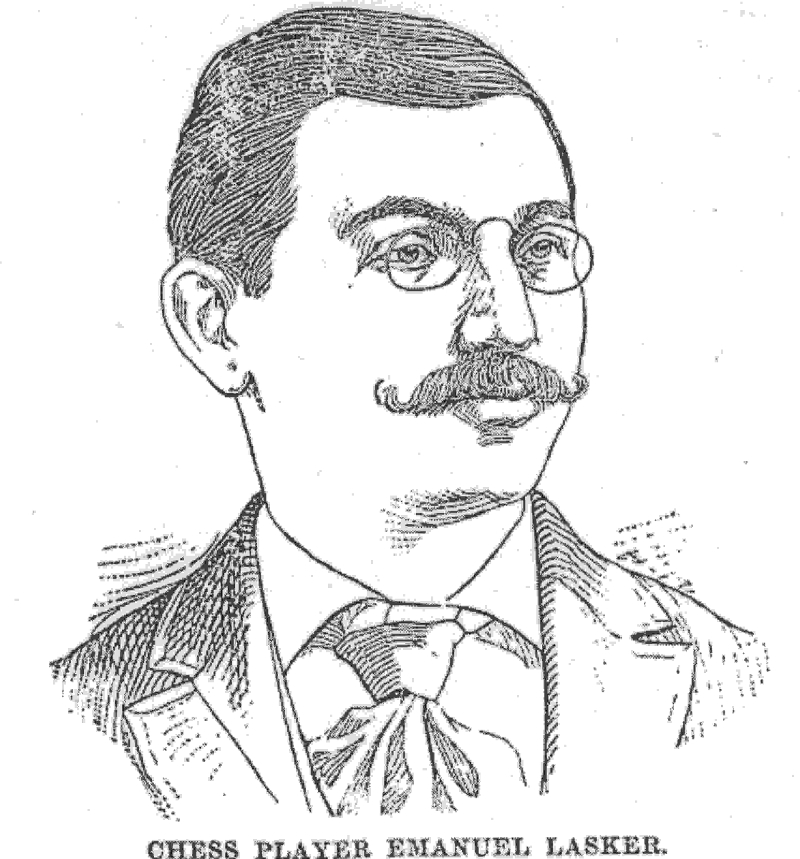
\includegraphics[height=170pt]{ELasker.jpg} \\ \vspace{1em}
	\begin{minipage}{0.7\textwidth}
		\small Emanuel Lasker (1868--1941) first obtained the primary decomposition for finitely generated $\Bbbk$-algebras and the algebras of convergent power series in 1905. His method involves techniques from \emph{elimination theory}. His result is then generalized and rewritten by Emmy Noether in 1921, in which the ascending chain condition plays a pivotal role. Lasker is best known for being the World Chess Champion from 1894 to 1921. (Picture taken from \href{https://commons.wikimedia.org/w/index.php?curid=5676713}{Wikimedia Commons})
	\end{minipage}
\end{figure}

Therefore one can regard primary decompositions as a generalization of factorization of integers, now performed on the level of ideals. The most important case is $R = \Bbbk[X_1, \ldots, X_n]$ (fix some field $\Bbbk$), as it is naturally connected to classical problems in algebraic geometry. Let us consider a simple yet non-trivial example from \cite[\S 3]{Eis95}.

\begin{example}
	Take $R=\Bbbk[X,Y]$ and $I = (X^2, XY)$. The reader is invited to check that
	\[ I = (X) \cap (X^2, XY, Y^2) = (X) \cap (X^2, Y). \]
	Claim: this gives two minimal primary decompositions of $I$. The ideal $(X)$ is prime, hence primary. In fact, $(X^2, XY, Y^2) = (X,Y)^2$ and $(X^2, Y)$ are both primary ideals associated to the maximal ideal $(X, Y)$. This follows either by direct arguments or by Exercise \ref{ex:maximal-primary}, noting that $(X,Y)^2 = (X^2, XY, Y^2)$ is contained in $(X^2, Y)$. The embedded prime $(X,Y)$ is seen to be responsible non-uniqueness of primary decompositions.
	
	To see the geometry behind, recall that $V(\mathfrak{a}) \cup V(\mathfrak{b}) = V(\mathfrak{a}\mathfrak{b}) = V(\mathfrak{a} \cap \mathfrak{b})$ for any ideals $\mathfrak{a}, \mathfrak{b}$, thus expressing $I$ as an intersection means breaking the corresponding geometric object into a union of simpler pieces. Also recall that for an ideal $I \subset \Bbbk[X,Y]$, the points in $\bigcap_{f \in I} \{f=0\}$ are in bijection with the maximal ideals lying over $I$, at least for $\Bbbk$ algebraically closed (Nullstellensatz). Thus we may interpret these primary decompositions as equalities among ``geometric objects'' embedded in $\Bbbk^2$:
	\[ \left\{ X^2=0, XY=0 \right\} = \begin{cases} \left\{ X = 0 \right\} \cup \left\{X^2=XY=Y^2=0 \right\} \\ \left\{ X = 0 \right\} \cup \left\{ X^2=Y=0 \right\}. \end{cases} \]
	\begin{enumerate}
		\item The geometric object defined by $X=0$ inside $\Bbbk^2$ is certainly the $Y$-axis: the regular functions living on this space form the $\Bbbk$-algebra $\Bbbk[X,Y]/(X) = \Bbbk[Y]$.
		\item The geometric object defined by $X^2=XY=Y^2=0$ looks ``physically'' like the origin $(0,0)$, but the $\Bbbk$-algebra of ``regular functions'' (in an extended sense) living on it equals $\Bbbk[X,Y]/(X^2,XY,Y^2)$: by restricting a polynomial function $f(X,Y)$ to this ``thickened point'', we see not only $f(0,0)$ but also $\frac{\partial f}{\partial x}(0,0)$ and $\frac{\partial f}{\partial y}(0,0)$. In other words, we shall view $X^2=XY=Y^2=0$ as the first-order infinitesimal neighborhood of $(0,0) \in \Bbbk^2$.
		\item In a similar vein, $X^2=Y=0$ physically defines $(0,0)$, but by restricting $f$ to that thickened point, we retrieve $f(0,0)$ as well as $\frac{\partial f}{\partial x}(0,0)$. Therefore we obtain the first-order infinitesimal neighborhood of $0$ inside the $X$-axis.
	\end{enumerate}

	Both decomposition says that we obtain the $Y$-axis together with first-order infinitesimal information at the origin $(0,0)$. This is also a nice illustration of the use of nilpotent elements in scheme theory.
\end{example}

\begin{example}[Symbolic powers]
	Let $\mathfrak{p}$ be a prime ideal in a Noetherian ring $R$ and fix $n \geq 1$. Observe that $\mathfrak{p}$ is the unique minimal element in $\Supp(R/\mathfrak{p}^n) = V(\mathfrak{p}^n)$. By Theorem \ref{prop:Supp-Ass} $\mathfrak{p} \in \text{Ass}(R/\mathfrak{p}^n)$, so it makes sense to denote by $\mathfrak{p}^{(n)}$ the $\mathfrak{p}$-primary component (Corollary \ref{prop:p-primary-component}) of $\mathfrak{p}^n$, called the $n$-th \emph{symbolic power} of $\mathfrak{p}$. In general $\mathfrak{p}^{(n)} \supsetneq \mathfrak{p}^n$. For a nice geometric interpretation of symbolic powers due to Nagata and Zariski, we refer to \cite[\S 3.9]{Eis95}.
\end{example}

Getting primary decomposition of ideals in polynomial algebras is a non-trivial task. Thanks to the pioneers in computational commutative algebra, this can now achieved on your own computer, eg. by the open-source \href{http://www.sagemath.org}{SageMath} system.\index{SageMath}
	% To be compiled by XeLaTeX, preferably under TeX Live.
% LaTeX source for ``Yanqi Lake Lectures on Algebra'' Part III.
% Copyright 2019  李文威 (Wen-Wei Li).
% Permission is granted to copy, distribute and/or modify this
% document under the terms of the Creative Commons
% Attribution-NonCommercial 4.0 International (CC BY-NC 4.0)
% https://creativecommons.org/licenses/by-nc/4.0/

% To be included
\chapter{Integral dependence, Nullstellensatz and flatness}

The materials below largely come from \cite[\S 4]{Eis95}, \cite[V.4]{AK70} and \cite[\S\S 5--6]{Mat80}. In what follows, any ring $R$ and the $R$-algebras are assumed to be commutative. For elements $a,b, \ldots$ in an $R$-algebra, denote by $R[a,b, \ldots]$ the $R$-subalgebra generated by them.

\section{Integral extensions}
Consider an $R$-algebra $A$. Recall that to give an $R$-algebra $A$ is the same as to give a ring homomorphism $\varphi: R \to A$. We shall switch freely between algebra and homomorphisms, omitting $\varphi$ if necessary. In many concrete circumstances $R$ is simply a subring of $A$.

\begin{definition}\index{integrality}
	An element $x \in A$ is said to be \emph{integral} over $R$ if there exists a monic polynomial $P(X) = X^n + a_{n-1} X^{n-1} + \cdots + a_0 \in R[X]$ (with $n \geq 1$) such that $P(x)=0$. If every $x \in A$ is integral over $R$, we say $A$ is integral over $R$.
\end{definition}
Note that elements from $R$ are trivially integral: take $P(X)$ with $n=1$. In the case $A = \CC$ and $R = \Z$, we recover the notion of \emph{algebraic integers}.

When $R$ is a field, we usually say \emph{algebraic} instead of \emph{integral}. The monic assumption on $P$ is crucial when $R$ is not a field, as illustrated by the following proof.

\begin{proposition}
	An element $x \in A$ is integral over $R$ if and only if there exists an $R$-submodule $M \subset A$ such that
	\begin{compactitem}
		\item $M$ is a finitely generated $R$-module;
		\item $xM \subset M$, thus $M$ is an $R[x]$-module;
		\item $M$ is a faithful $R[x]$-module i.e. $\mathrm{ann}_{R[x]}(M) = \{0\}$, and
	\end{compactitem}
	If $x$ is integral, $M := R[x]$ satisfies the conditions listed above.
\end{proposition}
\begin{proof}
	This is a familiar application of Cayley-Hamilton theorem, which we recall below. If $x$ is integral, say $x^n + a_{n-1} x^{n-1} + \cdots + a_0 = 0$, a straightforward induction shows that
	\[ R[x] = \sum_{i=0}^{n-1} Rx^i. \]
	In particular we may take $M := R[x]$ to be the required submodule, which is faithful as $1 \in R[x]$. Conversely, given a submodule $M$ as above, with generators $x_1, \ldots, x_m$, we make $M$ into an $R[X]$-module by letting the variable $X$ act as multiplication by $x$. Writing $x \cdot x_i = \sum_{j=1}^m a_{ij} x_j$, there is the matrix equation
	\[ (X \cdot 1_{m \times m} - A) \begin{pmatrix} x_1 \\ \vdots \\ x_m \end{pmatrix} = 0, \quad A = (a_{ij})_{1 \leq i,j \leq m} \in \text{Mat}_{m \times m}(R) \]
	over $R[X]$. Now multiply both sides by the cofactor matrix $(X \cdot 1_{m \times m} - A)^\vee$, we get $P(X) x_i = 0$ for all $i$, where $P \in R[X]$ is the characteristic polynomial of $A$, i.e. $P(x)M = \{0\}$. Since $M$ is faithful as an $R[x]$-module, we get $P(x)=0$.
\end{proof}

\begin{corollary}
	The integral elements in an $R$-subalgebra $A$ form a subalgebra. In particular, $A$ is integral over $R$ if and only if it has a set of integral generators.
\end{corollary}
\begin{proof}
	Let $a, b \in A$ be integral elements. One readily checks that
	\begin{itemize}
		\item $R[a,b]$ is finitely generated as an $R$-module (say by certain monomials $a^i b^j$);
		\item $R[a,b]$ is faithful (as an $R[a,b]$-module) because it contains $1$.
	\end{itemize}
	Thus $R[a,b]$ witnesses the integrality of $a+b$ and $ab$, since they both stabilize $R[a,b]$.
\end{proof}

\begin{proposition}\label{prop:integrality-tower}
	Consider ring homomorphisms $R \to A \to B$ such that $A$ is integral over $R$. If $y \in B$ is integral over $A$, then it is integral over $R$. 
\end{proposition}
\begin{proof}
	Assume $y^n + a_{n-1} y^{n-1} + \cdots + a_0 = 0$ with $a_0, \ldots, a_{n-1} \in A$ integral over $R$. The $R[a_0, \ldots, a_{n-1}]$-module $R[a_0, \ldots, a_{n-1}][y]$ is also finitely generated over $R$, faithful and preserved by $y$, hence it witnesses the integrality of $y$ over $R$.
\end{proof}

This subalgebra of integral elements in $A$ is called the \emph{integral closure}\index{integral closure} of $R$ in $A$. If the integral closure equals the image of $R$ in $A$, we say $R$ is \emph{integrally closed} in $A$. The integral closure is automatically integrally closed by virtue of Proposition \ref{prop:integrality-tower}.

\begin{definition}\index{normal}
	Let $R$ be an integral domain and denote by $K$ its field of fractions. The integral closure of $R$ in $K$ is called the \emph{normalization} of $R$. The domain $R$ is said to be \emph{normal} if $R$ is integrally closed in $K$.
\end{definition}

The first examples of normal domains come from unique factorization domains (UFD) that you have seen in undergraduate algebra, including $\Z$, $\Q[X,Y]$, etc.

\begin{proposition}
	Unique factorization domains are normal.
\end{proposition}
\begin{proof}
	Given $x = r/s \in K$ with coprime $r,s \in R$. If there is an integral dependence relation $x^n + a_{n-1} x^{n-1} + \cdots + a_0 = 0$, we will have $r^n + a_{n-1} r^{n-1}s + \cdots + a_0 s^n = 0$, hence $s \mid r^n$. As $r$ is coprime to $s$, we see $s \in R^\times$ and $x \in R$.
\end{proof}

Let us show that taking integral closure commutes with localizations. Geometrically, this means that taking integral closure is a local operation on $\Spec(R)$.

\begin{lemma}
	Let $A$ be an $R$-algebra, $S$ be a multiplicative subset of $R$. Denote by $\tilde{R}$ the integral closure of $R$ in $A$. Then the integral closure of $R[S^{-1}]$ in $A[S^{-1}]$ equals $\tilde{R}[S^{-1}]$.
\end{lemma}
\begin{proof}
	Suppose that $x \in A$ satisfies $x^n + \sum_{i=0}^{n-1} b_i x^i = 0$ with $b_0, \ldots, b_{n-1} \in R$. For all $s \in S$ we deduce $\left(\frac{x}{s}\right)^n + \sum_{i=0}^{n-1} \frac{b_i}{s^{n-i}} \cdot \left( \frac{x}{s} \right)^i = 0$ in $A[S^{-1}]$. Therefore $\tilde{R}[S^{-1}]$ is in the integral closure of $R[S^{-1}]$ in $A[S^{-1}]$.

	Conversely, suppose that $x/s \in A[S^{-1}]$ satisfies
	\[ \left(\frac{x}{s}\right)^n + \sum_{i=0}^{n-1} \frac{a_i}{s_i} \left( \frac{x}{s} \right)^i = 0, \quad a_i \in A, \; s_i \in S. \]
	Cleaning denominators, we see that $x s_1 \cdots s_{n-1}$ is integral over $R$, hence $x = \frac{xs_1 \cdots s_{n-1}}{s_1 \cdots s_n} \in \tilde{R}[S^{-1}]$.
\end{proof}

In particular, localizations of a normal domain are still normal. We have the following converse.
\begin{exercise}
	Let $R$ be a domain. If for every maximal ideal $\mathfrak{m}$ of $R$ we have $R_{\mathfrak{m}}$ is normal, then so is $R$ itself. Hint: recall that $R = \bigcap_{\mathfrak{m}} R_{\mathfrak{m}}$ inside the fraction field $K$.
\end{exercise}

\begin{exercise}
	Let $R := \CC[X,Y]/(Y^2-X^3)$. Show that
	\begin{compactenum}[(i)]
		\item $R$ is a domain, or equivalently, $Y^2 - X^3$ is an irreducible polynomial;
		\item the element $x := \bar{Y}/\bar{X} \in \text{Frac}(R)$ does not lie in $R$, where $\bar{X},\bar{Y}$ denote the images of $X,Y \in \CC[X,Y]$;
		\item show that $x^3 \in R$, therefore $R$ is not a normal ring.
	\end{compactenum}
\end{exercise}

\begin{remark}
	The rationale of the previous Exercise comes from singularity. Consider the \emph{cuspidal curve} $C := \{ (x,y) \in \CC^2: y^2=x^3\}$. It has an isolated singularity at $(0,0)$ since $\nabla (y^2-x^3) = (0,0)$ at the origin. On the other hand, it admits a (non-injective) parametrization from $\CC$ by
	\[ t \mapsto (x=t^2, y=t^3). \]
	Following Milnor \cite{Mil68}, a nice way to understand the ``cusp'' at $(0,0)$ is to cut $C$ by a $3$-sphere $S := \{(x,y) \in \CC^2: |x|^2 + |y|^2 = \epsilon \}$ enclosing the origin, with $0 < \epsilon \ll 1$. Writing the parametrization above as $t=re^{i\theta}$ in polar coordinates, we get the equation $r^4 + r^6 = \epsilon$ which has a unique positive root $\rho$. Hence $S \cap C$ is described by the closed curve $\theta \mapsto (\rho^2 e^{2i\theta}, \rho^3 e^{3i\theta})$ in $S \simeq \mathbb{S}^3$. We call $S \cap C$ the \emph{link of singularity} at $(0,0)$; in this case it is equivalent to the $(2,3)$-torus knot, i.e. the \emph{trefoil} shown below.
	
	\begin{center}\vspace{1.5em}
		% Draw the trefoil knot using the knots library in TikZ
		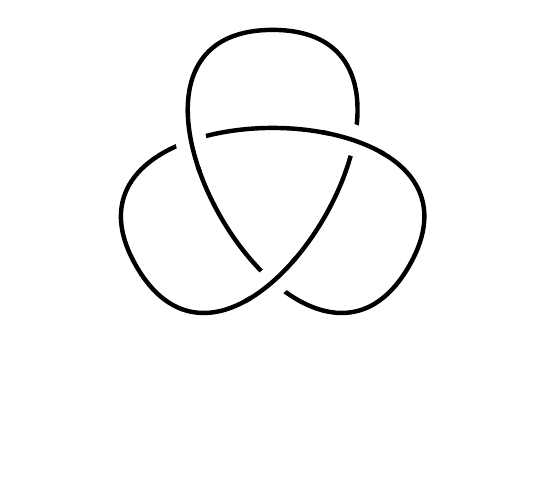
\begin{tikzpicture}
			\begin{knot}[
				consider self intersections,
				flip crossing = 2,
				clip width = 7]
			\strand[ultra thick, black]
				(90:2) to[out=180, in=-120, looseness=2]
				(-30:2) to[out=60, in=120, looseness=2]
				(210:2) to[out=-60, in=0, looseness=2] (90:2);
			\end{knot}
		\end{tikzpicture}
	\end{center}

	If we started from a non-singular curve in $\CC^2$, the result would then be an unknotted $\mathbb{S}^1$ inside $\mathbb{S}^3$. In this sense the link provides a measure for the singularity.
\end{remark}


Our study of normality has to be paused here. We refer to \cite[\S\S 8--9]{Mum99} for a beautiful discussion on the algebro-geometric content of normality, as well as important consequences such as Zariski's Main Theorem. Roughly speaking, normality means there is only one branch through each point of the corresponding variety.

\section{Nullstellensatz}
Our aim is to present a generalization of the celebrated \emph{Nullstellensatz}, which is one of the cornerstones of algebraic geometry. We shall also write the nilpotent radical of a ring $R$ as
\[ \text{nil}(R) := \sqrt{0_R}. \]
For an ideal $\mathfrak{a} \subset R$, we write $\mathfrak{a}[X]$ for the ideal of $R[X]$ formed by polynomials with all coefficients lying in $\mathfrak{a}$.

\begin{definition}\label{def:Jacobson-ring}\index{Jacobson ring}
	A ring $R$ is called a \emph{Jacobson ring} if every prime ideal $\mathfrak{p}$ satisfies
	\begin{gather}\label{eqn:Hilbert}
		\mathfrak{p} = \bigcap_{\mathfrak{m}: \text{maximal ideal } \supset \mathfrak{p}} \mathfrak{m}.
	\end{gather}
	Equivalently, we require that the Jacobson radical $\text{rad}(R/\mathfrak{p}) = \text{nil}(R/\mathfrak{p}) = \{0\}$ for all $\mathfrak{p}$. Note that $\supset$ always holds.
\end{definition}
Observations:
\begin{compactitem}
	\item Quotients of Jacobson rings are still Jacobson.
	\item Fields are trivially Jacobson.
\end{compactitem}

\begin{exercise}
	Prove that every principal ideal domain (a domain in which every ideal is generated by one element) with infinitely many maximal ideals is Jacobson.
\end{exercise}


\begin{theorem}[E.\ Snapper]\label{prop:Snapper}
	For any $R$, the polynomial algebra $R[X]$ satisfies $\mathrm{rad}(R[X]) = \mathrm{nil}(R[X])$.
\end{theorem}
\begin{proof}
	To show that $\text{nil}(R[X]) \supset \text{rad}(R[X])$, let $f(X) = \sum_i a_i X^i \in \text{rad}(R[X])$, then $1+Xf(X) = 1 + \sum_i a_i X^{i+1} \in R[X]^\times$. By looking at the reduction modulo $\mathfrak{p}$ of $f(X)$ for every prime ideal $\mathfrak{p}$ of $R$, we see that $a_i \in \bigcap \mathfrak{p} = \text{nil}(R)$ for all $i$. Hence $f(X) \in \text{nil}(R)[X] \subset \text{nil}(R[X])$.
\end{proof}

\begin{lemma}
	Let $R \subset A$ be integral domains such that $A$ is a finitely generated $R$-algebra. If $\mathrm{rad}(R)=\{0\}$, then $\mathrm{rad}(A)=\{0\}$.
\end{lemma}
\begin{proof}
	We may assume that $A$ is generated by a single element $a \in A$ over $R$. If $a$ is transcendental over $K := \text{Frac}(R)$, Theorem \ref{prop:Snapper} above can be applied as $\mathrm{nil}(R[X]) = \{0\}$. Let us assume that $a$ satisfies $f(a)=0$ for some $f(X) = \sum_{i=0}^n r_i X^i \in R[X]$ with $r_n \neq 0$. Let $b \in \text{rad}(A)$ and suppose $b \neq 0$. Hereafter we embed everything into the $K$-algebra $\text{Frac}(A)$. Since $a$ is algebraic over $K$, so is every element from $R[a]$ or even $K[a] \subset \text{Frac}(A)$. Hence $b$ is integral over $K$ as well. By cleaning denominators, we arrive at $g(b)=0$ for some $g(X) = \sum_{i=0}^m s_i X^i \in R[X]$ with the smallest possible degree $m$. Since $A$ is a domain, we have $s_0 \neq 0$.

	Using $\text{rad}(R) =\{0\}$, there exists a maximal ideal $\mathfrak{m}$ of $R$ such that $r_n s_0 \not\in \mathfrak{m}$. Taking localization at $\mathfrak{m}$, we get the subring $A' := A \otimes_R R_{\mathfrak{m}} \subset \text{Frac}(A)$ containing $R_{\mathfrak{m}}$, and $A'$ is also a finitely generated $R_{\mathfrak{m}}$-module since we inverted $r_n$. Nakayama's Lemma for $R_{\mathfrak{m}}$-modules implies $\mathfrak{m} A' \subsetneq A'$, thus $\mathfrak{m} A \subsetneq A$. Now choose a maximal ideal $\mathfrak{m}_A$ of $A$ over $\mathfrak{m}$. We must have $\mathfrak{m}_A \cap R = \mathfrak{m}$, which entails $s_0 \not\in \mathfrak{m}_A$. This is a contradiction since $s_0 = -\sum_{i=1}^m s_i b^i \in \text{rad}(A)$.
\end{proof}

\begin{theorem}[Nullstellensatz]\label{prop:Nullstellensatz-gen}\index{Nullstellensatz}
	Let $A$ be a finitely generated $R$-algebra. Assume that $R$ is a Jacobson ring, then the following statements hold.
	\begin{enumerate}[(i)]
		\item $A$ is a Jacobson ring.
		\item Let $\mathfrak{n} \in \Spec(A)$ be maximal, then its image $\mathfrak{m} \in \Spec(R)$ is maximal as well, and $A/\mathfrak{n}$ is a finite extension of the field $R/\mathfrak{m}$.
	\end{enumerate}
\end{theorem}
\begin{proof}
	We start with (i). One may assume $R \subset A$ from the outset. Condition \eqref{eqn:Hilbert} for $A$ amounts to $\text{rad}(A/\mathfrak{p})=0$ for every $\mathfrak{p} \in \Spec(A)$. Apply the previous Lemma to the integral domains $R/R \cap \mathfrak{p} \subset A/\mathfrak{p}$ to prove (i).
	
	Now turn to (ii). Using (i) and induction, we may assume that $A=R[a]$ for some $a \in A$. By considering the homomorphism $R/\mathfrak{m} \hookrightarrow A/\mathfrak{n}$ between Jacobson rings, we may further reduce to the case $\mathfrak{n}=\{0\}$ and $\mathfrak{m}=\{0\}$, so that $R$ is a domain embedded in the field $A$. In particular $a$ cannot be transcendental (as $R[X]$ is not a field) and must satisfy $\sum_{i=0}^n c_i a^i = 0$ for some $c_0, \ldots, c_n \in R$ with $c_n \neq 0$. Let $\mathfrak{k}$ be any maximal ideal of $R$ not containing $c_n$, which exists since $\text{rad}(R) = \{0\}$.
	
	As in the proof of the previous Lemma, $a$ becomes integral over $R_{\mathfrak{k}}$ and Nakayama's Lemma for $R_{\mathfrak{k}}$-modules entails $\mathfrak{k}A \neq A$, hence $\mathfrak{k}=0$ because $A$ is a field. This implies that $R$ is a field and $A$ is a finite extension of $R$.
\end{proof}

\begin{corollary}
	Let $\Bbbk$ be an algebraically closed field, and $A := \Bbbk[X_1, \ldots, X_n]$. The maximal ideals of $A$ are in bijection with $\Bbbk^n$ by attaching to each $x := (x_1, \ldots, x_n) \in \Bbbk^n$ the ideal
	\[ \mathfrak{m}_x = \{f \in A : f(x)=0 \} = (X_1 - x_1, \ldots, X_n - x_n). \]
\end{corollary}
\begin{proof}
	Since $A/\mathfrak{m}_x \rightiso \Bbbk$ by evaluation at $x$, we see $\mathfrak{m}_x$ is indeed maximal. It is routine to show that $x = y \iff \mathfrak{m}_x = \mathfrak{m}_y$. It remains to show that every maximal ideal $\mathfrak{n}$ contains some $\mathfrak{m}_x$. Indeed, Theorem \ref{prop:Nullstellensatz-gen} implies the field $A/\mathfrak{n}$ is algebraic over $\Bbbk$, hence $A/\mathfrak{n} \simeq \Bbbk$ as $\Bbbk$-algebras. Let $x_i$ be the image of $X_i$ under $A \twoheadrightarrow A/\mathfrak{n} \rightiso \Bbbk$ and set $x := (x_1, \ldots, x_n)$, then $\mathfrak{n} \supset \mathfrak{m}_x$ as required.
\end{proof}

\begin{corollary}
	Keep the notations above and set
	\begin{align*}
		Z(\mathfrak{a}) & := \{x \in \Bbbk^n: \forall f \in \mathfrak{a}, \; f(x)=0 \}, \\
		I(\mathcal{X}) & := \{f \in A: \forall x \in X, \; f(x)=0 \}
	\end{align*}
	for ideals $\mathfrak{a} \subset A$ and subsets $\mathcal{X} \subset \Bbbk^n$, then we have $IZ(\mathfrak{a}) = \sqrt{\mathfrak{a}}$ for all $\mathfrak{a}$.		
\end{corollary}
If we identify $\Bbbk^n$ with $\MaxSpec(A)$ by the previous Corollary, then $Z(\mathfrak{a})$ is just the intersection of $V(\mathfrak{a}) \subset \Spec(A)$ and $\MaxSpec(A)$. Details are left to the readers.
\begin{proof}
	If $f \in A$ and $f^n \in \mathfrak{a}$ for some $n$, the vanishing of $f^n$ on $Z(\mathfrak{a})$ will entail that of $f$, hence the inclusion $\supset$ holds. Assume conversely that $f \in A$ vanishes on $Z(\mathfrak{a})$. This means: for every maximal ideal $\mathfrak{m}_x$ we have
	\[ \mathfrak{m}_x \supset \mathfrak{a} \iff x \in Z(\mathfrak{a}) \implies f(x)=0 \iff f \in \mathfrak{m}_x. \]
	Hence
	\[ f \in \bigcap_{\mathfrak{m}_x \supset \mathfrak{a}} \mathfrak{m}_x = \sqrt{\mathfrak{a}}, \]
	the last equality being based on Definition \ref{def:Jacobson-ring} since $A/\mathfrak{a}$ is a Jacobson ring. This concludes the $\subset$.
\end{proof}

\begin{remark}
	How about $Z I(\mathcal{X})$? Unwinding definitions, it is seen to equal the set of points that ``satisfy the algebraic equations that $\mathcal{X}$ satisfies.'' The Zariski topology on $\Bbbk^n$ is defined by stipulating the subsets $\{ x \in \Bbbk^n: f(x)=0 \}$ to be closed, for all $f \in A$, so we obtain $ZI(\mathcal{X}) = \bar{\mathcal{X}}$, the Zariski-closure of $\mathcal{X}$. The reader is invited to verify that by identifying $\Bbbk^n$ with $\MaxSpec(A)$, the foregoing topology is induced from the Zariski topology on the prime spectrum $\Spec(A)$.
\end{remark}

An (algebraic, closed) subvariety of $\Bbbk^n$ is the vanishing locus $f_1 = \cdots = f_m = 0$ for some $f_1, \ldots, f_m \in \Bbbk[X_1, \ldots, X_n]$; it is determined by the ideal $\mathfrak{a} = (f_1, \ldots, f_m)$, in fact it depends only on $\sqrt{\mathfrak{a}}$. An ideal $\mathfrak{a}$ is called \emph{radical} if $\sqrt{\mathfrak{a}}=\mathfrak{a}$. To recap, we obtain a dictionary:
\begin{center}\begin{tabular}{c|c}
	Subvariety $\mathcal{X}$ in $\Bbbk^n$ & Radical ideal $\mathfrak{a}$ in $\Bbbk[X_1, \ldots, X_n]$ \\
	Points of $\mathcal{X}$ & $\MaxSpec(A)$, \;$A = A_{\mathcal{X}} := \Bbbk[X_1, \ldots, X_n]/\mathfrak{a}$ \\
	Union of two varieties & product or intersection of two ideals \\
	Intersection of varieties & sum of ideals \\
	Polynomial map $\mathcal{X} \to \mathcal{Y}$ & $\Bbbk$-homomorphism $A_{\mathcal{Y}} \to A_{\mathcal{X}}$ \\
	\vdots & \vdots
\end{tabular}\end{center}

If one allows arbitrary rings $A$ instead of just $\Bbbk[X_1, \ldots, X_n]/\mathfrak{a}$, and consider $\Spec(A)$ instead of $\MaxSpec(A)$ (the latter is well-behaved only for Jacobson rings), the result is the category of \emph{affine schemes}. A proper treatment of these ideas should be left to the Algebraic Geometry course, if it exists......

\section{Flatness: the first glance}
To begin with, we consider a ring $A$ and a module $N$. It has been observed that the additive functor $N \dotimes{A} -: A\dcate{Mod} \to A\dcate{Mod}$ is \emph{right exact}, namely it preserves the exactness of sequences like
\[ \bullet \to \bullet \to \bullet \to 0. \]
If we consider exactness of sequences like $0 \to \bullet \to \bullet \to \bullet$, the corresponding notion is \emph{left exactness}. The same applies to any additive functor $F$ instead of $N \dotimes{A} -$. Being both left and right exact is equivalent to that $F$ preserves all exact sequences; in this case we say $F$ is an \emph{exact functor}.

\begin{definition}\index{flat}\index{faithfully flat}
	We say $N$ is a \emph{flat} $A$-module if $N \dotimes{A} -$ is exact. We say $N$ is \emph{faithfully flat} if for every sequence $M_\bullet = [\cdots \to M_i \to M_{i-1} \to \cdots]$ of $R$-modules, we have $M_\bullet \dotimes{R} N$ is exact if and only if $M_\bullet$ is.
\end{definition}

\begin{remark}
	In view of the right-exactness of $\otimes$, to assure flatness of $N$ it suffices that $N \dotimes{A} -$ preserves kernels.
\end{remark}

Now we consider a ring homomorphism $A \to B$, which makes $B$ into an $A$-algebra. Tensor product now gives an additive functor, often called the \emph{base change}:
\[ B \dotimes{A} -: A\dcate{Mod} \to B\dcate{Mod}. \]
Thus we can also talk about flatness and faithful flatness of $B$ over $A$. Since $B$ is naturally an $A$-module, this notion is compatible with the previous one.
\begin{example}\label{eg:localization-flatness}
	Let $S$ be a multiplicative subset of $A$, then $A[S^{-1}]$ is flat over $A$. It is not faithfully flat in general, however; see Theorem \ref{prop:faithfully-flat-criterion}.
\end{example}

\begin{example}
	A routine fact is that for any family $\left( M^{(i)}_\bullet \right)_{i \in I}$ of complexes of $A$-modules, we have
	\[ \forall i \in I, \; M^{(i)}_\bullet \text{ is exact} \iff \bigoplus_{i \in I} M^{(i)}_\bullet \text{ is exact}. \]
	Recall that $\otimes$ preserves direct sums. It follows that a direct sum of modules is flat if and only if each summand is flat. From this we deduce the flatness of free modules since $A \dotimes{A} M \simeq M$ functorially for each $M$. Furthermore, projective modules are flat as they are direct summands of free modules.
\end{example}

\begin{exercise}
	Show that $\Z/n\Z$ is not flat over $\Z$ for $n > 1$.
\end{exercise}

We list some basic properties below.
\begin{description}
	\item[Tensor products] Let $M,N$ be flat (resp. faithfully flat) $R$-modules, then so is $M \dotimes{R} N$. This follows the associativity constraint of tensor products: $(- \otimes M) \otimes N \simeq - \otimes (M \otimes N)$.
	\item[Transitivity] Given ring homomorphisms $A \to B \to C$, if $B$ is flat (resp. faithfully flat) over $A$ and $C$ is flat (resp. faithfully flat) over $B$, then $C$ is also flat (resp. faithfully flat) over $A$. This follows from the transitivity of base change, namely there is a isomorphism of functors $A\dcate{Mod} \to C\dcate{Mod}$.
	\[ (- \dotimes{A} B) \dotimes{B} C \rightiso - \dotimes{A} C. \]
	\item[Base change] Suppose $N$ is a flat (resp. faithfully flat) $A$-module and $B$ is any $A$-algebra, then $N \dotimes{A} B$ is a flat (resp. faithfully flat) $B$-module. Again, any $B$-module $M$ can be viewed as an $A$-module, and there is a functorial isomorphism
	\[ (N \dotimes{A} B) \dotimes{B} M \rightiso N \dotimes{A} M. \]
\end{description}

\begin{remark}\label{rem:exactness-local}
	A sequence $[ \cdots \to M_i \xrightarrow{d_i} M_{i-1} \to \cdots]$ of $R$-modules is a complex (resp. exact) if and only if so is its localization at $\mathfrak{m}$, for every maximal ideal $\mathfrak{m}$. Indeed:
	\begin{compactitem}
		\item $(M_\bullet, d_\bullet)$ is a complex if and only if $\Image(d_{i-1}d_i)=0$ for all $i$. Since localization is an exact functor, it preserves images and we know a module $N$ is zero if and only if $N_{\mathfrak{m}}=0$ for all $\mathfrak{m}$.
		\item a complex $(M_\bullet, d_\bullet)$ is exact if and only if $\Hm_i(M_\bullet)=0$ for all $i$. The same reasoning applies since localization preserves $H_i$.
	\end{compactitem}
\end{remark}

\begin{proposition}
	The following are equivalent for an $R$-module $N$.
	\begin{inparaenum}[(i)]
		\item $N$ is flat over $R$,
		\item $N_{\mathfrak{p}}$ is flat over $R_{\mathfrak{p}}$ for all prime ideal $\mathfrak{p}$,
		\item $N_{\mathfrak{m}}$ is flat over $R_{\mathfrak{m}}$ for all maximal ideal $\mathfrak{m}$.
	\end{inparaenum}
\end{proposition}
\begin{proof}
	Direct consequence of the exactness of localization and Remark \ref{rem:exactness-local}.
\end{proof}

\begin{lemma}\label{prop:flat-ring-localizations}
	Let $\varphi: R \to R'$ be a ring homomorphism, $\mathfrak{p}' \in \Spec(R')$ maps to $\mathfrak{p} \in \Spec(R)$ under $\varphi^\sharp$. If $\varphi$ is flat, so is the induced homomorphism $R_{\mathfrak{p}} \to R'_{\mathfrak{p}'}$.
\end{lemma}
\begin{proof}
	Set $S = R \smallsetminus \mathfrak{p}$ so that $\varphi(S) \subset R' \smallsetminus \mathfrak{p}'$. Factorize $R_{\mathfrak{p}} \to R_{\mathfrak{p}'}$ as
	\[ R_{\mathfrak{p}} \to \underbracket{R'[\varphi(S)^{-1}]}_{\text{as a ring}} \to R'_{\mathfrak{p}'}. \]
	The first arrow is also the base-change to $R_{\mathfrak{p}}$ of $\varphi$ (as a homomorphism of $R$-modules), whereas the second one is a localization of $R'$. Their composite is therefore flat.
\end{proof}

\begin{proposition}\label{prop:flatness-localized}
	Let $\varphi: R \to R'$ be a ring homomorphism. The following are equivalent:
	\begin{enumerate}[(i)]
		\item $R'$ is flat over $R$,
		\item $R'_{\mathfrak{p}'}$ is flat over $R_{\mathfrak{p}}$ for all $\mathfrak{p}' \in \Spec(R')$ with $\mathfrak{p} = \varphi^\sharp(\mathfrak{p}')$;
		\item \emph{Idem}, but for $\mathfrak{p}' \in \MaxSpec(R')$.
	\end{enumerate}
\end{proposition}
\begin{proof}
	(i) $\implies$ (ii): Set $S := R \smallsetminus \mathfrak{p}$. Base change implies $R'[S^{-1}]$ is flat over $R[S^{-1}] = R_{\mathfrak{p}}$. Since $R'_{\mathfrak{p}'}$ is a localization of $R[S^{-1}]$ (exercise), we conclude by transitivity.
	
	(ii) $\implies$ (iii): Trivial.
	
	(iii) $\implies$ (i): By Remark \ref{rem:exactness-local} applied to complexes of $R'$-modules, it suffices to show the exactness of the functor $- \dotimes{R} R'_{\mathfrak{p}'}$ for all $\mathfrak{p}' \in \MaxSpec(R')$. In view of Lemma \ref{prop:flat-ring-localizations}, the factorization of $R \to R'_{\mathfrak{p}'}$ into $R \to R_{\mathfrak{p}} \to R'_{\mathfrak{p}'}$ and the flatness of $R \to R_{\mathfrak{p}}$ show that $R'_{\mathfrak{p}'}$ is indeed flat over $R$.
\end{proof}

\begin{lemma}[Equational criterion of flatness]\label{prop:equational-flatness}
	An $R$-module $N$ is flat if and only if for all $r \geq 1$, $a_1, \ldots, a_r \in R$, $x_1, \ldots, x_r \in N$ verifying $\sum_{i=1}^r a_i x_i = 0$, there exist $s \in \Z_{\geq 1}$, an $R$-valued matrix $B = (b_{ij})_{\substack{1 \leq i \leq r \\ 1 \leq j \leq s }}$ and $y_1, \ldots, y_s \in N$ such that
	\[ \begin{pmatrix} x_1 \\ \vdots \\ x_r \end{pmatrix} = B \begin{pmatrix} y_1 \\ \vdots \\ y_s \end{pmatrix}, \quad \begin{pmatrix} a_1 & \cdots & a_r \end{pmatrix} B = 0. \]
\end{lemma}
\begin{proof}
	Suppose $M$ is flat and consider the exact sequence $0 \to \Ker(f) \to R^{\oplus r} \xrightarrow{f} R$ where $f(t_1, \ldots, t_r) = \sum_i a_i t_i$. We obtain an exact
	\[ 0 \to \Ker(f) \dotimes{A} M \to M^{\oplus r} \xrightarrow{(x_i)_i \mapsto \sum_i a_i x_i} M. \]
	Thus if $(x_1, \ldots, x_r) \mapsto 0$ by the arrow above, we can express it as $\sum_{j=1}^s (b_{1j}, \ldots, b_{rj}) \otimes y_j \in \Ker(f) \dotimes{A} M$ as required.
	
	To show the converse, we invoke the fact that flatness is equivalent to the injectivity of $\mathfrak{a} \otimes N \to \mathfrak{a} N$ for all finitely generated ideal $\mathfrak{a}$. See Proposition \ref{prop:flat-module}.
\end{proof}

It will be useful to rephrase the condition in Lemma \ref{prop:equational-flatness} as follows: for all
\begin{compactitem}
	\item homomorphism $x: R^{\oplus r} \to M$, where $r \in \Z_{\geq 1}$, and
	\item $K \subset \Ker(x)$: submodule generated by one element,
\end{compactitem}
there exist some $s \in \Z_{\geq 1}$ and a commutative diagram
\[\begin{tikzcd}[column sep=small]
	R^{\oplus r} \arrow[rd, "x"'] \arrow[rr, "B"] & & R^{\oplus s} \arrow[ld, "y"] \\
	& M &
\end{tikzcd} \quad \text{s.t. } K \subset \Ker(B). \]
Indeed, $x$ (resp. $y$) corresponds to $(x_1, \ldots, x_r)$ via $x: (t_1, \ldots, t_r) \mapsto \sum_i t_i x_i$ (resp. $y: (u_1, \ldots, u_s) \mapsto \sum_j u_j, y_j$), and $K \subset \Ker(x)$ corresponds to $R \cdot (a_1, \ldots, a_r)$. The homomorphism $B$ corresponds to the matrix $(b_{ij})_{i,j}$.

\begin{remark}\label{rem:equational-flatness-ext}
	For flat $N$, the equational criterion so rephrased is applicable to any finitely generated $K \subset \Ker(x)$. Indeed, one may iterate the construction for $R^{\oplus s} \xrightarrow{y} M$, etc. to make every generator of $K$ mapped to $0$.
\end{remark}

\section{Structure of flat modules}
Recall from homological algebra that the right exact functor $N \dotimes{A} -: R\dcate{Mod} \to R\dcate{Mod}$ has $(\Tor_i^R(N, -))_{i \geq 0}$ as its left derived functors.
\begin{proposition}\label{prop:flat-module}
	The following are equivalent for an $R$-module $N$:
	\begin{enumerate}[(i)]
		\item $N$ is flat,
		\item $\Tor_i^R(N,-)=0$ for all $i > 0$,
		\item $\Tor_1^R(N,-)=0$,
		\item $\Tor_1^R(N, R/\mathfrak{a})=0$ for all finitely generated ideal $\mathfrak{a}$, or equivalently $\mathfrak{a} \dotimes{R} N \to N$ is injective.
	\end{enumerate}
\end{proposition}
\begin{proof}
	First, the equivalence mentioned in (iv) is a consequence of the exact sequence
	\[ \underbracket{\Tor_1^R(N, R)}_{=0} \to \Tor_1^R(N, R/\mathfrak{a}) \to N \dotimes{R} \mathfrak{a} \to N \to N \dotimes{R} (R/\mathfrak{a}) \to 0 \]
	deduced from $0 \to \mathfrak{a} \to R \to R/\mathfrak{a} \to 0$.

	Clearly (i) $\implies$ (ii) $\implies$ (iii) $\implies$ (iv). To show (iii) $\implies$ (i), note that if $0 \to M' \to M \to M'' \to 0$ is exact, then $\Tor_1^R(N,M'') \to N \otimes M' \to N \otimes M \to N \otimes M'' \to 0$ is exact.
	
	We show (iv) $\implies$ (i), (ii) or (iii) as follows: $\Tor_1^R(N,M)=0$ can be tested for finitely generated $M$ only, since $\Tor^R_i(N,-)$ preserves filtered inductive limits such as
	\[ M = \varinjlim \left\{ \text{f.g. submodules} \right\}. \]
	We do induction on the minimal number $n$ of generators of $M$. If $M = Rx_1 + \cdots + Rx_n$, put $M' := \sum_{i < n} Rx_i$ so that we have a short exact sequence $0 \to M' \to M \to M'' \to 0$ where $M''$ is generated by the image of $x_n$, hence isomorphic to some $R/\mathfrak{a}$. Since $\Tor_1^R(N,M') \to \Tor_1^R(N, M) \to \Tor_1^R(N, M'')$ is exact, we are reduced to the $n=1$ case, i.e. $M = R/\mathfrak{a}$. It boils down to assure $\mathfrak{a} \otimes N \hookrightarrow N$. Again, using the exactness of filtered $\varinjlim$ and the fact that $\otimes$ respects $\varinjlim$, it suffices to test this on finitely generated $\mathfrak{a}$.
	
	For a down-to-earth approach, see \cite[\S 6.3]{Eis95}.
\end{proof}

\begin{corollary}
	If $r \in R$ is not a zero divisor, then $r$ is not a zero divisor for any flat $R$-module $N$.
\end{corollary}
\begin{proof}
	Take $\mathfrak{a} :=Rr$, which is $\simeq R$, and contemplate on $N \simeq \mathfrak{a} \dotimes{R} N \hookrightarrow N$.
\end{proof}

\begin{exercise}
	Suppose $R$ is a principal ideal domain. Show that $N$ is flat if and only if $N$ has no zero divisors except $0$. Hint: the ideals take the form $\mathfrak{a} = (t)$, so the condition (iv) amounts to $tx=0 \iff x=0$.
\end{exercise}

\begin{exercise}
	For all field $\Bbbk$, show that
	\begin{compactenum}[(i)]
		\item $\Bbbk[X,Y]/(XY-X)$ is not flat over $\Bbbk[X]$,
		\item $\Bbbk\llbracket t \rrbracket[Y,Z]/(YZ-t)$ is flat over $\Bbbk\llbracket t\rrbracket$.
	\end{compactenum}
\end{exercise}

\begin{lemma}
	Suppose $A \to B$ is flat. Write $M_B := B \dotimes{A} M$ for any $A$-module $B$. Then there are natural isomorphisms $\Tor_i^B(M_B, N_B) \simeq B \dotimes{A} \Tor_i^A(M,N)$ for all $i$.
\end{lemma}
\begin{proof}
	Take a projective resolution $0 \leftarrow M \leftarrow P_\bullet$ of $A$-modules. Since $B$ is flat over $A$, its base-change $0 \leftarrow M_B \leftarrow P_{\bullet,B}$ to $B$ is still a projective resolution; we are using the fact that base-change preserves projectivity. Hence $\Hm_i(P_{\bullet,B} \dotimes{B} N_B)$ computes $\Tor_i^B(M_B, N_B)$. On the other hand, by flatness the homology groups are equal to $\Hm_i(P_\bullet \dotimes{A} N) \dotimes{A} B$, that is, $\Tor_i^A(M,N) \dotimes{A} B$. We leave it to the reader to convince him- or herself that the isomorphism so constructed is natural.
	
	Another way is to use to associativity and commutativity of tensor products on the derived level, namely the flatness of $A \to B$ implies
	\[ M_B \otimesL_B N_B \simeq (M \otimesL_A B) \otimesL_B (N \otimes_A B) \simeq (M \otimesL_A N) \otimesL_A B \]
	in the derived categories, and it remains to take $\Hm_i$.
\end{proof}
In particular, let $S \subset R$ be a multiplicative subset. By Example \ref{eg:localization-flatness} we infer
\[ \Tor_i^{R[S^{-1}]}\left( M[S^{-1}], N[S^{-1}] \right) \simeq \Tor_i^R(M,N)[S^{-1}]. \]

\begin{theorem}\label{prop:free-proj}
	Let $R$ be a local ring with maximal ideal $\mathfrak{m}$. Let $M$ be a finitely generated $R$-module. The following are equivalent:
	\begin{compactitem}
		\item $M$ is free,
		\item $M$ is projective.
	\end{compactitem}
	If we assume moreover that $M$ is finitely presented, both conditions are equivalent to the flatness of $M$.
\end{theorem}
\begin{proof}
	Free modules are known to be projective. Now let $M$ be finitely generated projective, and take a basis $\bar{x}_1, \ldots \bar{x}_n$ of the $R/\mathfrak{m}$-vector space $M/\mathfrak{m}M$, together with liftings $M \ni x_i \mapsto \bar{x}_i$. Nakayama's Lemma then implies the surjectivity of
	\begin{align*}
		\Phi: R^{\oplus n} & \longrightarrow M \\
		(a_1, \ldots, a_n) & \longmapsto a_1 x_1 + \cdots + a_n x_n.
	\end{align*}
	As $M$ is projective, $\Phi$ admits a section so that we may identify $M$ with a direct summand of $R^{\oplus n}$, namely $M \oplus N = R^{\oplus n}$ for some $N$. Taking $- \otimes_R R/\mathfrak{m}$ leads to
	\[ (R/\mathfrak{m})^{\oplus n} = M/\mathfrak{m}M \oplus N/\mathfrak{m}N \quad \text{as vector spaces over } R/\mathfrak{m}, \]
	and by comparing dimensions we see $N/\mathfrak{m}N = \{0\}$, which in turn gives $N = \{0\}$ by Nakayama's Lemma ($N$ is finitely generated since $R^{\oplus n} \twoheadrightarrow N$). Hence $M \simeq R^{\oplus n}$ is free.
	
	Now turn to the second assertion. Projective modules are flat since they are direct summands of free modules, and it remains to show that every flat $M$ with finite presentation $R^{\oplus q} \to R^{\oplus r} \xrightarrow{x} M \to 0$ is a direct summand of a free module. Let's plug $x: R^{\oplus r} \twoheadrightarrow M$ and $K := \Ker(x)$ into the equational criterion of flatness (Lemma \ref{prop:equational-flatness}), rephrased as in Remark \ref{rem:equational-flatness-ext}. Let $N$ be the image of $B: R^{\oplus r} \to R^{\oplus s}$. One readily sees that $y$ induces $N \rightiso M$. This furnishes a section $s: M \to R^{\oplus s}$ for $y$.
\end{proof}

We deduce the following result characterizing finitely presented projective modules: in geometric language, they correspond to \emph{vector bundles} over the \emph{affine scheme} $\Spec(R)$.
\begin{corollary}
	Let $M$ be a finitely presented $R$-module. Then $M$ is projective if and only $M_{\mathfrak{m}}$ is free for every maximal ideal $\mathfrak{m}$.
\end{corollary}
\begin{proof}
	In view of Theorem \ref{prop:free-proj}, it suffices to show $M$~is projective if and only if $M_{\mathfrak{m}}$ is for all maximal ideal $\mathfrak{m}$. One direction is easy: if $M$ is a direct summand of a free module, then so is $M_{\mathfrak{m}}$.

	Conversely, the assumption on finite presentation entails an isomorphism between additive functors $R\dcate{Mod} \to R_{\mathfrak{m}}\dcate{Mod}$
	\[ \Hom_R(M, -) \dotimes{R} R_{\mathfrak{m}} \simeq \Hom_{R_{\mathfrak{m}}}(M_{\mathfrak{m}}, (-)_{\mathfrak{m}}). \]
	Hence $M_{\mathfrak{m}}$ is projective for all $\mathfrak{m}$ implies $M$ is projective, by Remark \ref{rem:exactness-local} and the exactness of localizations.
\end{proof}

Note that for finitely presented $M$, the equivalence between projectivity and flatness holds for any ring $R$. The arguments are verbatim, and this can also be deduced from the local case.

We close this section by a stronger result, whose proof is referred to \cite[Theorem A6.6]{Eis95}.
\begin{theorem}[Govorov--Lazard]
	An $R$-module is flat if and only if it is a filtered $\varinjlim$ of free $R$-modules.
\end{theorem}

\section{Faithful flatness and surjectivity}
We begin by a contemplation on the definition of faithful flatness. Recall that $R\dcate{Mod}$ is the template of \emph{abelian categories}, in which one can talk about the zero object $0$, direct sums, kernels, cokernels, images and exactness.

We say a functor between categories is \emph{faithful} if it induces injections on $\Hom$-sets. A functor between additive categories is called \emph{additive} if it induces group homomorphisms between $\Hom$-sets. An additive functor between abelian categories is \emph{exact} if it preserves all exact sequences. Exact functors preserve kernels, cokernels and images.

\begin{lemma}\label{prop:faithful-functor} \index{faithfully flat}\index{faithful functor}
	Let $F: \mathcal{C} \to \mathcal{C}'$ be an additive functor between abelian categories. The following are equivalent.
	\begin{enumerate}[(i)]
		\item $F$ is exact and faithful;
		\item $F$ is exact and $(FM=0 \iff M=0)$ for every object $M$ of $\mathcal{C}$;
		\item a sequence $M' \to M \to M''$ is exact in $\mathcal{C}$ if and only if $FM' \to FM \to FM''$ is exact in $\mathcal{C}'$.
	\end{enumerate}
\end{lemma}
\begin{proof}
	(i) $\implies$ (ii): If $FM=0$ then $F(\identity_M)=\identity_{FM}=0$, and the faithfulness implies $\identity_M=0$ in $\End_{\mathcal{C}}(M)$; this is possible only when $M=0$.

	(ii) $\implies$ (i): Suppose $u: N \to M$ is mapped to $0$ under $F$. Then we have $F(\Image(u))=0$, thereby $\Image(u)=0$ and $u=0$.

	(i) $\implies$ (iii): Suppose $M' \xrightarrow{u} M \xrightarrow{v} M''$ induces an exact sequence $FM' \xrightarrow{Fu} FM \xrightarrow{Fv} FM''$. From $F(vu) = F(v)F(u) = 0$ we get $vu=0$. Thus it makes sense to define $C := \Ker(v)/\Image(u)$. One has an exact sequence
	\[ \Image(u) \to \Ker(v) \to C \to 0. \]
	Since $F$ is exact, we deduce $FC=0$, which implies $C=0$ by (i) $\implies$ (ii).

	(iii) $\implies$ (i): Suppose $u: N \to M$ is mapped to $0$ under $F$. Consider $v: M \to \Coker(u)$. Since $F$ preserves exact sequences and $Fv$ is an isomorphism, we see $v$ is also an isomorphism, therefore $u=0$.
\end{proof}

\begin{proposition}\label{prop:faithful-flatness-crit}
	The following are equivalent for an $R$-module $N$.
	\begin{compactenum}[(i)]
		\item $N$ is faithfully flat.
		\item The functor $- \dotimes{R} N$ is exact and faithful.
		\item $N$ is flat and for every maximal ideal $\mathfrak{m}$ of $R$, we have $N/\mathfrak{m}N \simeq N \dotimes{R} R/\mathfrak{m} \neq 0$.
	\end{compactenum}
\end{proposition}
\begin{proof}
	The equivalence (i) $\iff$ (ii) has just been established. An $R$-module $M$ is nonzero if and only if there exist exact sequences
	\[ 0 \to R/\mathfrak{a} \to M, \quad R/\mathfrak{a} \to R/\mathfrak{m} \to 0 \]
	where $\mathfrak{a}$ is a proper ideal and $\mathfrak{m}$ is a maximal over-ideal of $\mathfrak{a}$. Next, let's show (iii) $\implies$ (i) or (ii): there are exact sequences
	\[ 0 \to T \to M \dotimes{R} N, \quad T \to M \dotimes{R} (R/\mathfrak{m}) \to 0 \]
	where $T := (R/\mathfrak{a}) \dotimes{R} N$, therefore $M \dotimes{R} N \neq 0$ and we apply Lemma \ref{prop:faithful-functor}. Finally, (i) or (ii) $\implies$ (iii) is clear.
\end{proof}

\begin{corollary}
	Let $R \to R'$ be a local homomorphism\footnote{That is, the preimage of the maximal ideal $\mathfrak{m}_{R'}$ equals $\mathfrak{m}_R$.} between local rings and let $M$ be a finitely generated $R'$-module, $M \neq 0$. Then as an $R$-module, $M$ is faithfully flat if and only if it is flat.
\end{corollary}
\begin{proof}
	Let $\mathfrak{m}, \mathfrak{m}'$ be the maximal ideals of $R, R'$, respectively. Since $\mathfrak{m}$ is mapped into $\mathfrak{m}' = \text{rad}(R')$, the assertion follows from Proposition \ref{prop:faithful-flatness-crit} together with Nakayama's Lemma.
\end{proof}

This is often applied to the cases $R=R'$ or $M=R'$.

\begin{exercise}[Faithfully flat descent for flatness]
	Given a faithfully flat homomorphism $\varphi: R \to R'$. If $M$ is an $R$-module such that $M \dotimes{R} R'$ is a flat (resp. faithfully flat) $R'$-module, then so is $M$ over $R$.
\end{exercise}

\begin{proposition}\label{prop:faithfully-flat-surj}
	Suppose $\varphi: A \to B$ is a faithfully flat ring homomorphism and regard $B$ as an $A$-algebra.
	\begin{itemize}
		\item For any $A$-module $M$, the natural map $M \to M \dotimes{A} B$ is injective; in particular, $\varphi$ is seen to be injective by taking $M=A$.
		\item For any ideal $\mathfrak{a} \subsetneq A$ we have $\varphi^{-1}(\mathfrak{a}B)=\mathfrak{a}$.
		\item The map $\varphi^\sharp: \Spec(B) \to \Spec(A)$ is surjective.
	\end{itemize}
\end{proposition}
\begin{proof}
	Let $N$ be the kernel of $M \to M \dotimes{A} B$. The $B$-module homomorphism $N \dotimes{A} B \to M \dotimes{A} B$ is injective by flatness; it is zero on $N \otimes 1$, hence identically zero and we obtain $N = \{0\}$ by faithful flatness (Lemma \ref{prop:faithful-functor}). 

%	Take $x \in M$. Flatness implies $Ax \otimes B \hookrightarrow M \dotimes{A} B$. Note that $Ax \otimes B$ is generated by $x \otimes 1$. If $x \neq 0$ then $Ax \neq \{0\}$ and $Ax \otimes B \neq \{0\}$ since $\varphi$ is faithfully flat. This implies $x \mapsto x \otimes 1 \neq 0$.
	
	Let $\mathfrak{a} \subset A$ be a proper ideal. The previous step with $M := A/\mathfrak{a}$ implies that $A/\mathfrak{a} \to (A/\mathfrak{a}) \dotimes{A} B \simeq B/\mathfrak{a}B$ is injective, hence $\varphi^{-1}(\mathfrak{a}B) = \mathfrak{a}$.
	
	To show the surjectivity of $\varphi^\sharp$, consider a given $\mathfrak{p} \in \Spec(A)$ and form the faithfully flat ring homomorphism
	\[ \varphi_{\mathfrak{p}}: A_{\mathfrak{p}} \to B \dotimes{A} A_{\mathfrak{p}} = B_{\mathfrak{p}} \]
	by base change. The previous step implies $\varphi_{\mathfrak{p}}^{-1}(\mathfrak{p}B_{\mathfrak{p}}) = \mathfrak{p} A_{\mathfrak{p}}$, hence $\mathfrak{p}B_{\mathfrak{p}}$ is a proper ideal of $B_{\mathfrak{p}}$. Any maximal over-ideal $\mathfrak{m}_0$ of $\mathfrak{p}B_{\mathfrak{p}}$ satisfies $\varphi^{-1}_{\mathfrak{p}}(\mathfrak{m}_0) = \mathfrak{p} A_{\mathfrak{p}}$. Take $\mathfrak{m} \in \Spec(B)$ mapping to $\mathfrak{m}_0$. From the commutative diagrams
	\[\begin{tikzcd}
		B \arrow[r] & B_{\mathfrak{p}} \\
		A \arrow[u, "\varphi"] \arrow[r] & A_{\mathfrak{p}} \arrow[u, "\varphi_{\mathfrak{p}}"']
	\end{tikzcd} \qquad \begin{tikzcd}
		\Spec(B) \arrow[d, "\varphi^\sharp"'] & \Spec(B_{\mathfrak{p}}) \arrow[d, "\varphi_{\mathfrak{p}}^\sharp"] \arrow[l] \\
		\Spec(A) & \Spec(A_{\mathfrak{p}}) \arrow[l]
	\end{tikzcd}\]
	one infers $\varphi^\sharp(\mathfrak{m}) = \mathfrak{p}$.
\end{proof}

\begin{theorem}\label{prop:faithfully-flat-criterion}
	The following are equivalent for a ring homomorphism $\varphi: A \to B$.
	\begin{enumerate}[(i)]
		\item $\varphi$ is faithfully flat;
		\item $\varphi$ is flat and $\varphi^\sharp: \Spec(B) \to \Spec(A)$ is surjective;
		\item $\varphi$ is flat and for any maximal ideal $\mathfrak{p} \subset A$ there exists a maximal ideal $\mathfrak{m} \subset B$ such that $\varphi^{-1}(\mathfrak{m}) = \mathfrak{p}$.
	\end{enumerate}
\end{theorem}
\begin{proof}
	(i) $\implies$ (ii) is contained in Proposition \ref{prop:faithfully-flat-surj}. As for (ii) $\implies$ (iii), take any $\mathfrak{q} \in \Spec(B)$ that pulls back to $\mathfrak{p} \in \Spec(A)$, then any maximal over-ideal $\mathfrak{m}$ of $\mathfrak{q}$ also pulls back to $\mathfrak{p}$. To show (iii) $\implies$ (i), apply the criterion of Proposition \ref{prop:faithful-flatness-crit}: for any $\mathfrak{p} \in \MaxSpec(A)$, the existence of $\mathfrak{m} \mapsto \mathfrak{p}$ implies $\mathfrak{m} \supset \varphi(\mathfrak{p}) \cdot B = \mathfrak{p}B$, hence $\mathfrak{p}B \neq B$.
\end{proof}

The notion of flatness was first introduced by J.-P. Serre in \cite{Se55}. The surjections $\varphi^\sharp: \Spec(B) \to \Spec(A)$ (or rather their global avatars) for faithfully flat $\varphi: A \to B$ are often employed as candidates of ``coverings'' in algebraic geometry, leading up to the well-known \emph{fpqc} (faithfully flat + quasi-compact) and \emph{fppf} (faithfully flat + finitely presented) topologies in the sense of Grothendieck. They have been indispensable tools for contemporary geometers; \cite{Vi05} serves as a readable introduction to this circle of ideas.
	% To be compiled by XeLaTeX, preferably under TeX Live.
% LaTeX source for ``Yanqi Lake Lectures on Algebra'' Part III.
% Copyright 2019  李文威 (Wen-Wei Li).
% Permission is granted to copy, distribute and/or modify this
% document under the terms of the Creative Commons
% Attribution-NonCommercial 4.0 International (CC BY-NC 4.0)
% https://creativecommons.org/licenses/by-nc/4.0/

% To be included
\chapter{Going-up, going-down, gradings and filtrations}

This lecture will be less self-contained than the other ones.

\section{Going-up and going-down}
In geometry, it is often crucial to know properties of a morphism between algebraically defined geometric objects. Rephrased in terms of commutative algebra, our goal is to understand the image of $\varphi^\sharp: \Spec(B) \to \Spec(A)$ where $\varphi: A \to B$ is a given ring homomorphism.

\begin{itemize}
	\item We say the \emph{going-up} property holds for $\varphi$ if for every $\mathfrak{p} \subset \mathfrak{p}'$ in $\Spec(A)$ and $\mathfrak{q} \in \Spec(B)$ with $\varphi^\sharp(\mathfrak{q}) = \mathfrak{p}$ (and we say $\mathfrak{q}$ \emph{lies over} $\mathfrak{p}$...) there exists $\mathfrak{q}' \supset \mathfrak{q}$ lying over $\mathfrak{p}'$. \index{going-up}
	\item We say the \emph{going-down} property holds for $\varphi$ if for every $\mathfrak{p} \subset \mathfrak{p}'$ in $\Spec(A)$ and $\mathfrak{q}' \in \Spec(B)$ lying over $\mathfrak{p}'$, there exists $\mathfrak{q} \subset \mathfrak{q}'$ lying over $\mathfrak{p}$. \index{going-down}
\end{itemize}
Pictorially:
\begin{center}\begin{tikzpicture}
	\node (B) at (2.5, 2) {$B$};
	\node (P) at (0,1) {$\mathfrak{q}$};
	\node (P') at (1,2) {$\mathfrak{q}'$};
	\node (A) at (2.5, 0) {$A$};
	\node (p) at (0,-1) {$\mathfrak{p}$};
	\node (p') at (1,0) {$\mathfrak{p}'$};
	\draw (P') -- (P) -- (p) -- (p') -- (P');
\end{tikzpicture}\end{center}

\begin{lemma}[Existence of minimal over-primes]\label{prop:minimal-prime}\index{minimal prime ideal}
	Let $\mathfrak{a}$ be a proper ideal in a ring $R$. There exists a prime ideal $\mathfrak{p}$ which is minimal among all primes containing $\mathfrak{a}$. If $\mathfrak{P}$ is an ideal containing $\mathfrak{a}$, one can choose $\mathfrak{p} \subset \mathfrak{P}$.
\end{lemma}
\begin{proof}
	One easily reduces to the case $\mathfrak{a} = \{0\}$. We want to use Zorn's Lemma\index{Zorn's Lemma} to find a minimal prime. It boils down to show that any chain $(\mathfrak{p}_i)_{i \in I}$ of prime ideals ($I$: totally ordered set with $j > i \implies \mathfrak{p}_i \supset \mathfrak{p}_j$) has a lower bound; we assume $\mathfrak{p}_i \subset \mathfrak{P}$ when $\mathfrak{P}$ is prescribed. It suffices to show $\mathfrak{p} := \bigcap_{i \in I} \mathfrak{p}_i$ is prime: if $xy \in \mathfrak{p}$ but there exists $i$ with $x \notin \mathfrak{p}_i$, then $x \notin \mathfrak{p}_j$ whenever $j \geq i$; in this case $j \geq i \implies y \in \mathfrak{p}_j$. This entails $y \in \mathfrak{p}$.
\end{proof}

\begin{lemma}
	The going-down property for $\varphi$ is equivalent to the following: for every $\mathfrak{p} \in \Spec(A)$ with $\varphi(\mathfrak{p})B \neq B$ and any minimal over-prime $\mathfrak{q}$ of $\varphi(\mathfrak{p})B$, we have $\varphi^\sharp(\mathfrak{q}) = \mathfrak{p}$.
\end{lemma}
\begin{proof}
	Assuming going-down for $\varphi$, let $\mathfrak{p}, \mathfrak{q}$ be as above. Evidently $\varphi^\sharp(\mathfrak{q}) \supset \varphi^{-1}(\varphi(\mathfrak{p})B) \supset \mathfrak{p}$. If we have $\supsetneq$, then going-down guarantees the existence of $\mathfrak{q}^\flat \subsetneq \mathfrak{q}$ lying over $\mathfrak{p}$. Thus $\varphi^{-1}(\mathfrak{q}^\flat) = \mathfrak{p}$ implies $\mathfrak{q}^\flat \supset \varphi(\mathfrak{p})B$, contradicting the minimality of $\mathfrak{q}$.
	
	To show the converse, consider $\mathfrak{p} \subset \mathfrak{p}'$ with $\mathfrak{q}'$ lying over $\mathfrak{p}'$. We have $\varphi(\mathfrak{p})B \subset \varphi(\mathfrak{p}')B \subset \mathfrak{q}' \neq B$. Take $\mathfrak{q}$ to be a minimal over-prime of $\varphi(\mathfrak{p})B$ (which exists by Lemma \ref{prop:minimal-prime}) to verify the going-down property.
\end{proof}

\begin{theorem}\label{prop:going-down-flat}
	Going-down holds for flat $\varphi: A \to B$.
\end{theorem}
\begin{proof}
	Consider $\mathfrak{p} \subset \mathfrak{p}'$ and $\mathfrak{q}'$ lying over $\mathfrak{p}'$ in the setting of going-down. First, $B_{\mathfrak{q}'}$ is flat over $A_{\mathfrak{p}'}$ by Proposition \ref{prop:flatness-localized}. Secondly, $A_{\mathfrak{p}'} \to B_{\mathfrak{q}'}$ is faithfully flat since it is local by Theorem \ref{prop:faithfully-flat-criterion} (iii), therefore induces a surjection on spectra. Take any prime of $B_{\mathfrak{q}'}$ mapping to $\mathfrak{p}A_{\mathfrak{p}} \in \Spec(A_{\mathfrak{p}'})$ and to $\mathfrak{q} \in \Spec(B)$. In view of the commutative diagrams
	\[\begin{tikzcd}
		B \arrow[r] & B_{\mathfrak{q}'} \\
		A \arrow[u, "\varphi"] \arrow[r] & A_{\mathfrak{p}'} \arrow[u, "\varphi_{\mathfrak{p}'}"']
	\end{tikzcd} \qquad \begin{tikzcd}
		\Spec(B) \arrow[d, "\varphi^\sharp"'] & \Spec(B_{\mathfrak{q}'}) \arrow[d, "\varphi_{\mathfrak{p}'}^\sharp"] \arrow[hookrightarrow, l] \\
		\Spec(A) & \Spec(A_{\mathfrak{p}'}) \arrow[hookrightarrow, l]
	\end{tikzcd}\]
	we see $\mathfrak{q}$ is the required prime in going-down.
\end{proof}

\begin{theorem}[Krull--Cohen--Seidenberg]\label{prop:Cohen-Seidenberg}
	Suppose the ring $B$ is integral over its subring $A$. The following holds.
	\begin{enumerate}[(i)]
		\item The map $\Spec(B) \to \Spec(A)$ given by $\mathfrak{q} \mapsto \mathfrak{q} \cap A$ is surjective.
		\item There are no inclusion relations in any fiber of $\Spec(B) \to \Spec(A)$.
		\item Going-up holds for $A \hookrightarrow B$.
		\item If $A$ is a local ring and $\mathfrak{p} \in \MaxSpec(A)$, then the fiber $\{ \mathfrak{q} : \mathfrak{q} \cap A = \mathfrak{p} \}$ equals $\MaxSpec(B)$.
		\item Assume $A,B$ are domains and $A$ is normal. Then going-down holds for $A \hookrightarrow B$.
		\item Assume furthermore that $B$ is the integral closure of $A$ in a normal field extension $L \supset K := \mathrm{Frac}(A)$, then $\Gamma := \mathrm{Aut}(L/K)$ acts transitively on each fiber of $\Spec(B) \to \Spec
		(A)$.
	\end{enumerate}
\end{theorem}
The last assertion should be familiar to readers with a background in algebraic number theory.
\begin{proof}
	(iv): Let $\mathfrak{q} \in \MaxSpec(B)$ and $\mathfrak{p}_0 := \mathfrak{q} \cap A$. We know $B/\mathfrak{q}$ is a field, integral over its subring $A/\mathfrak{p}_0$. We claim that $A/\mathfrak{p}_0$ is also a field, therefore $\mathfrak{p}_0 = \mathfrak{p}$. Let $x \in A/\mathfrak{p}_0 \smallsetminus \{0\}$. Its inverse in $B/\mathfrak{q}$ satisfies an integral relation $(\frac{1}{x})^n + a_{n-1} (\frac{1}{x})^{n-1} + \cdots + a_0 = 0$ over $A/\mathfrak{p}_0$. Multiplying both sides by $x^{n-1}$ yields $\frac{1}{x} \in (A/\mathfrak{p}_0)[x]$.
	
	Conversely, we have to show any $\mathfrak{q} \in \Spec(B)$ with $\mathfrak{q} \cap A = \mathfrak{p}$ is maximal. Again, there is an integral extension of domains $A/\mathfrak{p} \hookrightarrow B/\mathfrak{q}$. Consider $y \in B/\mathfrak{q}$ satisfying $y^n + a_{n-1} y^{n-1} + \cdots + a_0 = 0$, with the smallest possible $n$. If $y \neq 0$ then $a_0 \neq 0$. Since $A/\mathfrak{p}$ is a field, the recipe to produce $y^{-1} \in (A/\mathfrak{p})[y]$ is well-known.
	
	(i), (ii): Fix $\mathfrak{p}$ and consider the inclusion $A_{\mathfrak{p}} \hookrightarrow B_{\mathfrak{p}} = B \dotimes{A} A_{\mathfrak{p}}$ which is still integral (note that $A \smallsetminus \mathfrak{p}$ is a multiplicative subset of $B$, and $B_{\mathfrak{p}}$ is nonzero). We are reduced to the case $A$ is local with maximal ideal $\mathfrak{p}$. By (iv) the fiber of $\mathfrak{p}$ in $\Spec(B)$ is nothing but $\MaxSpec(B)$. This establishes (i) and (ii) since there are no inclusions among maximal ideals.
	
	(iii): Consider $\mathfrak{p} \subset \mathfrak{p}'$ and $\mathfrak{q}$ over $\mathfrak{p}$ in the setting of going-up. Then (i) is applicable to $A/\mathfrak{p} \hookrightarrow B/\mathfrak{q}$ and yields the required $\mathfrak{q}' \in \Spec(B/\mathfrak{q}) \hookrightarrow \Spec(B)$.
	
	(vi): Observe that every $\sigma \in \Gamma$ induces an $A$-automorphism of $B$. Let $K' := L^\Gamma$. By (infinite) Galois theory we know $L/K'$ is Galois and $K'/K$ is purely inseparable. Let $A'$ be the integral closure of $A$ in $K'$. First observe that 
	\[ \Spec(A') \longrightarrow \Spec(A), \quad \mathfrak{p}' \mapsto \mathfrak{p} = \mathfrak{p}' \cap A \]
	is a bijection. Indeed, $K' \neq K$ only when $p := \text{char}(K) > 0$, in which case the inverse is given by $\mathfrak{p}' = \left\{t \in A': t^{p^m} \in \mathfrak{p}, \; m \gg 0 \right\}$. Thus we assume henceforth that $L/K$ is Galois.
	
	Deal with the case $[L:K] < \infty$ first. Consider $\mathfrak{q}, \mathfrak{q}' \in \Spec(B)$ in the fiber over $\mathfrak{p}$. Suppose on the contrary that $\Gamma \mathfrak{q}$ does not meet $\mathfrak{q}'$, then by (ii) we have $\mathfrak{q}' \not\subset \sigma(\mathfrak{q})$ for each $\sigma \in \Gamma$. By the prime avoidance (Proposition \ref{prop:prime-avoidance}), there exists $x \in \mathfrak{q}' \smallsetminus \bigcup_\sigma \sigma(\mathfrak{q})$, since $\Gamma$ is finite. Now define the norm $y := N_{L/K}(x) \in K$, which is some positive power (namely $[L:K]_i$) of $\prod_{\sigma \in \Gamma} \sigma(x)$, hence belongs to $B$. Notice that
	\begin{compactitem}
		\item $A$ normal implies $y \in A$;
		\item $x \notin \sigma^{-1}(\mathfrak{q})$ for all $\sigma \in \Gamma$ implies $y \notin \mathfrak{p}$;
		\item however $y \in \mathfrak{q}' \cap A = \mathfrak{p}$ since $x \in \mathfrak{q}'$. Contradiction.
	\end{compactitem}
	
	Now suppose $[L:K]$ is infinite and $\mathfrak{q}, \mathfrak{q}'$ in the fiber over $\mathfrak{p}$. We need to use the Krull topology on $\Gamma$. For every finite, Galois subextension $E/K$ of $L/K$, define the set
	\[ \mathcal{T}(E) := \left\{ \sigma \in \Gamma: \sigma(\mathfrak{q} \cap E) = \mathfrak{q}' \cap E \right\}.  \]
	By the finite case we know $\mathcal{T}(E) \neq \emptyset$. Furthermore,
	\begin{compactitem}
		\item $\mathcal{T}(E)$ is closed in $\Gamma$ (it is the preimage of some subset of $\text{Gal}(E/K)$);
		\item $E' \subset E \implies \mathcal{T}(E') \supset \mathcal{T}(E)$;
		\item the intersection of all $\mathcal{T}(E)$ is nonempty (by the compactness of $\Gamma$ and the previous step).
	\end{compactitem}
	Taking $\sigma \in \bigcap_E \mathcal{T}(E)$ gives $\sigma(\mathfrak{q}) = \mathfrak{q}'$.

	(v): Define $L_0 := \text{Frac}(B)$ and $K := \text{Frac}(A)$. Then $L_0/K$ is algebraic and we may take a normal closure $L$ of $L_0$ over $K$. Let $C$ be the integral closure of $A$ (thus of $B$) in $L$. Consider the setting $\mathfrak{p} \subset \mathfrak{p}'$ and $\mathfrak{q} \cap A = \mathfrak{p}$ of going-down. Take any $\mathfrak{r} \in \Spec(C)$ mapping to $\mathfrak{p}$. By (iii) for $A \to C$ we obtain $\mathfrak{r}_1 \in \Spec(C)$ such that $\mathfrak{r}_1 \mapsto \mathfrak{p}'$ and $\mathfrak{r}_1 \supset \mathfrak{r}$. Next, take $\mathfrak{r}_2 \in \Spec(C)$ mapping to $\mathfrak{q}'$; by (vi) there exists $\sigma \in \text{Aut}(L/K)$ with $\sigma(\mathfrak{r}_1) = \mathfrak{r}_2$. One can check that $\mathfrak{q} := \sigma(\mathfrak{r}) \cap B$ is the required prime ideal. Explained pictorially:
	\begin{center}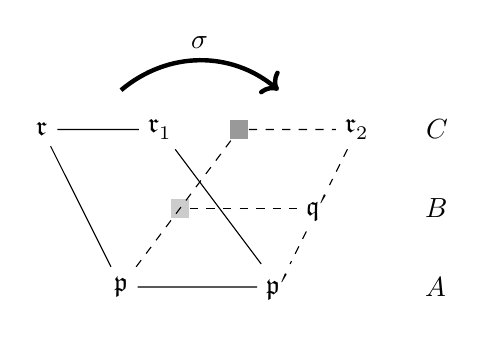
\begin{tikzpicture}
		\node (R) at (-2, 2) {$\mathfrak{r}$};
		\node (R1) at (-0.5, 2) {$\mathfrak{r}_1$};
		\node (R2) at (2, 2) {$\mathfrak{r}_2$};
		\node[fill=gray!80] (SR) at (0.5, 2) {};
		\node[fill=gray!40] (Q) at (-0.25, 1) {};
		\node (Q') at (1.5, 1) {$\mathfrak{q}'$};
		\node (P) at (-1, 0) {$\mathfrak{p}$};
		\node (P') at (1, 0) {$\mathfrak{p}'$};
		
		\node at (3, 2) {$C$}; \node at (3, 1) {$B$}; \node at (3, 0) {$A$};

		\draw (P) -- (R) -- (R1) -- (P') -- (P);
		\draw[dashed] (P) -- (SR) -- (R2) -- (Q')-- (P');
		\draw[dashed] (Q) -- (Q');
		
		\draw (-1, 2.5) edge[->, ultra thick, bend left=40] node[above, midway] {$\sigma$} (1, 2.5);
	\end{tikzpicture}\end{center}
	we first construct $\mathfrak{r}$ and then $\mathfrak{r}_1$ by going-up, then ``tilt'' it via some $\sigma$ to match $\mathfrak{r}_1$ with some chosen $\mathfrak{r}_2$ above $\mathfrak{q}'$, so that $\sigma(\mathfrak{r}) \cap B$ produces the required going-down:
\end{proof}

\begin{exercise}\label{exo:integral-closed}
	Let $A \subset B$ be an integral extension of rings. Show that $\Spec(B) \to \Spec(A)$ is a closed map (Cf.\ Proposition \ref{prop:going-up-closed}.) Hint: Let $\mathfrak{b} \subset B$ be a proper ideal, then $A/\mathfrak{b} \cap A \hookrightarrow B/\mathfrak{b}$ is still integral. Reduce the problem to showing that $V(\{0_B\}) = \Spec(B)$ has closed image in $\Spec(A)$.
\end{exercise}

\section{Subsets in the spectrum}
\begin{proposition}\label{prop:going-up-closed}
	Let $\varphi: A \to B$ be a ring homomorphism with going-up property and suppose $B$ is Noetherian. Then $\varphi^\sharp: \Spec(B) \to \Spec(A)$ is a closed map: it maps closed subsets to closed subsets.
\end{proposition}
\begin{proof}
	Consider a closed subset $V(\mathfrak{b})$ of $\Spec(B)$. First, every $\mathfrak{q} \in \Spec(B)$ with $\mathfrak{q} \supset \mathfrak{b}$ lies over a minimal over-prime of $\mathfrak{b}$, by Lemma \ref{prop:minimal-prime}. Secondly, $B$ is Noetherian implies $\text{Ass}(B/\mathfrak{b})$ is finite; in particular there are only finitely many minimal over-primes $\mathfrak{q}_1, \ldots, \mathfrak{q}_n$ of $\mathfrak{b}$.
	
	Set $\mathfrak{p}_i := \varphi^\sharp(\mathfrak{q}_i)$ for all $i$. By going-up, $V(\mathfrak{p}_i)$ is contained in $\varphi^\sharp(V(\mathfrak{b}))$. On the other hand, every $\mathfrak{p} = \varphi^\sharp(\mathfrak{q})$ with $\mathfrak{q} \in V(\mathfrak{b})$ lies over some $\mathfrak{p}_i = \varphi^\sharp(\mathfrak{q}_i)$ by the foregoing discussion. This shows $\varphi^\sharp(V(\mathfrak{b})) = \bigcup_{i=1}^n V(\mathfrak{p}_i)$ is closed.
\end{proof}

\begin{corollary}
	Suppose $B$ is Noetherian and integral over a subring $A$. Then $\Spec(B) \to \Spec(A)$ is a closed surjection with finite fibers.
\end{corollary}
\begin{proof}
	Apply Theorem \ref{prop:Cohen-Seidenberg} with Proposition \ref{prop:going-up-closed} to show that $\Spec(B) \to \Spec(A)$ is closed and surjective.

	To show the finiteness of the fiber over $\mathfrak{p} \in \Spec(A)$, note that the preimage of $V(\mathfrak{p})$ in $\Spec(B)$ equals $V(\mathfrak{p}B)$. Since there are no inclusions in the fiber over $\mathfrak{p}$, every element in that fiber must be a minimal over-prime of $\mathfrak{p}B$. We have seen in the proof of Proposition \ref{prop:going-up-closed} that there are only finitely many such minimal-over primes.
\end{proof}

Note that the ``closed surjection'' part applies to any integral extension of rings. See Exercise \ref{exo:integral-closed}.

In order to obtain further results of this type, we have to introduce more notions. Let $R$ be a ring.
\begin{definition}
	For $\mathfrak{p}, \mathfrak{p}' \in \Spec(R)$ satisfying $\mathfrak{p} \subset \mathfrak{p}'$, we say $\mathfrak{p}$ is a \emph{generalization} of $\mathfrak{p}'$, and $\mathfrak{p}'$ is a \emph{specialization} of $\mathfrak{p}$.
\end{definition}
To make geometric meaning from it, being ``specialized'' signifies that there are ``more equations'' in $\mathfrak{p}'$, therefore it corresponds a smaller embedded geometric object. For example, in $R=\CC[X,Y]$ the prime ideal $(X,Y)$ is a specialization of $(X)$, as the origin $X=Y=0$ belongs to the line $X=0$.

\begin{lemma}
	With respect to the Zariski topology, $\mathfrak{p}$ is a generalization of $\mathfrak{p}'$ if and only if $\mathfrak{p}' \in \overline{\{\mathfrak{p}\}}$.
\end{lemma}
\begin{proof}
	The condition $\mathfrak{p}' \in \overline{\{\mathfrak{p}\}}$ means that for every ideal $\mathfrak{a}$, if $\mathfrak{p} \supset \mathfrak{a}$ then $\mathfrak{p}' \supset \mathfrak{a}$. Taking $\mathfrak{a} = \mathfrak{p}$ yields $\mathfrak{p}' \supset \mathfrak{p}$, and the converse is even easier.
\end{proof}
A subset is called stable under specialization (resp. generalization) if the specialization (resp. generalization) of any member still belongs to that set. The following is straightforward.

\begin{lemma}\label{prop:stability-vs-closeness-0}
	Any closed subset is stable under specialization; any open subset is stable under generalization.
\end{lemma}

\begin{definition}\index{constructible subset}
	Suppose $R$ is Noetherian. A subset is called \emph{locally closed} if it is the intersection of an open with a closed subset, called \emph{constructible} if it is a finite union of locally closed subsets. % A possibly infinite intersection (resp. union) of constructible subsets is called \emph{pro-constructible} (resp. \emph{ind-constructible}).

	Closed subsets of the form $V(\mathfrak{p})$, where $\mathfrak{p} \in \Spec(R)$, are called \emph{irreducible}; in this case we call $\mathfrak{p}$ the \emph{generic point} of $Z$, which is uniquely characterized as the point which generalizes every member of $Z$.
\end{definition}
\begin{itemize}
	\item The foregoing definition is standard only for $R$ Noetherian. The general definition in EGA differs.
	\item These notions can be applied to any topological space $X$. In practice one usually suppose $X$ to be
		\begin{compactitem}
			\item \emph{Noetherian}: the closed subsets satisfy descending chain condition,
			\item \emph{sober}: every irreducible has a generic point,
		\end{compactitem}
		in order to get interesting results. This explains our Noetherian assumption.
	\item If $\Bbbk$ is algebraically closed, $R = \Bbbk[X_1, \ldots, X_n]/\mathfrak{a}$ corresponds to an affine algebraic variety $\mathcal{X} \subset \Bbbk^n$ and we work with $\MaxSpec(R)$ instead of $\Spec(R)$, then a subset $E \subset \mathcal{X}$ being locally closed means that it can be defined by a formula using the usual language of algebraic operations over $\CC$, with coordinate variables $X_1, \ldots, X_n$  and the symbols $=, \neq$, but \emph{without using the quantifiers $\exists, \forall$}. For example, the formula
	\[ (\neg X = 0) \vee (X = 0 \wedge Y=0) \]
	defines the constructible subset $E := \{(x,y) \in \Bbbk^2 : x \neq 0 \} \cup \{(0,0) \}$, which is neither closed nor open. Note that $E$ is the image of the polynomial map $\Bbbk^2 \to \Bbbk^2$ given by $(x,y) \mapsto (x,xy)$.
\end{itemize}

\begin{exercise}
	Show that the set of constructible subsets is stable under finite $\cup$, finite $\cap$ and taking complements.
\end{exercise}

\begin{exercise}
	Show that irreducible closed subsets $Z$ admit the following topological characterization: if $X = A \cup B$ with $A,B$ closed, then either $X=A$ or $X=B$.
\end{exercise}

Suppose $R$ is Noetherian. Given any closed subset $Z \subset \Spec(R)$, we may write $Z = Z_1 \cup \cdots \cup Z_n$ with each $Z_i$ irreducible. One way to do this is to use the primary decomposition for $\mathfrak{a}$, where we assume $Z = V(\mathfrak{a})$; then $Z_1, \ldots, Z_n$ will correspond to the minimal elements in $\text{Ass}(R/\mathfrak{a})$. One can show by purely topological means that such an irreducible decomposition is unique if we require $i \neq j \implies Z_i \not\subset Z_j$. See \cite[I.1.5]{Har77}.

\begin{lemma}\label{prop:char-constructible}
	Let $E$ be a subset of $\Spec(R)$ where $R$ is a Noetherian ring. The following are equivalent:
	\begin{enumerate}[(i)]
		\item $E$ is constructible;
		\item for every irreducible subset $Z$ of $\Spec(R)$, either $Z \cap E$ is not dense in $Z$ or $Z \cap E$ contains a nonempty open subset of $Z$.
	\end{enumerate}
\end{lemma}
\begin{proof}
	Omitted. See \cite[(6.C)]{Mat80}.
\end{proof}

\begin{theorem}[C.\ Chevalley]\label{prop:Chevalley}\index{Chevalley's theorem}
	Let $\varphi: A \to B$ be a ring homomorphism such that $A$ is Noetherian and $B$ is a finitely generated $A$-algebra. Then $\varphi^\sharp$ maps constructible subsets to constructible subsets.
\end{theorem}
\begin{proof}
	Omitted. See \cite[(6.E)]{Mat80}.
\end{proof}

Now we can give a partial converse to Lemma \ref{prop:stability-vs-closeness-0}, albeit not in the strongest form.
\begin{proposition}
	Suppose $R$ is Noetherian and $E$ is a constructible subset of $\Spec(R)$. If $E$ is stable under specialization (resp. generalization), then $E$ is closed (resp. open) in $\Spec(R)$.
\end{proposition}
\begin{proof}
	It suffices to treat the specialization-stable case by taking complements. Write the Zariski-closure $\bar{E}$ as a finite union of irreducibles components $Z$, without inclusion relations. For each irreducible component $Z$, notice that $Z \cap E$ is dense in $Z$ for all $Z$, since otherwise $\bar{E} = \overline{\bigcup_Z (Z \cap E)} = \bigcup_Z \overline{Z \cap E}$ would lead to another irreducible decomposition. Thus $Z \cap E$ contains a nonempty open of $Z$ by Lemma \ref{prop:char-constructible}. This open subset of $E$ must contain the generic point of $Z$. As $E$ is stable under specialization, we obtain $Z \subset E$. This being true for all $Z$, we deduce that $E = \bar{E}$.
\end{proof}

\begin{proposition}
	Consider a ring homomorphism $\varphi: A \to B$ satisfying going-down. Suppose $A$ is Noetherian and $B$ is a finitely generated $A$-algebra, then $\varphi^\sharp: \Spec(B) \to \Spec(A)$ is an open map.
\end{proposition}
\begin{proof}
	Let $U = \Spec(B) \smallsetminus V(\mathfrak{a})$ be an open subset. Going-down implies that $\varphi^\sharp(U)$ is stable under generalization. It suffices to show $\varphi^\sharp(U)$ is constructible, and this is the content of Chevalley's Theorem \ref{prop:Chevalley}.
\end{proof}

\section{Graded rings and modules}
Let $(\Gamma, +)$ be a commutative monoid. In most cases we consider $\Gamma = \Z_{\geq 0}$.

\begin{definition}\index{graded}
	A $\Gamma$-graded ring is a ring $R$ whose underlying additive group is endowed with a decomposition $R = \bigoplus_{\gamma \in \Gamma} R_\gamma$, such that $R_\gamma R_\eta \subset R_{\gamma + \eta}$ for all $\gamma, \eta \in \Gamma$.
	
	For $R$ as above, a $\Gamma$-graded $R$-module is an $R$-module $M$ whose underlying additive group decomposes as $M = \bigoplus_{\gamma \in \Gamma} M_\gamma$, such that $R_\gamma M_\eta \subset M_{\gamma + \eta}$ for all $\gamma, \eta \in \Gamma$; in particular, $R$ itself is a $\Gamma$-graded $R$-module. If $x \in M_\gamma \smallsetminus \{0\}$, we say $x$ is homogeneous of degree $\gamma$.\index{homogeneous}
\end{definition}
We will often omit $\Gamma$ when there is no worry of confusion. Note that if $0$ is allowed to be homogeneous, as people sometimes do, it will be homogeneous of any degree.

\begin{exercise}
	Show that in a graded ring $R$ we always have $1 \in R_0$, provides that $(\Gamma, +)$ satisfies the cancellation law: $\gamma+\eta=\eta \iff \gamma=0$. Hint: let $e_0$ be the component of $1_R$ in degree 0, argue that $x e_0 = x = e_0 x$ for all homogeneous $x \in R$. The condition $1 \in R_0$ is sometimes built into the definition of graded rings.
\end{exercise}

\begin{definition}
	A graded submodule of a graded $R$-module $M$ is a submodule $N$ with $N = \bigoplus_\gamma (N \cap M_\gamma)$, which gives rise to a natural grading $N_\gamma := N \cap M_\gamma$ on $N$.
\end{definition}
For graded $N \subset M$, the quotient $R$-module $M/N = \bigoplus_\gamma M_\gamma/N_\gamma$ is again graded. As a special case, we have the notion of graded ideals of $R$ (also known as \emph{homogeneous ideals}), and the quotient ring $R/\mathfrak{a}$ with respect to graded $\mathfrak{a}$ inherits the evident grading.

Let $N$ be an $R$-submodule of $M$ and suppose $M$ is graded. The following are easily seen to be equivalent:
\begin{enumerate}[(i)]
	\item $N \subset M$ is graded;
	\item $N$ is generated by homogeneous elements;
	\item if $x = \sum_\gamma x_\gamma \in N$ with each $x_\gamma$ homogeneous of degree $\gamma$, then $\forall \; x_\gamma \in N$.
\end{enumerate}

\begin{example}
	Let $A$ be a ring and $R := A[X_1, \ldots, X_n]$. Then $R$ is naturally $\Z_{\geq 0}$-graded by degrees: for each $d \in \Z_{\geq 0}$, let $R_d$ be the set of homogeneous polynomials of total degree $d$. Ideals generated by homogeneous polynomials are precisely the graded ideals. The importance of this grading comes from projective algebraic geometry.

	On the other hand, $R$ can also be graded by monomials by taking $\Gamma = \Z_{\geq 0} \times \cdots \times \Z_{\geq 0}$ ($n$ copies), and we set $R_{(d_1, \ldots, d_n)} = A \cdot X_1^{d_1} \cdots X_n^{d_n}$
\end{example}

Many constructions in commutative algebra can be generalized to the graded case. Let us illustrate what one can do in an important case, the primary decomposition (cf.\ \cite[\S 3.5 and Exercise 3.5]{Eis95}). In the $\Z$-graded context, it says that for a finitely generated graded module $M$ over a Noetherian graded ring, the associated primes of $M$ are all graded ideals, and one can write $\{0\} = N_1 \cap \cdots \cap N_m$ where $N_i \subset M$ are graded submodules with $\text{Ass}(M/N_i) = \{\mathfrak{p}_i\}$, $\mathfrak{p}_i \in \text{Ass}(M)$, etc. Most of the arguments in the ungraded case carry over verbatim, and the only new technique is the following

\begin{lemma}
	Let $M$ be a $\Z$-graded module over a $\Z$-graded ring $R$. If $x \in M$ and $\mathfrak{p} := \mathrm{ann}(x)$ is a prime ideal, then
	\begin{enumerate}[(i)]
		\item $\mathfrak{p}$ is a homogeneous ideal, and
		\item $\mathfrak{p} = \mathrm{ann}(y)$ for some homogeneous element $y \in M$.
	\end{enumerate}
\end{lemma}
\begin{proof}
	We begin with (i). Let $t \in \mathfrak{p}$ and $x \in M$ be such that $\mathfrak{p} = \text{ann}(M)$. Write
	\[ t = \sum_{\gamma \in \mathcal{A}} t_\gamma, \quad x = \sum_{\eta \in \mathcal{B}} x_\eta, \]
	where $t_\gamma \in R_\gamma \smallsetminus \{0\}$ and $x_\eta \in M_\eta \smallsetminus \{0\}$ for all $\gamma, \eta$. Denote by $\gamma_0$ and $\eta_0$ the minimal elements in $\mathcal{A}$ and $\mathcal{B}$, respectively. Homogenity amounts to $t_\gamma \in \mathfrak{p}$ for each $\gamma \in \mathcal{A}$, and this will be done by induction on $|\mathcal{B}|$. By a further induction on $|\mathcal{A}|$, for fixed $x$ and $\mathfrak{p}$, this can be reduced to showing $t_{\gamma_0} \in \mathfrak{p}$.
	
	First of all, considerations of degrees and $tx=0$ lead to $t_{\gamma_0} x_{\eta_0} = 0$. If $x = x_{\eta_0}$ (i.e.\ $|\mathcal{B}| = 1$), we obtain $t_{\gamma_0} \in \text{ann}(x) = \mathfrak{p}$ as required. In general:
	\begin{itemize}
		\item Suppose that $\mathfrak{p} = \text{ann}(t_{\gamma_0} x)$; since the decomposition
		\[ t_{\gamma_0} x = \sum_{\substack{\eta \in \mathcal{B} \\ \eta \neq \eta_0}} t_{\gamma_0} x_\eta \]
		involves fewer homogeneous terms, $\mathfrak{p}$ is then homogeneous by our induction hypothesis on $|\mathcal{B}|$.
		\item Suppose there exists $s \in R \smallsetminus \mathfrak{p}$ such that $s(t_{\gamma_0} x) = 0$, then $st_{\gamma_0} \in \mathfrak{p}$, hence $t_{\gamma_0} \in \mathfrak{p}$. This concludes the homogeneity (i).
	\end{itemize}
	
	From the homogeneity $\mathfrak{p}$ we infer that $\mathfrak{p} \subset \text{ann}(x_\eta)$ for each $\eta \in \mathcal{B}$. Now that
	\[ \mathfrak{p} = \text{ann}(x) \supset \prod_{\eta \in \mathcal{B}} \text{ann}(x_\eta), \]
	we have $\mathfrak{p} \supset \text{ann}(x_\eta)$ for some $\eta$, hence $\mathfrak{p} = \text{ann}(x_\eta)$. Take $y = x_\eta$ to obtain (ii).
\end{proof}

\section{Filtrations}
Now turn to filtrations. We only deal with decreasing filtrations indexed by $\Z_{\geq 0}$.
\begin{definition}\index{filtration}\index{gr@$\gr_F(M)$}
	A \emph{filtration} on a ring $R$ is a descending sequence
	\[ R = F^0 R \supset F^1 R \supset F^2 R \supset \cdots \]
	of ideals such that $F^i R \cdot F^j R \subset F^{i+j} R$. Define the associated $\Z_{\geq 0}$-graded ring
	\[ \gr_F(R) := \bigoplus_{n \geq 0} \underbracket{F^n R \big/ F^{n+1} R}_{=: \gr_F^n R} \]
	whose multiplication is defined as follows: if $x \in F^n R / F^{n+1} R$ and $y \in F^m R/F^{m+1} R$, choose liftings $\tilde{x} \in F^n R$ and $\tilde{y} \in F^m R$ and define
	\[ xy := \text{the image of }\; \tilde{x}\tilde{y}\; \text{ in }\; F^{n+m} R / F^{n+m+1} R; \]
	this is readily seen to be well-defined. The multiplication of arbitrarily many homogeneous elements can be obtained in the same recipe. The datum $(R, F^\bullet R)$ is called a \emph{filtered ring},

	Given a filtered ring $R$, a \emph{filtered $R$-module} $M$ is an $R$-module $M$ equipped with a descending sequence\footnote{In view of later applications, the filtration on a module is indexed by $\Z$ instead of $\Z_{\geq 0}$.} of submodules
	\[ \cdots \supset F^i M \supset F^{i+1} M \supset \cdots, \quad i \in \Z \]
	such that $F^i R \cdot F^j M \subset F^{i+j} M$. Define the associated graded module as the $\Z$-graded $\gr_F R$-module
	\[ \gr_F(M) := \bigoplus_{n \in \Z} \underbracket{F^n M \big/ F^{n+1} M}_{=: \gr_F^i M} \]
	whose scalar multiplication is defined using liftings as above.
\end{definition}

The subscript $F$ in $\gr$ will often be omitted. To guarantee that $\gr_F(R) \neq \{0\}$, we usually impose the harmless condition
\[ R = F^0 R \supsetneq F^1 R. \]

\begin{example}\index{filtration!$\mathfrak{a}$-adic}
	Let $\mathfrak{a}$ be a proper ideal of $R$, then $F^i R := \mathfrak{a}^i$ defines a filtration on $R$, called the \emph{$\mathfrak{a}$-adic filtration}.
\end{example}

\begin{definition}\label{def:a-stable}
	Equip $R$ with the $\mathfrak{a}$-adic filtration. A filtered $R$-module $M$ is called $\mathfrak{a}$-\emph{stable} if $\mathfrak{a} \cdot F^i M = F^{i+1} M$ for $i \gg 0$.
\end{definition}
Recall that $\mathfrak{a} \cdot F^i M \subset F^{i+1} M$ holds for all $M$, which is a part of our assumption.

As an easy example, set $F^i M := \mathfrak{a}^i M$ for $i \geq 1$, and $F^{\leq 0} M := M$; this is the $\mathfrak{a}$-adic filtration on $M$, which is obviously $\mathfrak{a}$-stable.

\begin{proposition}\label{prop:gr-Noetherian}
	Suppose $\mathfrak{a}$ is a proper ideal of $R$. If $R$ is Noetherian, so is $\gr(R)$ with respect to the $\mathfrak{a}$-adic filtration. In fact $\gr(R)$ is finitely generated over $\gr^0(R)$.
\end{proposition}
\begin{proof}
	Let $x_1, \ldots, x_n$ be generators of $\mathfrak{a}$, with images $\bar{x}_i \in \mathfrak{a}/\mathfrak{a}^2$. Then $\gr(R)$ is generated by $\bar{x}_1, \ldots \bar{x}_n$ over $R/\mathfrak{a} = \gr^0 R$, which is also Noetherian. Now apply Hilbert's Basissatz.
\end{proof}

\begin{proposition}\label{prop:gr-fg}
	Let $\mathfrak{a}$ be a proper ideal of $R$ and $M$ a finitely generated $R$-module. Suppose $M$ is endowed with an $\mathfrak{a}$-stable filtration such that $F^i M$ is finitely generated for each $i$, and $F^{\leq 0} M = M$. Then $\gr(M)$ is a finitely generated $\gr(R)$-module.
\end{proposition}
\begin{proof}
	Take $n$ such that $\mathfrak{a} \cdot F^i M = F^{i+1} M$ for all $i \geq n$. Then in $\gr(M) = \bigoplus_i \gr^i M$ we have
	\[ (\mathfrak{a}/\mathfrak{a}^2) \cdot \gr^i M = \gr^{i+1} M, \quad i \geq n. \]
	Therefore it suffices to take generators from $\gr^0 M, \ldots, \gr^n M$, each of whom is finitely generated over $R/\mathfrak{a} = \gr^0 R$.
\end{proof}

\section{Theorems of Artin--Rees and Krull}\label{sec:Artin-Rees}
Conserve the conventions in the previous section on filtrations, etc.

\begin{definition}[Morphisms between filtered objects]
	Let $(A, F^\bullet A)$ and $(B, F^\bullet B)$ be filtered rings. A \emph{morphism} between them means a ring homomorphism $\varphi: A \to B$ satisfying $\varphi(F^i A) \subset F^i B$ for all $i$. Similarly, suppose $A$ is filtered and let $M, N$ be filtered $A$-modules. A morphism $M \to N$ means a homomorphism $\psi: M \to N$ of $R$-modules satisfying $\psi(F^i M) \subset F^i N$ for all $i$.
\end{definition}
This makes the filtered rings and the filtered modules over a filtered ring into categories. Obviously, morphisms $\varphi$ between filtered objects induce graded morphisms $\gr \varphi$ between the associated graded objects. Therefore we obtain a functor from the category of filtered rings or modules into their graded avatars.

\begin{remark}
	Suppose $\varphi: M \to N$ is a morphism between filtered $A$-modules. The quotient $M/\Ker(\varphi)$ inherits a filtration from $M$, whereas the submodule $\Image(\varphi)$ inherits one from $N$. When the natural isomorphism $M/\Ker(\varphi) \to \Image(\varphi)$ is an isomorphism between filtered modules, or equivalently
	\[ \forall i \in \Z, \; \varphi(F^i M) = \varphi(M) \cap F^i N, \]
	we say $\varphi$ is a \emph{strict morphism}.
\end{remark}

It is often useful to relate properties of a filtered module or morphism to its graded counterpart. Propositions \ref{prop:gr-Noetherian} and \ref{prop:gr-fg} are such examples. Here is an example for the other direction. We say that a filtration on $M$ is \emph{exhaustive} if $\bigcup_i F^i M = M$, \emph{separating} (or \emph{Hausdorff}) if $\bigcap_i F^i M = \{0\}$

\begin{proposition}\label{prop:gr-injective}
	Suppose that $\varphi: M \to N$ is a morphism between filtered $R$-modules. If $M$ is exhaustive and separating, and $\gr\varphi$ is injective, then $\varphi$ is also injective.
\end{proposition}
\begin{proof}
	Let $x \in \Ker(\varphi)$. There exists $n$ such that $x \in F^n M$. Regard $x + F^{n+1} M$ as an element of $\gr^n M$. Then $\gr(\varphi)(x + F^{n+1} M) = \varphi(x) + F^{n+1} N = 0$, so $x \in F^{n+1} M$. Iterating this argument, we have $x \in \bigcap_{k \geq n} F^k M = \{0\}$.
\end{proof}
See Lemma \ref{prop:gr-surjective} for the case of surjections.

In what follows, $\mathfrak{a}$ always denotes a proper ideal of a ring $R$.

\begin{definition}[Blow-up algebras and modules]\index{blow-up algebra}
	Introduce an indeterminate $X$ and define the $\Z_{\geq 0}$-graded $R$-algebra
	\[ \text{Bl}_{\mathfrak{a}} R := \bigoplus_{n \geq 0} \mathfrak{a}^n X^n \; \subset R[X]. \]
	If an $R$-module $M$ is endowed with a filtration $(F^i M)_{i \geq 0}$ compatible with $\mathfrak{a}$, we define
	\[ \text{Bl}(M) := \bigoplus_{n \geq 0} (F^n M) \otimes X^n \subset M \dotimes{R} R[X]. \]
	Clearly, $\text{Bl}(M)$ is a graded $\text{Bl}_{\mathfrak{a}} R$-module.
\end{definition}

\begin{remark}
	The indeterminate $X$ is somehow a placeholder. Enlarge $\text{Bl}_{\mathfrak{a}} R$ to $\tilde{B}$ by setting the negative graded pieces to be $R \cdot X^{< 0}$, and set $T = X^{-1}$. We see that $\tilde{B}$ is actually an $R[T]$-algebra, sometimes called the \emph{Rees algebra} of $\mathfrak{a}$. Under the specialization $T=0$ we get \index{Rees algebra}
	\[ \frac{ \tilde{B}}{T \tilde{B}} \simeq \bigoplus_{n \geq 0} \frac{\mathfrak{a}^n}{\mathfrak{a}^{n+1}} \cdot T^{-n} \simeq \gr(R). \]
	On the other hand, inverting $T$ yields
	\[ \tilde{B}[T^{-1}] = \bigoplus_{n \in \Z} R \cdot T^{-n} = R[T^{\pm 1}]. \]
	This reflects a well-known deformation construction in geometry; $\gr(R)$ is actually the graded $R$-algebra corresponding to the \emph{normal cone} defined by $\mathfrak{a} \subset R$. We refer to \cite[\S 5.1]{Fu98} for details.
\end{remark}

\begin{lemma}\label{prop:Bl-fg}
	Consider a ring $R$ with proper ideal $\mathfrak{a}$, together with a filtered $R$-module $M$, assume furthermore that each $F^i M$ is finitely generated over $R$. The following are equivalent:
	\begin{enumerate}[(i)]
		\item $\mathrm{Bl}(M)$ is finitely generated over $\mathrm{Bl}_{\mathfrak{a}} R$;
		\item the filtration on $M$ is $\mathfrak{a}$-stable. (Definition \ref{def:a-stable})
	\end{enumerate}
\end{lemma}
\begin{proof}
	(i) $\implies$ (ii): Choose homogeneous generators $x_1, \ldots, x_n \in \text{Bl}(M)$ with degrees $d_1, \ldots, d_n$ respectively. It is then routine to see that
	\[ i \geq \max\{d_1, \ldots, d_n \} \implies (F^{i+1} M) X^{i+1} = \mathfrak{a} X \cdot (F^i M) X^i, \]
	that is, $\mathfrak{a} \cdot F^i M = F^{i+1} M$ for these $i$.

	(ii) $\implies$ (i): Suppose $\mathfrak{a} \cdot F^i M = F^{i+1} M$ for $i \geq d$, then $\text{Bl}(M)$ is generated by $\bigoplus_{j \leq d} (F^j M) X^j$, and each $F^j M$ is finitely generated over $R = (\text{Bl}_{\mathfrak{a}} R)_0$.
\end{proof}

\begin{theorem}[Artin--Rees]\label{prop:Artin-Rees}
	Let $R$ be a Noetherian ring endowed with $\mathfrak{a}$-adic filtration. Let $M$ be a finitely generated $R$-module and $N \subset M$ an $R$-submodule. Then the filtration on $N$ induced by the $\mathfrak{a}$-adic filtration of $M$, namely $F^i N := \mathfrak{a}^i M \cap N$, is $\mathfrak{a}$-stable.
\end{theorem}
\begin{proof}
	Define $\text{Bl}(N)$ using the induced filtration $F^i N := \mathfrak{a}^i M \cap N$, which is a submodule of the finitely generated $\text{Bl}_{\mathfrak{a}} R$-module $\text{Bl}(M)$ (Lemma \ref{prop:Bl-fg}). If $\mathfrak{a} = (a_1, \ldots, a_m)$ than $\text{Bl}_{\mathfrak{a}} R = R[a_1 X, \ldots, a_m X] \subset R[X]$, hence Noetherian by Hilbert's Basissatz. We deduce that $\text{Bl}(N)$ is finitely generated over $\text{Bl}_{\mathfrak{a}} R$. In turn, this implies $F^\bullet N$ is an $\mathfrak{a}$-stable filtration on $N$ by Lemma \ref{prop:Bl-fg}.
\end{proof}

\begin{theorem}\label{prop:intersection-thm}
	For $R, \mathfrak{a}, M$ as in the previous theorem, we set $N := \bigcap_{n \geq 0} \mathfrak{a}^n M$. Then $\mathfrak{a}N = N$.
\end{theorem}
\begin{proof}
	Since the induced filtration on $N$ is $\mathfrak{a}$-stable by Theorem \ref{prop:Artin-Rees}, for $n \gg 0$ we have
	\[ N = \mathfrak{a}^n M \cap N = \mathfrak{a} \cdot (\mathfrak{a}^{n-1} M \cap N) = \mathfrak{a} N. \]
	The assertion follows.
\end{proof}

\begin{corollary}[Krull]\label{prop:Krull-intersection-rad}
	If $\mathfrak{a} \subset \mathrm{rad}(R)$, then $\bigcap_{n \geq 0} \mathfrak{a}^n M = \{0\}$ for any finitely generated $R$-module $M$. In particular $\bigcap_{n \geq 0} \mathfrak{a}^n = \{0\}$ whenever $\mathfrak{a} \subset \mathrm{rad}(R)$.
\end{corollary}
\begin{proof}
	Theorem \ref{prop:intersection-thm} together with Nakayama's lemma imply $N = \{0\}$.
\end{proof}

\begin{corollary}[Krull's Intersection Theorem]\label{prop:Krull-intersection-domain}\index{Krull's intersection theorem}
	Let $R$ be a Noetherian domain and $\mathfrak{a}$ a proper ideal. Then $\bigcap_{n \geq 0} \mathfrak{a}^n = \{0\}$.
\end{corollary}
\begin{proof}
	Define $N := \bigcap_{n \geq 0} \mathfrak{a}^n \subset R$. By Theorem \ref{prop:intersection-thm} we have $\mathfrak{a}N = N$, thus there exists $r \in \mathfrak{a}$ with $1+r \in \text{ann}(N)$ by Nakayama's Lemma (Theorem \ref{prop:NAK}). As $\mathfrak{a}$ is proper, $1+r$ cannot be zero. Since $R$ is a domain containing $N$, the only possibility is $N=\{0\}$ as asserted.
\end{proof}
	% To be compiled by XeLaTeX, preferably under TeX Live.
% LaTeX source for ``Yanqi Lake Lectures on Algebra'' Part III.
% Copyright 2019  李文威 (Wen-Wei Li).
% Permission is granted to copy, distribute and/or modify this
% document under the terms of the Creative Commons
% Attribution-NonCommercial 4.0 International (CC BY-NC 4.0)
% https://creativecommons.org/licenses/by-nc/4.0/

% To be included
\chapter{From completions to dimensions}

The main references are \cite{Mat80,Eis95}.
\section{Completions}
Consider a ring $R$ together with a family of ideals $\mathcal{I} \neq \emptyset$, such that for any $I, J \in \mathcal{I}$ there exists $K \in \mathcal{I}$ with $K \subset I \cap J$. This turns $R$ into a topological ring, characterized by the property that $\mathcal{I}$ forms a local base of open neighborhoods of $0$. Recall that being a topological ring means that addition, multiplication and $x \mapsto -x$ are all continuous. By standard arguments, $R$ is Hausdorff if and only if $\{0\}$ is closed, if and only if $\bigcap_{I \in \mathcal{I}} I = \{0\}$.\index{topological ring}

To simplify matters, we assume that
\begin{compactitem}
	\item the family $\mathcal{I}$ is countable, so that the topological properties (accumulation points, etc.) are detected by convergence of \emph{sequences} as in the case of metric spaces;
	\item furthermore, we may arrange that $\mathcal{I} = \{I \supset J \supset K \supset \cdots \}$, in other words our topology comes from \emph{filtrations}.
\end{compactitem}
Without the countability assumption, the sequences will have to be replaced by \emph{filters}.

It makes sense to talk about topological $R$-modules for a topological ring $R$. By replacing filtration by ideals by filtration by $R$-submodules subject to the usual compatibility relation $F^i R \cdot F^j M \subset F^{i+j} M$, the recipe above applies to $R$-modules as well. Given $N \subset M$, the topology so obtained on $M$ passes to $M/N$ by taking the quotient topology, or equivalently the quotient filtration $(F^\bullet M+N)/N$. If the filtration in question is $I$-adic, where $I \subsetneq R$ is an ideal, we obtain the \emph{$I$-adic topology} on rings and modules.\index{topological ring!$I$-adic}

An $R$-module $M$ equipped with a topology as above is \emph{complete} if every Cauchy sequence $(x_n)_{n \geq 1}$ has a limit; a Cauchy sequence $(x_n)_{n \geq 1}$ is a sequence satisfying
\[ \forall I \in \mathcal{I}, \; \exists N \quad i,j \geq N \implies x_i - x_j \in I. \]
As in the familiar case of metric spaces, one has the \emph{completion} of $M$. It is actually a morphism $M \to \hat{M}$ with $\hat{M}$ complete Hausdorff, characterized by the following universal property:\index{completion}
\[
\begin{tikzcd}[row sep=tiny, column sep=tiny]
	M \arrow[rr, "\varphi:\; \text{cont. homo.}" inner sep=0.7em] & & L \\
	& & \scriptsize\text{complete Hausdorff}
\end{tikzcd} \quad \leadsto
\begin{tikzcd}
	M \arrow[rd, "\varphi"'] \arrow[r] & \hat{M} \arrow[dashed, d, "\exists! \hat{\varphi}"] \\
	& L
\end{tikzcd}\]

The uniqueness results immediately, and the formation of $M \mapsto \hat{M}$ is seen to be functorial in $M$. If $M$ is already complete Hausdorff, one may take $\hat{M} = M$. Certainly, the same applies to the ring $R$.

\begin{exercise}
	Suppose that $R$ is complete Hausdorff with respect to the $I$-adic topology, where $I$ is a proper ideal. Show that every element of the form $u+x$, $u \in R^\times$ and $x \in I$, is invertible.
\end{exercise}

From the algebraic perspective, the completion of a filtered $R$-module $M = F^0 M \supset F^1 M \supset \cdots$ can be constructed as the projective limit
\begin{align*}
	\hat{M} & := \varprojlim_{i \geq 1} M/F^i M \\
	& = \left\{ (x_i)_{i \geq 1} : i \leq j \implies x_i \equiv x_j \pmod{F^i M} \right\} \subset \prod_{i \geq 1} M/F^i M.
\end{align*}
The morphism $M \to \hat{M}$ is the diagonal map. The topology on $\hat{M}$ arises from the filtration
\[ F^i \hat{M} := \Ker\left[ p_i: \hat{M} \to M/F^i M \right] = \left\{ (x_n)_n \in \hat{M}: i \leq k \implies x_i=0 \right\}, \]
so that the preimage of $F^i \hat{M}$ in $M$ is precisely $F^i M$. In the case where $M=R$ and $F^i R$ are ideals, we obtain the complete Hausdorff ring $\hat{R}$, which is a subring of $\prod_{i \geq 1} R/F^i R$. Since the filtrations on $R$ and $M$ are assumed compatible, $\hat{M}$ is an $\hat{R}$-module.

\begin{example}
	Fix a prime number $p$. The completion of $\Z$ with respect to the ideal $p\Z$ is nothing but the ring $\Z_p$ of $p$-adic integers. Similarly, the completion of $\Bbbk[X]$ with respect to $(X)$ is isomorphic to the $\Bbbk$-algebra $\Bbbk\llbracket X\rrbracket$.
\end{example}

\begin{exercise}
	Describe the kernel of $M \to \hat{M}$ and show $M \hookrightarrow \hat{M}$ if and only if $M$ is Hausdorff.
\end{exercise}

\begin{exercise}
	Show that the topology of $\hat{M}$ is the restriction of the product topology of $\prod_i M/F^i M$, provided that each $M/F^i M$ is endowed with the discrete topology. Show that $\hat{M}$ is a closed subspace of $\prod_i M/F^i M$
\end{exercise}

\begin{lemma}\label{prop:quotient-completion}
	Let $M$ be a complete $R$-module with respect to some filtration $F^\bullet M$. For any submodule $N$, the quotient $M/N$ is also complete with respect to the quotient topology, or equivalently with respect to the quotient filtration $(F^\bullet M + N)/N$.
\end{lemma}
\begin{proof}
	Let $\bar{x}_n$ be a Cauchy sequence in $M/N$. Choose preimages $M \ni x_n \mapsto \bar{x}_n$ for all $n$. We have $\bar{x}_{n+1} - \bar{x}_n \in F^{i(n)}M + N$ where $\lim_{n \to \infty} i(n) = \infty$, therefore we can write $x_{n+1} - x_n = y_n + \delta_n$ where $y_n \in F^{i(n)} M$ and $\delta_n \in N$. We contend that $x'_n := x_1 + \sum_{i < n} y_i$ is a Cauchy sequence in $M$. Indeed, for any $i > j$ we have $x'_i - x'_j = \sum_{j \leq k < i} y_k$, which lies in $F^{\inf_k i(k)} M$. This implies $(x'_n)_n$ is a Cauchy sequence, hence has a limit $x \in M$. It is also clear that $x'_n \mapsto \bar{x}_n$. Hence $\bar{x}'_n$ has a limit $\bar{x} = x \bmod N$ in $M/N$.
\end{proof}

Let us turn to the exactness of completion. This should be understood in the broader framework of $\varprojlim$ of arbitrary projective systems. For simplicity, we only consider $I$-adic topologies on finitely generated modules over a Noetherian ring.

Observe that any homomorphism $\varphi: M \to N$ between $R$-modules is automatically $\mathfrak{a}$-adically continuous, for that $\varphi(\mathfrak{a}^n M) \subset \mathfrak{a}^n N$.

\begin{proposition}\label{prop:completion-exactness}
	Let $R$ be a Noetherian ring and $I \subsetneq R$ an ideal. Suppose $0 \to M' \to M \to M'' \to 0$ is an exact sequence of finitely generated $R$-modules, each term equipped with the $I$-adic topology. The completed sequence $0 \to \hat{M}' \to \hat{M} \to \hat{M''} \to 0$ is also exact.
\end{proposition}
Consequently, completion preserves the exactness of sequences formed by finitely generated $R$-modules. This is what makes completion so useful.
\begin{proof}
	We shall show
	\begin{compactenum}[(i)]
		\item the topology on $M'$ induced from $M$ is the same as the $I$-adic topology;
		\item the quotient topology on $M'' = M/M'$ is $I$-adic;
		\item the completion $\hat{M}'$ is naturally identified with the closure of the image of $M'$ in $\hat{M}$;
		\item $\hat{M}''$ is naturally identified with the quotient of $\hat{M}$ by $\hat{M}'$.
	\end{compactenum}

	(i) is a direct consequence of Artin--Rees Theorem \ref{prop:Artin-Rees}: for $n \gg 0$ we have
	\begin{gather}\label{eqn:AR-induced-top}
		I^n M' \subset M' \cap I^n M = I (M' \cap I^{n-1} M) \subset I^{n-1} M',
	\end{gather}
	and this suffices to identify the resulting topologies.
	
	(ii) is immediate. As for (iii), we may embed $M'$ into $M$ and work with the induced topology. Realize $\hat{M}$ as $\varprojlim_n M/I^n M$. As a topological module $\hat{M}'$ equals
	\begin{align*}
		\varprojlim_n \frac{M'}{M' \cap I^n M} & = \left\{ \hat{x} = (x_n)_n \in \hat{M} : \forall k, \; x_k \text{ comes from } M' \right\} \\
		& = \left\{ \hat{x} \in \hat{M}: \forall k \; \exists y \in M' \text{ s.t. } \; \hat{x} \in y + F^k \hat{M} \right\}
	\end{align*}
	which is readily seen to be the closure of the image of $M'$.
	
	For (iv), the quotient $\hat{M}/\hat{M}'$ is Hausdorff since $\hat{M}'$ is a closed submodule. It is also complete by Lemma \ref{prop:quotient-completion}. There is a natural homomorphism $M/M' \to \hat{M}/\hat{M}'$. Given any continuous homomorphism $\varphi: M/M' \to N$ to a complete Hausdorff $R$-module $N$, we may pull it back to $M \to N$, which corresponds to a unique continuous $\hat{M} \to N$ that is trivial on the image of $M'$; but such a homomorphism must also vanish on the closure $\hat{M}'$. This yields the required $\hat{\varphi}: \hat{M}/\hat{M}' \to N$ in the universal property.
\end{proof}

For any $R$-module $M$ endowed with $I$-adic topology, there is a canonical homomorphism $M \dotimes{R} \hat{R} \to \hat{M}$. Indeed, $\hat{M} = \varprojlim_n M/I^n M$ is a $\hat{R} = \varprojlim_n R/I^n$-module by
\[ (r_n)_{n \geq 1} \cdot (x_n)_{n \geq 1} = (r_n x_n)_{n \geq 1}, \quad (r_n)_n \in \hat{R}, \; (x_n)_n \in \hat{M}, \]
hence the $R$-homomorphism $M \to \hat{M}$ gives rise to $M \dotimes{R} \hat{R} \to \hat{M}$ by the universal property of base change. This homomorphism is continuous if $M \dotimes{R} \hat{R}$ is filtered by the images of $M \dotimes{R} (F^\bullet \hat{R})$, which makes it into a topological $\hat{R}$-module.

\begin{theorem}\label{prop:completion-tensor}
	Suppose $R$ is Noetherian. Let $M$ be a finitely generated $R$-module endowed with the $I$-adic topology. The homomorphism $M \dotimes{R} \hat{R} \to \hat{M}$ is then an isomorphism.
\end{theorem}
\begin{proof}
	Write down a finite presentation $R^{\oplus a} \to R^{\oplus b} \to M \to 0$. By the naturality of the homomorphism above, the right-exactness of $\otimes$ and Proposition \ref{prop:completion-exactness}, we have a commutative diagram
	\[\begin{tikzcd}
		R^{\oplus a} \dotimes{R} \hat{R} \arrow[r] \arrow[d] & R^{\oplus a} \dotimes{R} \hat{R} \arrow[r] \arrow[d] & M \dotimes{R} \hat{R} \arrow[r] \arrow[d] & 0 \\
		\widehat{R^{\oplus a}} \arrow[r] & \widehat{R^{\oplus b}} \arrow[r] & \hat{M} \arrow[r] & 0
	\end{tikzcd}\]
	with exact rows. Completion commutes with direct sums: $(N_1 \oplus N_2)^\wedge = \hat{N}_1 \oplus \hat{N}_2$ canonically (easy, and the categorical reason is that completion is left adjoint to oblivion $R\dcate{CompHausMod} \to R\dcate{TopMod}$). Therefore the first two vertical arrows may be identified with the canonical arrow $R^{\oplus \star} \dotimes{R} \hat{R} \to \hat{R}^{\oplus \star}$, $\star \in \{a,b\}$, which is an isomorphism of topological $\hat{R}$-modules. We infer that $M \dotimes{R} \hat{R} \rightiso \hat{M}$ topologically.
\end{proof}
\begin{remark}
	In fact $M \dotimes{R} \hat{R} \rightiso \hat{M}$ is also a homeomorphism. It suffices to observe that in the rows of the commutative diagram above, $M \dotimes{R} \hat{R}$ and $\hat{M}$ are both realized as quotient topological $\hat{R}$-modules, and that $R^{\oplus \star} \dotimes{R} \hat{R} \rightiso \hat{R}^{\oplus \star}$ is a homeomorphism. The second point has been observed in the proof of Proposition \ref{prop:completion-exactness}, and the first follows from the fact completed modules carry the $\hat{I}$-adic topology. See Proposition \ref{prop:completion-top}. We do not need this result.
\end{remark}

In the following statements, $R$ is Noetherian and an ideal $I \subsetneq R$ is chosen.
\begin{corollary}
	The canonical homomorphism $R \to \hat{R}$ is flat.
\end{corollary}
\begin{proof}
	Flatness can be tested on short exact sequences of the form $0 \to \mathfrak{a} \to R \to R/\mathfrak{a} \to 0$ where $\mathfrak{a}$ is a finitely generated ideal of $R$. Its base-change to $\hat{R}$ is the same as completion, and completion is an exact functor by Proposition \ref{prop:completion-exactness}.
\end{proof}

\begin{corollary}\label{prop:completion-auto}
	Assume $R$ is $I$-adically complete Hausdorff. Then every finitely generated $R$-module $M$ is $I$-adically complete Hausdorff, and any submodule $N \subset M$ is closed.
\end{corollary}
\begin{proof}
	For the first assertion: the completion of $M$ can be identified with the composite $M = M \dotimes{R} R \to M \dotimes{R} \hat{R} \to \hat{M}$, which is bijective. Therefore every Cauchy sequence in $M$ has a limit in $M$.

	As to the second assertion, recall that the $I$-adic topology on $N$ is the same as the one restricted from $M$ by \eqref{eqn:AR-induced-top}. It remains to notice that complete subspaces must be closed.
\end{proof}

\section{Further properties of completion}
Let $R$ be a Noetherian ring and $M$ a finitely generated $R$-module. Fix an ideal $I \subsetneq R$. Unless otherwise specified, the topologies and completions are always $I$-adic.

\begin{proposition}\label{prop:completion-aux}
	Let $\mathfrak{a}$ be an ideal, then $\mathfrak{a} \hat{M} = \widehat{\mathfrak{a}M} = \hat{\mathfrak{a}}\hat{M}$ as submodules of $\hat{M}$. Consequently $\hat{M}/\mathfrak{a}\hat{M} \simeq (M/\mathfrak{a}M)^\wedge$ canonically.
\end{proposition}
\begin{proof}
	By the exactness of completion (Proposition \ref{prop:completion-exactness}), we may realize $\hat{\mathfrak{a}}$ as an ideal of $\hat{R}$; in fact it is the image $\mathfrak{a} \hat{R}$ of $\mathfrak{a} \dotimes{R} \hat{R} \to R \dotimes{R} \hat{R} = \hat{R}$. Hence $\mathfrak{a}\hat{R} = \hat{\mathfrak{a}}$. Now consider the commutative diagram
	\[\begin{tikzcd}
		\mathfrak{a} \dotimes{R} M \dotimes{R} \hat{R} \arrow[r] \arrow[rd] \arrow[twoheadrightarrow, d] & \mathfrak{a} \dotimes{R} \hat{M} \arrow[d] \\
		\mathfrak{a}M \dotimes{R} \hat{R} \arrow[r] & \hat{M}
	\end{tikzcd}\]
	The upper horizontal arrow is an isomorphism by Theorem \ref{prop:completion-tensor}, therefore the diagonal arrow has image equal to $\mathfrak{a}\hat{M}$. The lower horizontal arrow is just the completion of $\mathfrak{a}M \hookrightarrow M$, thus injective with image $(\mathfrak{a}M)^\wedge$ by Proposition \ref{prop:completion-exactness}. A comparison yields $(\mathfrak{a}M)^\wedge = \mathfrak{a}\hat{M}$. Also note that $\hat{\mathfrak{a}}\hat{M} = \mathfrak{a}\hat{R}\hat{M} = \mathfrak{a}\hat{M}$. The final assertion results from the exactness of completion.
\end{proof}
Since the $I$-adic topology on $M/I^n M$ is discrete, as a special case ($\mathfrak{a} = I^n$) we deduce the natural identifications
\begin{gather*}
	M/I^n M = \hat{M}/I^n \hat{M} = \hat{M}/\hat{I}^n \hat{M}, \quad \forall n \geq 0, \\
	\gr_I(R) = \gr_I(\hat{R}) = \gr_{\hat{I}}(\hat{R}), \\
	\gr_I(M) = \gr_I(\hat{M}) = \gr_{\hat{I}}(\hat{M}).
\end{gather*}

\begin{proposition}\label{prop:completion-top}
	For any finitely generated $R$-module $M$, the topology on $\hat{M}$ coincides with the $\hat{I}$-adic one.
\end{proposition}
\begin{proof}
	Consider the closure of the image of $I^n M$ in $\hat{M}$. It is readily seen to be $\{(x_k)_k: i \leq n \implies x_i=0 \} = F^n \hat{M}$. On the other hand, we have seen that this closure is $\widehat{I^n M} \subset \hat{M}$. By virtue of Proposition \ref{prop:completion-aux}, we have $\widehat{I^n M} = \widehat{I^n}\hat{M}$ and $\widehat{I^n} = I^n \hat{R} = (I\hat{R})^n = \hat{I}^n$.
\end{proof}

\begin{lemma}\label{prop:gr-surjective}
	Consider a homomorphism $\varphi: L \to N$ between filtered modules over some ring, such that $L$ is complete, $N$ is Hausdorff and exhaustive (see \S\ref{sec:Artin-Rees}) with respect to their filtrations, and $\gr(\varphi): \gr(L) \to \gr(N)$ is surjective. Then $\varphi$ is also surjective.
\end{lemma}
\begin{proof}
	Let $y \in F^d N$, we may take $x \in F^d L$ such that $y' := y- \varphi(x) \in F^{d+1} N$. Next, take $x' \in F^{d+1} L$ with $y'' := y' -  \varphi(x') \in F^{d+2} N$, and so forth. Use the completeness of $L$ to define $x_\infty := x + x' + x'' + \cdots$, which maps to $y$ since $N$ is Hausdorff.
\end{proof}

\begin{proposition}\label{prop:completion-rad}
	The ring $\hat{R}$ is also Noetherian, and $\hat{I} \subset \mathrm{rad}(\hat{R})$.
\end{proposition}
\begin{proof}
	Let $\mathfrak{A}$ be any ideal of $\hat{R}$, equipped with the filtration $F^n \mathfrak{A} := \hat{I}^n \cap \mathfrak{A}$. We have to show $\mathfrak{A}$ is finitely generated. Since $\gr_I(R) = \gr_{\hat{I}}(\hat{R})$ is Noetherian, so is $\gr_F(\mathfrak{A})$. Take $t_1, \ldots, t_n \in \mathfrak{A}$, $t_i \in F^{d_i} \mathfrak{A}$, whose images $\bar{t}_i$ in $\gr^{d_i}_F(\mathfrak{A})$ generates $\gr_F(\mathfrak{A})$. Using an appropriately shifted filtration on $L := \hat{R}^{\oplus n}$, we obtain a filtered homomorphism $\varphi: L \to  \mathfrak{A}$ with image $(t_1, \ldots, t_n)$, such that $\gr(\varphi)$ is surjective. Now apply the previous Lemma to obtain the first assertion.
	
	One of the characterizations of Jacobson radical says that $\hat{I} \subset \mathrm{rad}(\hat{R})$ if and only if $1 - \hat{I} \subset \hat{R}^\times$. This is verified by noting that $(1-t)^{-1} = 1+t+t^2+ \cdots$ converges $I$-adically. This proves the second assertion.
\end{proof}

\begin{proposition}\label{prop:completion-semilocal}
	The map $\mathfrak{p} \mapsto \hat{\mathfrak{p}}$ furnishes an injection from $V(I)$ to $\Spec(\hat{R})$ satisfying $R/\mathfrak{p} \simeq \hat{R}/\hat{\mathfrak{p}}$ (as rings). It restricts to a bijection $\MaxSpec(R) \cap V(I) \xrightarrow{1:1} \MaxSpec(\hat{R})$.

	Consequently, if $R$ is local (resp. semi-local), so is $\hat{R}$.
\end{proposition}
\begin{proof}
	Since $\mathfrak{p} \supset I$, the $I$-adic topology on $R/\mathfrak{p}$ is discrete. By Proposition \ref{prop:completion-aux}, $\hat{R}/\hat{p} \simeq (R/\mathfrak{p})^\wedge = R/\mathfrak{p}$, and here the isomorphism even respects ring structures. Therefore $\hat{\mathfrak{p}}$ is a prime ideal. Moreover, it is maximal if and only if $\mathfrak{p}$ is. Claim: $\mathfrak{p}$ is the preimage of $\hat{\mathfrak{p}} = \varprojlim_n \mathfrak{p}/(I^n \cap \mathfrak{p})$ under $R \to \hat{R} = \varprojlim_n R/I^n$. Indeed, lying in that preimage amounts to $x \in I^n + \mathfrak{p} = \mathfrak{p}$, for all $n \geq 1$. Injectivity follows.

	Lemma \ref{prop:completion-rad} implies that every $\mathfrak{A} \in \MaxSpec(\hat{R})$ contains $\hat{I}$, therefore is open by Proposition \ref{prop:completion-top}. Since $\hat{R}$ is Noetherian, $\mathfrak{A}$ is also closed by Corollary \ref{prop:completion-auto}. As $R \to \hat{R}$ has dense image, we conclude that $\mathfrak{A}$ equals the completion of its preimage $\mathfrak{m} \in V(I) \subset \Spec(R)$. By the previous paragraph, $\mathfrak{m}$ is a maximal ideal.
\end{proof}

\section{Hilbert--Samuel polynomials}
For a graded ring $R = \bigoplus_\gamma R_\gamma$ (we always assume $1 \in R_0$) and a given $\eta$, we may define its twist $R(\eta)$ as the graded $R$-module
\[ R(\eta)_\gamma := R_{\gamma+\eta}. \]

To generate a graded $R$-module $M$ by finitely many homogeneous elements $x_1, \ldots, x_n$, of degrees $\eta_1, \ldots, \eta_n$ respectively, is equivalent to giving a surjection of graded $R$-modules
\begin{equation}\label{eqn:homogeneous-generation} \begin{tikzcd}[row sep=tiny]
	\bigoplus_{i=1}^n R(-\eta_i) \arrow[r, twoheadrightarrow] & M \\
	(\ldots, 0, \underbracket{1}_{i-\text{th slot}}, 0, \ldots) \arrow[r, mapsto] & x_i.
\end{tikzcd}\end{equation}

Hereafter, we assume that
\begin{itemize}
	\item everything is graded by $\Gamma = (\Z^N_{\geq 0}, +)$ for some fixed $N$,
	\item $R_0/R_0 \cap \mathrm{ann}(M)$ is an Artinian ring,
	\item $R$ is finitely generated over $R_0$.
\end{itemize}
The appearance of $\mathrm{ann}(M)$ is harmless since $R$ can be safely replaced by $R/\mathfrak{ann}(M)$, which is legitimate since $\mathrm{ann}(M)$ is a graded ideal of $R$. To see this, write $\mathrm{ann}(M)$ as the intersection of $\mathrm{ann}(x)$ where $x$ ranges over the homogeneous elements of $M$, and observe that $\mathrm{ann}(x)$ must be graded.

\begin{lemma}\label{prop:Hilbert-poly-0}
	For $R$ as above and $M$ a finitely generated graded $R$-module, each graded piece $M_\gamma$ is an $R_0$-module of finite length.
\end{lemma}
\begin{proof}
	Using \eqref{eqn:homogeneous-generation} this is readily reduced to the case $M = R(-\eta)$, and then to $M=R$. Write $R = R_0[x_1, \ldots, x_n]$ where each $x_i$ is homogeneous of degree $d_i$. Given $\gamma$, the $R_0$-module $M_\gamma$ is generated by monomials $x_1^{a_1} \cdots x_n^{a_n}$ with $\sum_i a_i d_i = \gamma$ and $a_1, \ldots, a_n \in \Z_{\geq 0}$; this admits only finitely many solutions $(a_1, \ldots, a_n)$. We conclude that $M_\gamma$ has finite length since $R_0/R_0 \cap \text{ann}(M)$ is an Artinian ring.
\end{proof}

Recall that saying a module $N$ over a ring $A$ has finite length means that there exists a composition series
\[ N = N_0 \supset \cdots \supset N_n = \{0\}, \quad \forall N_i/N_{i+1} \text{ is simple.} \]
The unique number (Jordan--Hölder Theorem) is called the \emph{length} of $N$, denoted by $\ell_A(N)$. The length function is additive in short exact sequences. When $A$ is a field we have $\ell_A = \dim_A$. \index{length}

\begin{definition}
	For $R$ and $M$ as in Lemma \ref{prop:Hilbert-poly-0}, we define the functions
	\[ \chi(M, \gamma) := \ell_{R_0}(M_\gamma), \quad \gamma \in \Gamma := \Z_{\geq 0}^N \]
	with values in $\Z_{\geq 0}$.
\end{definition}
One sees immediately that for a short exact sequence $0 \to M' \to M \to M'' \to 0$ of finitely generated graded $R$-modules, we have $\chi(M,\gamma) = \chi(M',\gamma) + \chi(M'',\gamma)$ for all $\gamma \in \Gamma$. This extends to alternating sums of $\chi$ in finite exact sequences.

One can control the behavior of $\chi(M, \cdot)$ by forming the Poincaré series $P_M(\mathbf{X}) = \sum_{\gamma \in \Gamma} \chi(M,\gamma) \mathbf{X}^\gamma$; see \cite[6.D]{BG09}. Here we shall restrict to the case $N=1$, i.e. $\Gamma = \Z_{\geq 0}$, in order to gain more control of $\chi(M,\gamma)$. As a preparation, we say a function $H: \Z \to \CC$ is a \emph{quasi-polynomial} of period $\varpi$ if its restriction to each congruence class modulo $\varpi$ coincides with a polynomial function (necessarily unique); the degree of $\chi$ is defined by taken the maximum among congruence classes. In particular, a quasi-polynomial of period $1$ is just a polynomial.

\begin{theorem}
	Assume $\Gamma = \Z_{\geq 0}$. Suppose $R$ is generated by homogeneous elements $x_1, \ldots, x_n$ over $R_0$. There exists a unique quasi-polynomial $H_M$ of degree $\leq n-1$, with coefficients in $\Q$ and period $e := \mathrm{lcm}(\deg x_1, \ldots, \deg x_n)$, such that
	\[ \chi(M, \gamma) = H_M(\gamma), \quad |\gamma| \gg 0. \]
\end{theorem}
\begin{proof}
	Uniqueness is clear. We construct $H_M$ by induction on the minimal number of generators $n$. If $n=0$ then $R = R_0$ and $M_\gamma = 0$ for $|\gamma| \gg 0$, in which case $H_M = 0$.

	For $n \geq 1$, write $R = R_0[x_1, \ldots, x_n]$ as usual. We may assume that $x_i \neq 0$ has degree $\eta_i$, for $i=1,\ldots,n$. Fix $i$ and define the graded modules
	\[ Z := \Ker\left( M \xrightarrow{\cdot x_i} M(\eta_i) \right), \quad Y := \Coker\left( M(-\eta_i) \xrightarrow{\cdot x_i} M \right) \]
	which are again finitely generated, so that we have the exact sequence
	\[ 0 \to Z_\gamma \to M_\gamma \to M_{\gamma + \eta_i} \to Y_{\gamma + \eta_i} \to 0, \quad \gamma \in \Gamma. \]
	Since $x_i$ annihilates $Z$ and $Y$, induction hypothesis entails
	\[ \chi(M, \gamma+\eta_i) - \chi(M, \gamma) = \chi(Y, \gamma+\eta_i) - \chi(Z, \gamma), \]
	the right-hand side being quasi-polynomials of period $\text{lcm}(\ldots, \widehat{\eta_i}, \ldots)$ for large $|\gamma|$ and of degrees $\leq n-2$, since $x_i$ acts trivially on $Z$ and $Y$. Doing this for all $i$ yields difference equations that witness the polynomiality of $\chi(M, \gamma)$ for $|\gamma| \gg 0$ in every congruence class modulo $e$.
\end{proof}
In particular, if $R$ is generated by $R_1$ over $R_0$, the period $e=1$ and we have the notion of \emph{Hilbert--Samuel polynomials}.\index{Hilbert--Samuel polynomial}

\begin{example}\label{eg:count-monomials}
	For $R = M = \Bbbk[X_1, \ldots, X_n]$ graded by total degree, where $\Bbbk$ is a field, our assumptions are readily verified. We see $\chi(M, \gamma) = \dim_{\Bbbk} \Bbbk[X_1, \ldots, X_n]_{\deg=\gamma}$ for all $\gamma \in \Z_{\geq 0}$, which equals $\binom{\gamma + n - 1}{n- 1}$ by high school combinatorics. Hence the Hilbert--Samuel polynomial is $H_M(X) = \binom{X+n-1}{n-1} \in \Q[X]$.
\end{example}

\section{Definition of Krull dimension}\label{sec:Krull-dimension}
Let $R$ be a ring.

\begin{definition}[Height and dimension]\label{def:height-dimension}\index{height}\index{dimension}
	For any prime ideal $\mathfrak{p}$ of $R$, define its \emph{height} $\text{ht}(\mathfrak{p})$ as the supremum of the lengths of prime chains
	\[ \mathfrak{p} = \mathfrak{p}_0 \supsetneq \mathfrak{p}_1 \supsetneq \cdots \supsetneq \mathfrak{p}_n, \quad \text{length} := n. \]
	For any ideal $\mathfrak{a}$ of $R$, we define $\text{ht}(\mathfrak{a}) := \inf\{ \text{ht}(\mathfrak{p}) : \mathfrak{p} \supset \mathfrak{a} \}$.
	
	Define the \emph{Krull dimension} of $R$ to be $\dim R := \sup_{\mathfrak{p} \in \Spec(R)} \text{ht}(\mathfrak{p})$.
\end{definition}

The following results are immediate.
\begin{itemize}
	\item The zero prime in a domain has height $0$.
	\item Fields have dimension zero. In fact, a ring has dimension zero if and only if every prime ideal is maximal.
	\item We have $\text{ht}(\mathfrak{p}) = \dim R_{\mathfrak{p}}$ for every prime ideal $\mathfrak{p} \subset R$.
	\item For any ideal $\mathfrak{a}$ we have $\dim R \geq \dim(R/\mathfrak{a}) + \text{ht}(\mathfrak{a})$.
\end{itemize}

\begin{exercise}
	Verify the last property above.
\end{exercise}

\begin{exercise}
	Show that every principal ideal domain which is not a field has dimension one.
\end{exercise}

More generally, we define the dimension of an $R$-module $M$ as
\[ \dim M := \dim(R/\text{ann}(M)), \quad \dim\{0\} := -\infty . \]
For a short exact sequence $0 \to M' \to M \to M'' \to 0$ we have $\dim M', \dim M'' \leq \dim M$.

\begin{lemma}\label{prop:dim-M-equiv}
	Suppose $R$ is Noetherian. The following are equivalent for a finitely generated $R$-module $M \neq \{0\}$.
	\begin{enumerate}[(i)]
		\item $\dim M = 0$.
		\item $R/\mathrm{ann}(M)$ is Artinian.
		\item $M$ has finite length.
	\end{enumerate}
\end{lemma}
\begin{proof}
	(i) $\iff$ (ii) is already known: recall that a Noetherian ring is Artinian if and only if its prime ideals are all maximal (Corollary \ref{prop:Artinian-dim-0}). Let us show (i) or (ii) $\implies$ (iii). By writing $M = M_1 + \cdots + M_n$ where each $M_i$ is generated by one element,  we may assume $M \simeq R/\mathfrak{a}$ for some ideal $\mathfrak{a} = \text{ann}(M)$. It has been shown that $R/\mathfrak{a}$ has finite length as a module since it is an Artinian ring.
	
	(iii) $\implies$ (i). Upon modulo $\text{ann}(M)$ we may assume $\text{ann}(M)=\{0\}$. Take any minimal prime $\mathfrak{p}$ in $R$. As $\text{ann}(M) = \{0\}$ we have $M_{\mathfrak{p}} \neq \{0\}$. Therefore $\mathfrak{p}$ is a minimal element of $\Supp(M)$, hence belongs to $\text{Ass}(M)$. We may embed $R/\mathfrak{p}$ into $M$. The $R$-module $R/\mathfrak{p}$ has finite length since $M$ does, therefore $R/\mathfrak{p}$ is an Artinian ring. This implies $\mathfrak{p}$ is a maximal ideal, therefore $\dim R = 0$ since every prime in $R$ lies over a minimal prime.
\end{proof}

Our strategy is to study the Krull dimension via completions and Hilbert polynomials. As a preparation, we begin with the local, or more generally the semi-local rings.

\begin{definition}\index{parameter ideal}
	Let $R$ be a Noetherian semi-local ring (i.e. there are finitely many maximal ideals $\mathfrak{m}_1, \ldots, \mathfrak{m}_n$). Let $M \neq \{0\}$ be a finitely generated $R$-module. We say an ideal $I$ is a \emph{parameter ideal} for $M$ if $I \subset \text{rad}(R)$ and $M/IM$ has finite length.
\end{definition}
Parameter ideals are often called \emph{ideals of definition}. Here we follow the terminologies of \cite{Eis95}.

\begin{exercise}
	Show that $I$ is a parameter ideal for $R$ if and only if there exists $k$ with
	\[ \text{rad}(R)^k \subset I \subset \text{rad}(R). \]
	Show that such an ideal is a parameter ideal for every $M$. Hint: If $I \supset \text{rad}(R)^k$, every prime ideal $\mathfrak{p} \supset I$ must contain $(\mathfrak{m}_1 \cdots \mathfrak{m}_n)^k$, hence $\mathfrak{p} = \mathfrak{m}_i$ for some $i$. Conversely, show that in an Artinian ring we have $\text{rad}(R)^k = 0$ for $k \gg 0$, using Corollary \ref{prop:Artinian-dim-0}. Hint: for Artinian rings, $\text{rad}(R)$ equals the nilpotent radical, and is finitely generated.
\end{exercise}

Dimension theory for modules can be built solely on the parameter ideals for $R$, but we opt to introduce the general notion here.

Hereafter we fix a Noetherian semi-local ring $R$ and a finitely generated $R$-module $M \neq \{0\}$.

\begin{lemma}\label{prop:para-ideal-characterization}
	An ideal $I \subset \mathrm{rad}(R)$ is a parameter ideal for $M$ if and only if there exists $k$ with $\mathrm{rad}(R)^k \subset I + \mathrm{ann}(M)$. In this case $R/(I+\mathrm{ann}(M))$ is an Artinian ring.
	
	In particular, $\mathrm{rad}(R)$ is a parameter ideal for any $M$.
\end{lemma}
\begin{proof}
	First we claim that $V(\text{ann}(M/IM)) = \Supp(M/IM)$ equals $V(I+\text{ann}(M))$. By the exactness of localizations together with Nakayama's Lemma, we have
	\[ \Supp(M/IM) = \Supp(M) \cap \left\{ \mathfrak{p}: IR_{\mathfrak{p}} \subsetneq R_{\mathfrak{p}} \right\}; \]
	the last term equals $\Supp(M) \cap V(I) = V(\text{ann}(M)+I)$, thereby proving our claim. By applying to $M/IM$ the Lemma \ref{prop:dim-M-equiv}, $I \subset \text{rad}(R)$ being a parameter ideal for $M$ is equivalent to any one of the following
	\begin{align*}
		\frac{R}{\text{ann}(M/IM)} \text{ is Artinian} & \iff V(\text{ann}(M/IM)) \subset \MaxSpec(R) \\
		& \iff V(I+\text{ann}(M)) \subset \MaxSpec(R) \\
		& \iff \bar{R} := \frac{R}{I+\text{ann}(M)} \text{ is Artinian}.
	\end{align*}
	If $\bar{R}$ is Artinian, then the image of $\text{rad}(R)$ in $\bar{R}$ is contained in $\text{rad}(\bar{R})$, and we know $\text{rad}(\bar{R})^k = 0$ for large $k$.
	
	Conversely, suppose $\text{rad}(R)^k \subset I + \text{ann}(M)$. We claim that $R/\text{rad}(R)^k$ is Artinian: $\mathrm{rad}(R)$ contains the product $\mathfrak{m}_1 \cdots \mathfrak{m}_k$ of all maximal ideals, so every over-prime of $\text{rad}(R)^k$ is some $\mathfrak{m}_i$, thus maximal. This shows that $M/IM$ has finite length by the previous equivalences and Lemma \ref{prop:dim-M-equiv}.
\end{proof}

Given an parameter ideal $I$ for $M$. The $I$-adic grading gives rise to the graded objects
\[ \gr_I(R) = \bigoplus_{n \geq 0} \frac{I^n}{I^{n+1}}, \quad \gr_I(M) = \bigoplus_{n \geq 0} \frac{I^n M}{I^{n+1}M}. \]

Recall that
\begin{compactitem}
	\item $\gr_I(R)$ is finitely generated over $\gr^0_I(R) = R/I$ as an algebra and is Noetherian (Proposition \ref{prop:gr-Noetherian});
	\item more precisely, $\gr_I(R)$ is generated by $\gr^1_I(R)$ over $R/I$.
	\item $\gr_I(M)$ is a finitely generated $\gr_I(R)$-module (Proposition \ref{prop:gr-fg});
	\item the ring $\gr^0_I(R) = R/I$ becomes Artinian after modulo $\gr^0_I(R) \cap \text{ann}(\gr_I(M))$, which contains $(\text{ann}(M)+I)/I$ (use Lemma \ref{prop:para-ideal-characterization}).
\end{compactitem}
Upon recalling Lemma \ref{prop:Hilbert-poly-0}, it are justified to define
\[ \chi(M, I; n) := \ell_{R/I^n}(M/I^n M) = \sum_{j=0}^{n-1} \ell_{R/I}(I^j M/I^{j+1} M), \quad n \in \Z_{\geq 0}. \]
By the theory of Hilbert--Samuel polynomials, $n \mapsto \chi(M,I; n)$ is a polynomial $H_I(M, \cdot)$ whenever $n \gg 0$, with $\deg H_I(M, \cdot)$ bounded by the minimal number of generators of $\gr_I(R)$ over $\gr^0_I(R) = R/I$.
\begin{lemma}\label{prop:Hilbert-poly-I}
	Let $M \neq \{0\}$ be a finitely generated $R$-module with parameter ideal $I$.
	\begin{enumerate}[(i)]
		\item The degree $d(M)$ of $H_I(M, \cdot)$ is independent of the choice of the parameter ideal $I$.
		\item In a short exact sequence $0 \to M' \to M \to M'' \to 0$ of finitely generated $M$-modules, we have
		\[ \deg H_I(M', \cdot), \deg H_I(M'', \cdot) \leq \deg H_I(M, \cdot), \]
		and $H_I(M, \cdot) - H_I(M', \cdot) - H_I(M'', \cdot)$ has degree $< d(M)$.
	\end{enumerate}
\end{lemma}
\begin{proof}
	(i): To compare the graded objects associated to two parameter ideals $I, J$, we apply the characterization in Lemma \ref{prop:para-ideal-characterization}: it suffices to take $J = \mathrm{rad}(R)$, so that
	\[ J^m + \text{ann}(M) \subset I + \text{ann}(M) \subset J + \text{ann}(M) \]
	for some $m \geq 1$. This implies $\chi(M,J; n) \leq \chi(M,I;n)$ and $\chi(M,I;n) \leq \chi(M,J;mn)$ for all $n \geq 0$. Whence (i).

	(ii): For the first part, note that $M/I^n M \to M''/I^n M''$ is surjective, so $\chi(M'', I; n) \leq \chi(M, I; n)$. On the other hand, $M'/I^n M' \to M/I^n M$ has kernel $\frac{M' \cap I^n M}{I^n M'}$. For $n \geq n_0 \gg 0$, Artin--Rees (Theorem \ref{prop:Artin-Rees}) gives
	\begin{multline*}
		\ell\left(\frac{M' \cap I^n M}{I^n M'}\right) = \ell\left(\frac{I^{n - n_0}(M' \cap I^{n_0} M)}{I^n M'}\right) \leq \ell\left(\frac{I^{n - n_0} M'}{I^n M'}\right) \\
		= \ell\left( \frac{M'}{I^n M'} \right) - \ell\left( \frac{M'}{I^{n - n_0} M'}\right) = \chi(M', I; n) - \chi(M', I; n-n_0)
	\end{multline*}
	which has degree inferior to $H_I(M', \cdot)$. Hence $\deg H_I(M', \cdot) \leq \deg H_I(M, \cdot)$.

	To establish the second part of (ii), we consider $\chi(M, I; n) - \chi(M'', I; n)$ which equals
	\begin{gather*}
		\ell\left(\frac{M}{I^n M}\right) - \ell\left( \frac{M}{M' + I^n M} \right) = \ell\left( \frac{M' + I^n M}{I^n M} \right) = \ell\left( \frac{M'}{M' \cap I^n M} \right).
	\end{gather*}
	By Artin--Rees, the rightmost term is squeezed between $\ell(M'/I^n M') = \chi(M',I; n)$ and $\ell( M'/I^{n-k} M') = \chi(M', I; n-k)$ for some $k$ independent of $n \gg 0$. Hence $\chi(M, I; n) - \chi(M'', I; n)$ is a polynomial with the same leading term as $\chi(M', I; n)$, for $n \gg 0$.
\end{proof}

Define $s(M)$ to be the smallest integer $s$ such that there exist $t_1, \ldots, t_s \in \text{rad}(R)$ with $M/\sum_{i=1}^s t_i M$ of finite length. In other words, $s(M)$ is the minimal number of generators for parameter ideals for $M$. Observe that $M/\sum_{i=1}^s t_i M \neq \{0\}$, otherwise Nakayama's Lemma will lead to $M = \{0\}$.

\begin{theorem}\label{prop:dim-s-d}
	For any finitely generated nonzero $R$-module $M$, we have $\dim M = s(M) = d(M)$. In particular $\dim M$ is finite.
\end{theorem}
\begin{proof}
	We argue inductively on $d(M)$ to show $\dim M \leq d(M)$. If $d(M)=0$ then $I^n M = I^{n+1} M = \cdots$ for $n \gg 0$. Corollary \ref{prop:Krull-intersection-rad} implies $I^n M = \{0\}$, hence $M=M/I^n M$ has finite length and $\dim M = 0$ by Lemma \ref{prop:dim-M-equiv}.
	
	Now assume $d(M) \geq 1$. Take a minimal $\mathfrak{p} \in \text{Ass}(M)$ verifying $\dim(R/\mathfrak{p}) = \dim M$, so that $R/\mathfrak{p} \hookrightarrow M$. As $d(R/\mathfrak{p}) \leq d(M)$, we are reduced to the case $M = R/\mathfrak{p}$. Consider a chain of prime ideals
	\[ \mathfrak{p} = \mathfrak{p}_0 \subsetneq \cdots \subsetneq \mathfrak{p}_m \]
	in $R$. We claim that $m \leq d(R/\mathfrak{p})$. We may surely suppose $m \geq 1$. Take $t \in \mathfrak{p}_1 \smallsetminus \mathfrak{p}_0$. Reduction modulo $Rt + \mathfrak{p}$ yields a prime chain of length $m-1$, namely
	\[ \frac{\mathfrak{p}_1}{Rt + \mathfrak{p}} \subsetneq \cdots \frac{\mathfrak{p}_m}{Rt + \mathfrak{p}} \]
	in $R/(Rt + \mathfrak{p})$. Hence $\dim(R/Rt+\mathfrak{p}) \geq m-1$. In view of the exactness of
	\[ 0 \to R/\mathfrak{p} \xrightarrow{t} R/\mathfrak{p} \to \frac{R}{Rt+\mathfrak{p}} \to 0, \]
	Lemma \ref{prop:Hilbert-poly-I} (ii) implies that $d(R/Rt+\mathfrak{p}) < d(R/\mathfrak{p})$. By induction we deduce $d(R/\mathfrak{p}) > d(R/Rt+\mathfrak{p}) \geq \dim(R/Rt+\mathfrak{p}) \geq m-1$, hence $d(R/\mathfrak{p}) \geq m$ as required.
	
	Next, let us show $s(M) \leq \dim M$. Set $r := \dim M$. We contend that there exist $t_1, \ldots, t_r \in \text{rad}(R)$ such that $M/(t_1, \ldots, t_r)M$ has finite length; therefore $s \leq r$. When $r=0$ this follows from Lemma \ref{prop:dim-M-equiv}. For $r > 0$, we have $\text{rad}(R) \not\subset \mathfrak{p}$ for any minimal $\mathfrak{p} \in \text{Ass}(M)$ verifying $\dim R/\mathfrak{p} = \dim M$, for otherwise $\mathfrak{p}$ will contain, thus equal to a maximal ideal as $R$ is semi-local, and we would get $\dim M = 0$. Using prime avoidance (Proposition \ref{prop:prime-avoidance} applied to $I := \mathrm{rad}(R)$ and the primes $\mathfrak{p}$ above), we may pick $t_1 \in \text{rad}(R)$ that does not belong to any $\mathfrak{p}$ above. From $\text{ann}(M/t_1 M) \supset Rt_1 + \text{ann}(M)$ and our choice of $t_1,$, we see $\dim M/t_1 M < \dim M$. Our claim results from induction on $r$.
	
	We finish the proof by showing $d(M) \leq s(M)$. Suppose $M/\sum_{i=1}^s t_i M \neq \{0\}$ has finite length. We contend that for any $t \in \text{rad}(R)$ we have
	\begin{gather}\label{eqn:d-drop}
		d(M) \geq d(M/tM) \geq d(M)-1.
	\end{gather}
	If this holds, we can look at the sequence $M, M/t_1 M, M/(t_1M + t_2 M), \ldots$: at each step $d(\cdots)$ drops at most by one; at the end $L := M/\sum_{j=1}^s t_j M$ we have $d(L)=0$: indeed, as $L$ has finite length, $\ell(L/I^n L)$ is uniformly bounded by $\ell(L)$ so that $d(L)=0$. Thus $d(M) \leq s$ as expected.
	
	To prove \eqref{eqn:d-drop}, first note that $d(M) \geq d(M/tM)$ is known. Take any parameter ideal $I \ni t$. We bound $\chi(M/tM, I; n)$ as follows
	\[ \ell\left( \frac{M}{tM + I^n M} \right) = \ell\left( \frac{M}{I^n M} \right) - \ell\left( \frac{tM + I^n M}{I^n M} \right). \]
	Note that
	\begin{align*}
		\frac{M}{I^{n-1} M}\twoheadrightarrow \frac{M}{ \{ x \in M : tx \in I^n M \} } & \rightiso \frac{tM}{tM \cap I^n M} \simeq \frac{tM + I^n M}{I^n M} \\
		y & \mapsto ty.
	\end{align*}
	Hence $\chi(M/tM, I; n) \geq \chi(M, I; n) - \chi(M, I; n-1)$ for $n \gg 0$, proving the second inequality in \eqref{eqn:d-drop}.
\end{proof}

\begin{corollary}
	Under the same assumptions, we have $\dim_R M = \dim_{\hat{R}} \hat{M}$, where we take $I$-adic completions.
\end{corollary}
\begin{proof}
	Proposition \ref{prop:completion-aux} gives identifications $\gr_I(R) = \gr_{\hat{I}}(\hat{R})$ and $\gr_I(M) = \gr_{\hat{I}}(\hat{M})$; moreover $\hat{R}$ is still semi-local and $\hat{I}$ is still a parameter ideal for $\hat{M}$ (see Proposition \ref{prop:completion-rad}, \ref{prop:completion-semilocal}). Since $d(M)$ and $d(\hat{M})$ are read from these graded modules, they are equal.
\end{proof}

These results will be applied to the case $M=R$ in the next section.

\section{Krull's theorems and regularity}
We still assume $R$ is a Noetherian ring.

\begin{theorem}[Krull]
	Suppose $\mathfrak{a} = (t_1, \ldots, t_r)$ is a proper ideal of $R$, then for every minimal over-prime ideal $\mathfrak{p}$ of $\mathfrak{a}$, we have $\mathrm{ht}(\mathfrak{p}) \leq r$.
\end{theorem}
From Definition \ref{def:height-dimension} we infer that $\text{ht}(\mathfrak{a}) \leq r$. The special case $r=1$ says that every principal ideal $(t) \neq R$ has height at most one (exactly one if $t$ is not a zero divisor --- use Theorem \ref{prop:Ass-properties} (ii)); this is called the Hauptidealsatz.\index{Hauptidealsatz}
\begin{proof}
	We work in $R_{\mathfrak{p}}$ and $I := \mathfrak{a} R_{\mathfrak{p}} = (t_1, \ldots, t_r)$. Since $I \subset \text{rad}(R_{\mathfrak{p}})$ and $R_{\mathfrak{p}}/I$ has dimension zero, thus Artinian, $I$ is a parameter ideal. We conclude by Theorem \ref{prop:dim-s-d} and $\text{ht}(\mathfrak{p}) = \dim R_{\mathfrak{p}}$.
\end{proof}

Now assume $R$ is Noetherian and local with maximal ideal $\mathfrak{m}$. The parameter ideals of $R$ are precisely those squeezed between $\mathfrak{m}$ and $\mathfrak{m}^k$ for some $k \geq 1$, by Lemma \ref{prop:para-ideal-characterization}. Set $d := \dim R$, which is finite by Theorem \ref{prop:dim-s-d}. The same theorem tells us that we can generate some parameter ideal $I \subset \mathfrak{m}$ (namely $R/I$ Artinian) by elements $t_1, \ldots, t_d \in \mathfrak{m}$. These elements form a \emph{system of parameters} of $R$.

\begin{proposition}\label{prop:system-parameter}
	Suppose $R$ is a Noetherian local ring with a system of parameters $t_1, \ldots, t_d$, which generate a parameter ideal $I$. For any $0 \leq i \leq d$ we have $\dim(R/(t_1, \ldots, t_i)) = d-i$, and $t_{i+1}, \ldots, t_d$ form a system of parameters for $R/(t_1, \ldots, t_i)$.
\end{proposition}
\begin{proof}
	Consider the sequence $R, R/(t_1), R/(t_1, t_2), \ldots, R/(t_1, \ldots, t_d)$. Recall the formalism in Theorem \ref{prop:dim-s-d}: at each stage $d(R/\cdots)$ drops at most by one, by \eqref{eqn:d-drop}. After $d$ steps we arrive at $R/I$ with $\dim(\cdot)=d(\cdot)=s(\cdot)=0$, since it has finite length. Hence $d$ drops exactly by one at each stage. The remaining assertions are immediate.
\end{proof}

A natural question arises: when can we assure $I=\mathfrak{m}$?
\begin{definition}\index{regular local ring}
	We say a Noetherian local ring $R$ is a \emph{regular local ring} if $\mathfrak{m}$ can be generated by $d = \dim R$ elements $t_1, \ldots, t_d$. In this case we say $t_1, \ldots, t_r$ form a \emph{regular system of parameters}.
\end{definition}
In particular, $\mathfrak{m}=\{0\}$ if $R$ is regular local with $\dim R = 0$.

\begin{exercise}
	Let $\Bbbk$ be a field. The $\Bbbk$-algebra of formal power series $\Bbbk\llbracket X_1, \ldots, X_d \rrbracket$ is a regular local ring. Indeed, it is Noetherian with maximal ideal $\mathfrak{m} = (X_1, \ldots, X_d)$, and $X_1, \ldots, X_d$ form a regular system of parameters. On the other hand, $\mathfrak{m}/\mathfrak{m}^2$ has a $\Bbbk$-basis formed by the images of $X_1, \ldots, X_d$. One way to determine its dimension and prove its regularity is to calculate the functions $n \mapsto \dim_\Bbbk(\mathfrak{m}^n/\mathfrak{m}^{n+1})$ explicitly, i.e. count the monomials in $d$ variables with total degree $n$. You should get a polynomial in $n$ with degree $d-1$, cf. Exercise \ref{eg:count-monomials}.
\end{exercise}

\begin{theorem}
	For any Noetherian local ring $R$ with maximal ideal $\mathfrak{m}$ and residue field $\Bbbk$, we have $\dim R \leq \dim_\Bbbk \mathfrak{m}/\mathfrak{m}^2$. Equality holds if and only if $R$ is a regular local ring.
\end{theorem}
\begin{proof}
	By Nakayama's Lemma (more precisely, Corollary \ref{prop:NAK-generation}), $\mathfrak{m}/\mathfrak{m}^2$ can be generated over $\Bbbk$ by $s$ elements if and only if $\mathfrak{m}$ can be generated over $R$ by $s$ elements, for any $s \in \Z_{\geq 0}$. Hence Theorem \ref{prop:dim-s-d} imposes the bound $s \geq \dim R$, and equality holds if and only if $R$ admits a regular system of parameters.
\end{proof}

\begin{figure}[h]
	\centering 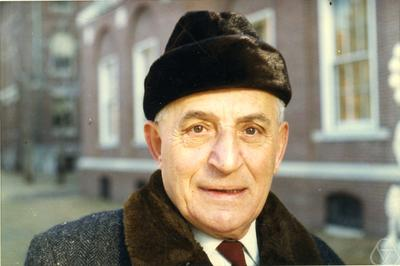
\includegraphics[height=130pt]{OZariski.jpg} \\ \vspace{1em}
	\begin{minipage}{0.7\textwidth}
		\small The $\Bbbk$-vector space $\mathfrak{m}/\mathfrak{m}^2$ is called the \emph{Zariski cotangent space} of $\Spec(R)$, in honor of Oscar Zariski (1899--1986). Picture taken from \href{https://commons.wikimedia.org/wiki/File:Oscar_Zariski.jpg}{Wikimedia Commons}.
	\end{minipage}
\end{figure}

Due to time constraints, we cannot say too much about regular local rings. Below is one of their wonderful properties.
\begin{theorem}\label{prop:regular-local-domain}
	Regular local rings are integral domains.
\end{theorem}
\begin{proof}
	Induction on $d := \dim R$. If $\dim R=0$ then $\mathfrak{m}=\{0\}$, hence $R$ is a field. Assume hereafter that $d > 0$. We know there are only finitely many minimal prime ideals and $\dim_\Bbbk \mathfrak{m}/\mathfrak{m}^2 \geq 1$. By prime avoidance (Proposition \ref{prop:prime-avoidance}) applied to $I := \mathfrak{m}$, the minimal prime ideals and $\mathfrak{m}^2$, there exists $t \in \mathfrak{m} \smallsetminus \mathfrak{m}^2$ that does not lie in any minimal prime ideal. Put $R' := R/(t)$ with maximal ideal $\mathfrak{m}' = \mathfrak{m}/(t)$; our choice of $t$ together with Proposition \ref{prop:system-parameter} imply
	\begin{align*}
		\dim R' & = \dim R - 1, \\
		\dim_\Bbbk \mathfrak{m}'/(\mathfrak{m}')^2 & = \dim_\Bbbk \mathfrak{m}/\mathfrak{m}^2 - 1 = \dim R - 1.
	\end{align*}
	Hence $R'$ is still regular local, and by induction it is a domain. This implies $(t)$ is prime.
	
	Take any minimal prime $\mathfrak{p}$ below $(t)$; note that $t \notin \mathfrak{p}$ by construction. To show $R$ is a domain it suffices to prove $\mathfrak{p}=\{0\}$. Indeed, every $s \in \mathfrak{p}$ can be written as $s=at$, $a \in R$. Since $t \notin \mathfrak{p}$, we must have $a \in \mathfrak{p}$. Hence $\mathfrak{p}=t\mathfrak{p} \subset \mathfrak{m}\mathfrak{p}$. Nakayama's Lemma (Theorem \ref{prop:NAK}) implies $\mathfrak{p} = \{0\}$.
\end{proof}
	% To be compiled by XeLaTeX, preferably under TeX Live.
% LaTeX source for ``Yanqi Lake Lectures on Algebra'' Part III.
% Copyright 2019  李文威 (Wen-Wei Li).
% Permission is granted to copy, distribute and/or modify this
% document under the terms of the Creative Commons
% Attribution-NonCommercial 4.0 International (CC BY-NC 4.0)
% https://creativecommons.org/licenses/by-nc/4.0/

% To be included
\chapter{Dimension of finitely generated algebras}

The main reference is \cite[\S 13]{Mat80}.

\section{Dimensions in fibers}
Consider a homomorphism $\varphi: A \to B$, which induces $\varphi^\sharp: \Spec(B) \to \Spec(A)$ on prime spectra. Given $\mathfrak{p} \in \Spec(A)$, we are interested in the fiber $(\varphi^\sharp)^{-1}(\mathfrak{p})$; the prime ideals $\mathfrak{q}$ therein are described by $\varphi^{-1}(\mathfrak{q}) = \mathfrak{p}$, or equivalently:
\[ \varphi^{-1}(\mathfrak{q}) \cap (A \smallsetminus \mathfrak{p}) = \emptyset, \quad \mathfrak{q} \supset \varphi(\mathfrak{p}). \]
Adopt the convention that a zero ring has $\Spec = \emptyset$. The first condition says that $\mathfrak{q}$ comes from $\Spec(B_{\mathfrak{p}})$, where $B_{\mathfrak{p}}$ is the localization with respect to $\varphi(A \smallsetminus \mathfrak{p})$ (possibly zero). The second condition then says that $\mathfrak{q}B_{\mathfrak{p}}$ lies over the image of $\mathfrak{p}A_{\mathfrak{p}}$. Set
\[ \kappa(\mathfrak{p}) := A_{\mathfrak{p}}/\mathfrak{p}A_{\mathfrak{p}}. \]
The fiber $(\varphi^\sharp)^{-1}(\mathfrak{p})$ is then identified with the spectrum of
\[ B \dotimes{A} \kappa(\mathfrak{p}) = \left( B \dotimes{A} A_{\mathfrak{p}} \right) \dotimes{A_{\mathfrak{p}}} \kappa(\mathfrak{p}) = B_{\mathfrak{p}} \dotimes{A_{\mathfrak{p}}} (A_{\mathfrak{p}}/\mathfrak{p}A_{\mathfrak{p}} ), \]
which is empty if and only if $B \dotimes{A} \kappa(\mathfrak{p})$ is zero. This also equips $(\varphi^\sharp)^{-1}(\mathfrak{p})$ with an extra structure: it is the spectrum of an explicit quotient ring of $B_{\mathfrak{p}}$.

Observe that for all $\mathfrak{q} \in (\varphi^\sharp)^{-1}(\mathfrak{p})$, the localization of $B_{\mathfrak{p}} \dotimes{A_{\mathfrak{p}}} \kappa(\mathfrak{p})$ at the image of $\mathfrak{q}$ is canonically isomorphic to $B_{\mathfrak{q}} \dotimes{A_{\mathfrak{p}}} \kappa(\mathfrak{p})$.

\begin{proposition}\label{prop:fiber-ineq}
	Assume $A, B$ to be Noetherian. Let $\mathfrak{q} \in \Spec(B)$ and $\mathfrak{p} := \varphi^\sharp(\mathfrak{q})$. We have
	\begin{enumerate}[(i)]
		\item $\dim(B_{\mathfrak{q}}) \leq \dim(A_{\mathfrak{p}}) + \dim B_{\mathfrak{q}} \dotimes{A_{\mathfrak{p}}} \kappa(\mathfrak{p})$ (note that the existence of $\mathfrak{q}$ ensures that $B_{\mathfrak{p}} \dotimes{A_{\mathfrak{p}}} \kappa(\mathfrak{p}) \neq \{0\}$, hence $B_{\mathfrak{q}} \dotimes{A_{\mathfrak{p}}} \kappa(\mathfrak{p}) \neq \{0\}$);
		\item equality holds if going-down holds for $\varphi$;
		\item if going-down holds and $\varphi^\sharp$ is surjective, then $\dim(B) \geq \dim(A)$, and for all ideal $\mathfrak{a} \subsetneq A$ we have $\varphi(\mathfrak{a}) B \neq B$ and $\mathrm{ht}(\mathfrak{a}) = \mathrm{ht}(\varphi(\mathfrak{a})B)$.
	\end{enumerate}
\end{proposition}

It is crucial to notice that $\dim B_{\mathfrak{q}} \dotimes{A_{\mathfrak{p}}} \kappa(\mathfrak{p}) = \text{ht}(\mathfrak{q}B_{\mathfrak{q}}/\varphi(\mathfrak{p}) B_{\mathfrak{q}}) = \text{ht}(\mathfrak{q}/\varphi(\mathfrak{p})B)$.

This bounds the source dimension of a morphism by the target dimension plus the fiber dimension, localized both at $\mathfrak{p}$ and $\mathfrak{q} \in (\varphi^\sharp)^{-1}(\mathfrak{p})$. In order to have an equality, a certain submersion-like condition on $\varphi^\sharp$ is evidently required; this explains the going-down condition. Cf. \cite[(6.H)]{Mat80}.

\begin{proof}
	We have an induced local homomorphism $A_{\mathfrak{p}} \to B_{\mathfrak{q}}$ since $\mathfrak{q} \mapsto \mathfrak{p}$. Since (i) and (ii) depend only on this induced homomorphism, we may assume from the outset that $A$, $B$ are local with maximal ideals $\mathfrak{p}, \mathfrak{q}$, and $\varphi$ is a local homomorphism. Let $d := \dim A$ and take a parameter ideal $I = (t_1, \ldots, t_d)$ of $A$, so that $\mathfrak{p}^k \subset I \subset \mathfrak{p}$ for some $k$. It follows that $\sqrt{\varphi(\mathfrak{p}) B} = \sqrt{\varphi(I)B}$, therefore $\dim(B \dotimes{A} \kappa(\mathfrak{p})) = \dim(B/\varphi(\mathfrak{p})B) = \dim (B/\varphi(I)B)$; denote this number as $e$. Take a $s_1, \ldots, s_e \in \mathfrak{q}$ whose images generate a parameter ideal for $B/\varphi(I)B$, and put $J := (\varphi(t_1), \ldots, \varphi(t_d), s_1, \ldots, s_e)$. Then $B/J$ is Artinian, therefore $\dim B \leq d+e$ establishes (i).
	
	As for (ii), we conserve the same hypotheses and take a prime chain $\mathfrak{q} = \mathfrak{q}_0 \supsetneq \cdots \supsetneq \mathfrak{q}_e$ with $\mathfrak{q}_e \supset \varphi(\mathfrak{p})B$ in $B$, as well as a prime chain $\mathfrak{p} = \mathfrak{p}_0 \supsetneq \cdots \supsetneq \mathfrak{p}_d$ in $A$. Note that $\varphi^{-1}(\mathfrak{q}_e) = \mathfrak{p}$ since $e = \dim B/\varphi(\mathfrak{p})B$. By applying going-down repeatedly to the chain $\mathfrak{p}_i$, we obtain a prime chain in $B$
	\[ \mathfrak{q}_e \supsetneq \cdots \supsetneq \mathfrak{q}_{e+d}, \quad \varphi^{-1}(\mathfrak{q}_{e+i}) = \mathfrak{p}_i. \]
	Concatenation with $\mathfrak{q}_0 \supsetneq \cdots$ gives $\dim(B) = d + e$. This shows (ii).
	
	The first assertion of (iii) results from (ii). To show the remaining one, let us show $\varphi(\mathfrak{a})B \neq B$: if $\varphi^\sharp(\mathfrak{q}) = \mathfrak{p} \supset \mathfrak{a}$, then $\mathfrak{q} \supset \varphi(\mathfrak{a}) B$. Next, take a minimal over-prime $\mathfrak{q} \supset \varphi(\mathfrak{a})B$ with $\text{ht}(\mathfrak{q}) = \text{ht}(\varphi(\mathfrak{a})B)$. With $\mathfrak{p} := \varphi^{-1}(\mathfrak{q}) \supset \mathfrak{a}$, we must have $\dim B_{\mathfrak{q}} \otimes \kappa(\mathfrak{p}) = \text{ht}(\mathfrak{q}/\varphi(\mathfrak{p})B) = 0$ by the minimality of $\mathfrak{q}$. An application of (ii) yields
	\begin{gather*}
		\text{ht}(\varphi(\mathfrak{a})B) = \text{ht}(\mathfrak{q}) = \text{ht}(\mathfrak{p}) \geq \text{ht}(\mathfrak{a}).
	\end{gather*}
	To obtain $\leq$, choose $\mathfrak{p} \supset \mathfrak{a}$ with $\text{ht}(\mathfrak{p}) = \text{ht}(\mathfrak{a})$ and take $\mathfrak{q} \in \Spec(B)$ with $\mathfrak{p} = \varphi^{-1}(\mathfrak{q})$; this implies $\mathfrak{q} \supset \varphi(\mathfrak{p})B \supset \varphi(\mathfrak{a})B$. Upon shrinking $\mathfrak{q}$, we may even assume $\mathfrak{q}$ is minimal over $\varphi(\mathfrak{p})B$, i.e. $\text{ht}(\mathfrak{q}/ \varphi(\mathfrak{p})B) = 0$. Using (ii), this entails $\text{ht}(\mathfrak{a}) = \text{ht}(\mathfrak{p}) = \text{ht}(\mathfrak{q}) \geq \text{ht}(\varphi(\mathfrak{a})B)$.
\end{proof}

\vspace{1em}
\begin{center}
	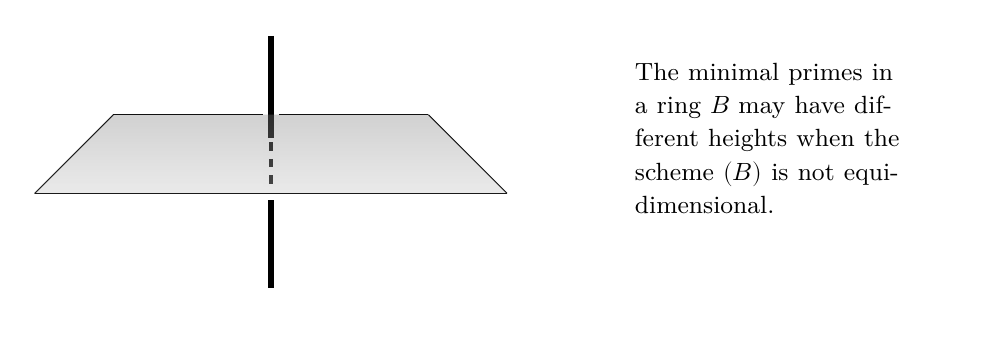
\begin{tikzpicture}
		\draw (-2,1) -- (2,1);
		\draw[line width=6pt, white] (0, 2) -- (0, -1.5);
		\draw[line width=2pt, black] (0,2) -- (0, 0.7);
		\draw[line width=1.5pt, dashed] (0, 0.65) -- (0, 0);
		\draw[line width=2pt, black] (0,0) -- (0, -1.2);
		\draw[line width=5pt, white] (-3,0) -- (3,0);
		\draw (-3,0) -- (3,0);
		\draw (-3,0) -- (-2,1);
		\draw (3,0) -- (2,1);
		\fill[opacity=0.2, shade, color=black!50!white] (-2,1) -- (2,1) -- (3,0) -- (-3,0) -- (-2,1);
		\node[anchor=west, text width=4cm, align=left] at (4.5, 0.7) {\small The minimal primes in a ring $B$ may have different heights when the scheme $\Spec(B)$ is not equi-dimensional.};
	\end{tikzpicture}
\end{center}
\vspace{1em}

Going-down holds for flat $\varphi$ by Theorem \ref{prop:going-down-flat}, therefore the dimension equality
\[ \dim(B_{\mathfrak{q}}) = \dim(A_{\mathfrak{p}}) + \dim B_{\mathfrak{q}} \dotimes{A_{\mathfrak{p}}} \kappa(\mathfrak{p}) \]
holds for flat ring homomorphisms.

\begin{remark}
	In general, if $B$ is a finitely generated algebra over Noetherian $A$ such that $\Spec(B) \to \Spec(A)$ is a closed map, the fiber dimension $\mathfrak{p} \mapsto \dim B/\mathfrak{p}B$ is an \emph{upper semi-continuous function} on the target space $\Spec(A)$. More concretely, the fiber dimension is non-decreasing under specialization of $\mathfrak{p}$. Cf. \cite[\S 14.3]{Eis95} or \cite[(13.E)]{Mat80}. Try to understand this phenomenon intuitively.
\end{remark}

\begin{proposition}\label{prop:dim-integral}
	Suppose $B$ is integral over a subring $A$.
	\begin{enumerate}[(i)]
		\item We have $\dim A = \dim B$.
		\item If we assume moreover that $A, B$ are both Noetherian, then $\mathrm{ht}(\mathfrak{q}) \leq \mathrm{ht}(\mathfrak{q} \cap A)$ for every $\mathfrak{q} \in \Spec(B)$.
		\item Furthermore, if going-down also holds for $A \hookrightarrow B$, we have $\mathrm{ht}(J) = \mathrm{ht}(J \cap A)$ for every ideal $J \subsetneq B$.
	\end{enumerate}
\end{proposition}
\begin{proof}
	Going-up holds and $\Spec(B) \twoheadrightarrow \Spec(A)$ in the situation of (i) by Theorem \ref{prop:Cohen-Seidenberg}, hence $\dim B \geq \dim A$ by lifting prime chains. To prove $\leq$, observe that $\mathfrak{q} \subsetneq \mathfrak{q}'$ implies $\mathfrak{q} \cap A \subsetneq \mathfrak{q}' \cap A$ since there are no inclusion relations in the fibers of $\Spec(B) \to \Spec(A)$.

	As for (ii), note that $\text{ht}(\mathfrak{q}) \leq \text{ht}(\mathfrak{p}) + \text{ht}(\mathfrak{q}/\mathfrak{p}B)$ where $\mathfrak{p} := \mathfrak{q} \cap A$; as the are no inclusion relations in fibers, the last term must be $0$.
	
	Now assume going-down and consider (iii). Take $\mathfrak{q} \in \Spec(B)$ with $\text{ht}(\mathfrak{q}) = \text{ht}(J)$. Put $\mathfrak{p} := \mathfrak{q} \cap A \supset J \cap A$. Again, since there are no inclusions in the fiber over $\mathfrak{p}$ of $\Spec(B) \twoheadrightarrow \Spec(A)$, we have $\dim(B_{\mathfrak{q}}/ \mathfrak{p}B_{\mathfrak{q}}) = 0$. Proposition \ref{prop:fiber-ineq} (ii) implies $\text{ht}(\mathfrak{q})=\text{ht}(\mathfrak{p})$, therefore $\text{ht}(J) \geq \text{ht}(J \cap A)$.
	
	On the other hand, for any $\mathfrak{p} \supset J \cap A$ with $\text{ht}(\mathfrak{p}) = \text{ht}(J \cap A)$, since $A/J \cap A \hookrightarrow B/J$ is integral, there exists $\mathfrak{q} \supset J$ with $\mathfrak{q} \cap A = \mathfrak{p}$. Together with Proposition \ref{prop:fiber-ineq} (i) and $\mathrm{ht}(\mathfrak{q}/\mathfrak{p}B) = 0$, this implies $\text{ht}(J) \leq \text{ht}(\mathfrak{q}) \leq \text{ht}(\mathfrak{p}) = \text{ht}(J \cap A)$ by (ii).
\end{proof}

\section{Calculation for polynomial algebras}
Let us apply the results from the previous section to elucidate the Krull dimension of polynomial algebras.

\begin{theorem}\label{prop:dim-polynomial-alg}
	Let $A$ be a Noetherian ring, we have $\dim A[X_1, \ldots, X_n] = \dim A + n$ for any $n \geq 0$. In particular, $\dim A[X_1, \ldots, X_n] = n$ if $A$ is Artinian (eg.\ a field).
\end{theorem}
\begin{proof}
	Evidently we may assume $n=1$. We shall apply Proposition \ref{prop:fiber-ineq} to $A \hookrightarrow B = A[X]$. Take any $\mathfrak{p} \in \Spec(A)$ and let $\mathfrak{q}$ be a maximal element in $\{\mathfrak{q}' \in \Spec(B): \mathfrak{q} \cap A = \mathfrak{p} \}$. Put $\kappa := \kappa(\mathfrak{p})$. It suffices to show that $B_{\mathfrak{q}} \dotimes{A_{\mathfrak{p}}} \kappa$ has dimension one, since $B$ is free hence flat over $A$, and Proposition \ref{prop:fiber-ineq} will imply
	\[ \dim B_{\mathfrak{q}} = \dim A_{\mathfrak{p}} + 1 \]
	and taking supremum over $\mathfrak{p} \in \Spec(A)$ gives the result.
	
	Indeed, put $B_{\mathfrak{p}} := B[(A \smallsetminus \mathfrak{p})^{-1}] = A_{\mathfrak{p}}[X]$ and $\mathfrak{q}' := \mathfrak{q}[(A \smallsetminus \mathfrak{p})^{-1}] \in \Spec(B_{\mathfrak{p}})$. As $\mathfrak{q}' \supset \mathfrak{p}A_{\mathfrak{p}}$, we have $\overline{\mathfrak{q}'} := \mathfrak{q}' \supset \mathfrak{p}A_{\mathfrak{p}} \in \Spec(\kappa[X])$, and $\overline{\mathfrak{q}'}$ is maximal in the fiber over $\{0\}$ of $\Spec(\kappa[X]) \to \Spec(\kappa)$, i.e.\ in $\MaxSpec(\kappa[X])$. Localization in stages yields
	\[ B_{\mathfrak{q}} \dotimes{A_{\mathfrak{p}}} \kappa \simeq \frac{B_{\mathfrak{q}}}{\mathfrak{p} B_{\mathfrak{q}}} \simeq \left( \frac{B_{\mathfrak{p}}}{ \mathfrak{p} A_{\mathfrak{p}} B_{\mathfrak{p}}} \right)_{\mathfrak{q}' } \simeq \kappa[X]_{\overline{\mathfrak{q}'}}. \]
	As $\kappa[X]$ is a principal ideal domain which is not a field, every maximal ideal thereof has height one. Hence $\dim \kappa[X]_{\overline{\mathfrak{q'}}} = \mathrm{ht}(\mathfrak{q}') = 1$.
\end{proof}

\begin{corollary}\label{prop:poly-alg-ht}
	Let $\Bbbk$ be a field, then for every $0 \leq i \leq n$ we have $\mathrm{ht}(X_1, \ldots, X_i) = i$ in $\Bbbk[X_1, \ldots, X_n]$.
\end{corollary}
\begin{proof}
	The prime chain $\{0\} \subset (X_1) \subsetneq \cdots \subsetneq (X_1, \ldots, X_n)$ has length $n = \dim \Bbbk[X_1, \ldots, X_n]$. Thus for each $0 \leq i \leq n$, the chain $\{0\} \subset (X_1) \subsetneq \cdots \subsetneq (X_1, \ldots, X_i)$ has maximal length among all prime chains starting with $(X_1, \ldots, X_i)$.
\end{proof}

Combined with Theorem \ref{prop:dim-polynomial-alg}, we see that for $\Bbbk$ a field, $R := \Bbbk[X_1, \ldots, X_n]$ and $\mathfrak{p} := (X_1, \ldots, X_i)$, the equality
\[ \text{ht}(\mathfrak{p}) + \dim R/\mathfrak{p} = \dim R. \]
holds. This will be generalized to finitely generated domains over $\Bbbk$.

We record another simple consequence for later use.
\begin{corollary}\label{prop:fg-dimension-bound}
	Let $\Bbbk$ be a field. Any $\Bbbk$-algebra $A$ with $n$ generators has finite dimension $\leq n$.
\end{corollary}
\begin{proof}
	Writing $A = \Bbbk[X_1, \ldots, X_n]/I$ for some ideal $I$, we have $\dim A \leq \Bbbk[X_1, \ldots, X_n]$ since every prime chain in $A$ lifts to $\Bbbk[X_1, \ldots, X_n]$. Now apply Theorem \ref{prop:dim-polynomial-alg}.
\end{proof}

\section{Noether normalization and its consequences}
Fix a field $\Bbbk$. A few preparatory results are in order.

\begin{lemma}\label{prop:normalization-Nagata}
	Suppose $\Bbbk$ is a field and $t \in \Bbbk[X_1, \ldots X_e] \smallsetminus \Bbbk$. There exist $t_1, \ldots, t_{e-1} \in \Bbbk[X_1, \ldots, X_e]$ such that $\Bbbk[X_1, \ldots, X_e]$ is finitely generated as a module over the $\Bbbk$-subalgebra $S := \Bbbk[t_1, \ldots, t_{e-1}, t]$.
\end{lemma}
\begin{proof}
	We seek $t_i$ of the form $X_i - X_e^{k^i}$ where $k$ is a large integer. Then $t$ can be uniquely expressed as a polynomial of $t_1, \ldots, t_{e-1}, X_e$. We claim that upon modifying $t$ by $\Bbbk^\times$, which is clearly harmless, one can choose $k$ such that $t$ is monic as an element of $\Bbbk[t_1, \ldots, t_{e-1}][X_e]$, say of some degree $\delta$. If this is the case,
	\[ t = X_e^\delta + \sum_{0 \leq j < \delta} \left(\text{polynomial in } t_1, \ldots, t_{e-1}\right) X_e^j \]
	says that $X_e$ is integral over $S$, and then $\Bbbk[X_1, \ldots, X_e]$ is generated as an $S$-module by $1, X_e, \ldots, X_e^{\delta-1}$.
	
	To choose $k$, one stares at the expansion
	\[ X_1^{a_1} \cdots X_e^{a_e} = \left(t_1 + X_e^{k^1}\right)^{a_1} \cdots \left(t_{e-1} + X_e^{k^{e-1}}\right)^{a_{e-1}} \cdot X_e^{a_e} = X_e^{a_e + a_1 k^1 + \cdots + a_{e-1} k^{e-1}} + \text{mixed terms}. \]
	If $k > \max\{a_1, \ldots, a_e \}$, the exponent of $X_e$ is simply the base $k$ expression with digits $a_e, a_1, \ldots, a_{e-1}$. Now write $t$ as a linear combination of monomials $X_1^{a_1} \cdots X_e^{a_e}$ and expand them in terms of $t_1, \ldots, t_{e-1}, X_e$. From the observation above, different $(a_1, \ldots, a_e)$ contributes a different exponent of $X_e$ whenever $k \gg 0$. Adjusting $t$ by $\Bbbk^\times$, we get the asserted property.
\end{proof}

\begin{lemma}\label{prop:normalization-aux}
	Let $\mathfrak{a}$ be a nonzero ideal of a domain $R$, then $\dim(R/\mathfrak{a}) + 1 \leq \dim R$.
\end{lemma}
\begin{proof}
	Any prime chain $\mathfrak{p}_0 \supsetneq \cdots \supsetneq \mathfrak{p}_n$ in $R$ with $\mathfrak{p}_n \supset \mathfrak{a}$ can be extended to a prime chain length $n+1$, namely by adjoining $\mathfrak{p}_{n+1} := \{0\}$.
\end{proof}

\begin{theorem}[E.\ Noether, M.\ Nagata]\label{prop:Noether-normalization}\index{Noether normalization}
	Let $B$ be a finitely generated $\Bbbk$-algebra of dimension $n$. Consider a chain of proper ideals $I_1 \subsetneq \cdots \subsetneq I_m$, with $\dim(B/I_j) = d_j$ and $d_1 > \cdots > d_m \geq 0$. Then there exist a $\Bbbk$-subalgebra $A \subset B$ together with an isomorphism $A \simeq \Bbbk[X_1, \ldots, X_n]$, satisfying
	\begin{compactitem}
		\item $B$ is a finitely generated $A$-module, in particular $B$ is integral over $A$;
		\item $I_j \cap A \simeq (X_{d_j+1}, \ldots, X_n)$ under the isomorphism above, for each $1 \leq j \leq m$.
	\end{compactitem}
\end{theorem}

Note that the assumption $I_j \subsetneq I_{j+1}$ is merely for convenience. Allowing $I_j = I_{j+1}$ and $d_j = d_{j+1}$ for some $j$ is surely possible..

\begin{proof}
	Write $B = \Bbbk[Y_1, \ldots, Y_r]/J$, where $r \geq n$ (Corollary \ref{prop:fg-dimension-bound}), and denote the preimage of $I_j$ in $\Bbbk[Y_1, \ldots, Y_r]$ by $\tilde{I}_j$. The first step is to reduce to the case $J=\{0\}$. To see this, we adjoin $\tilde{I}_0 = \{0\}$ (with $d_0 = n$) into the ideal chain; it may happen that $\tilde{I}_0 = \tilde{I}_1$, but that's harmless. Suppose we can find $\tilde{A} \subset \Bbbk[Y_1, \ldots, Y_r]$, $\tilde{A} \simeq \Bbbk[X_1, \ldots, X_r]$ with the required properties relative to $\tilde{I}_\bullet$. Taking quotient by $J$, we obtain the corresponding properties for $I_\bullet$. Indeed, the passage from $\tilde{A}$ to $A := \tilde{A}/(\tilde{A} \cap J)$ truncates the variables $X_{n + 1}, \ldots, X_r$, whereas
	\[ I_j \cap A = \frac{\tilde{I}_j \cap (\tilde{A} + J)}{J} = \frac{(\tilde{I}_j \cap \tilde{A}) + J}{J}  \simeq \frac{\tilde{I}_j \cap \tilde{A}}{J \cap \tilde{A}}; \]
	try to convince yourself of the middle equality.

	Secondly, having reduced to the case $B = \Bbbk[Y_1, \ldots, Y_r]$ (thus $r = n$), it suffices to pick $x_1, \ldots, x_n \in B$ such that
	\begin{enumerate}[(a)]
		\item $B$ is finitely generated as a module over $A := \Bbbk[x_1, \ldots, x_n]$, and
		\item $I_j \cap A \supset (x_{d_j+1}, \ldots, x_n)$ for all $j$.
	\end{enumerate}
	Indeed, (a) implies $\mathrm{Frac}(A)$ and $\mathrm{Frac}(B)$ have the same transcendence degree $n$ over $\Bbbk$, therefore $x_1, \ldots, x_n$ must be algebraically independent over $\Bbbk$. On the other hand, $\dim(B/I_j) = \dim(A/I_j \cap A)$ by (a) and Proposition \ref{prop:dim-integral}; but if $I_j \cap A \supsetneq (x_{d_j+1}, \ldots, x_n)$ then $A/I_j \cap A$ is a proper quotient of the domain $\Bbbk[x_1, \ldots, x_{d_j}]$, therefore would have dimension $< d_j$ by Lemma \ref{prop:normalization-aux}.
	
	We shall construct $x_1, \ldots, x_n$ step by step. Suppose $0 \leq e \leq n$ and that we have produced elements $x'_1, \ldots, x'_e$ and $x_{e+1}, \ldots, x_n$ in $B$ satisfying
	\begin{enumerate}[(i)]
		\item $B$ is finitely generated as a module over $\Bbbk[x'_1, \ldots, x'_e, x_{e+1}, \ldots, x_n] =: S_e$;
		\item $I_j \cap S_e \supset (x_{e+1}, \ldots, x_n)$ when $d_j \leq e$;
		\item $I_j \cap S_e \supset (x_{d_j + 1}, \ldots, x_n)$ when $d_j \geq e$ (with $j = 1, \ldots, m$).
	\end{enumerate}

	For the initial case $e=n$, simply take $x'_i := Y_i$. Our aim is $e=0$. Let us explain the induction step from $e \geq 1$ to $e-1$. The prior argument based on transcendence degrees implies the algebraic independence among
	\[ x'_1, \ldots, x'_e, x_{e+1}, \ldots, x_n. \]
	If $e \leq d_j$ for all $j$, we are done. Otherwise set $j := \min\{j': e > d_{j'} \}$, we contend that
	\[ I_j \cap \Bbbk[x'_1, \ldots, x'_e] \neq \{0\}. \]
	If not, we would have $I_j \cap S_e = (x_{e+1}, \ldots, x_n)$ since $I_j \cap S_e \supset (x_{e+1}, \ldots, x_n)$ by (ii). We have $\dim(S_e/I_j \cap S_e) = \dim(B/I_j) = d_j$ by integrality, whilst $\dim(S_e/(x_{e+1}, \ldots, x_n)) = e$. Contradiction.
	
	Now take $x_e \in I_j \cap \Bbbk[x'_1, \ldots, x'_e] \smallsetminus \{0\}$. Note that $x_e \notin \Bbbk$ as $I_j \neq B$. By Lemma \ref{prop:normalization-Nagata}, we may choose $x''_1, \ldots, x''_{e-1} \in \Bbbk[x'_1, \ldots, x'_e]$ such that $\Bbbk[x'_1, \ldots, x'_e]$ is finitely generated over $\Bbbk[x''_1, \ldots, x''_{e-1}, x_e]$ as a module. It remains to verify that the new sequence
	\[ x''_1, \ldots, x''_{e-1}, x_e, \ldots, x_n \]
	satisfies (i)---(iii) above with $e-1$ replacing $e$.
	
	First, $S_e$ is a finitely generated module over its subalgebra $\Bbbk[x''_1, \ldots, x_n]$ by construction, hence so is $B$ and (i) follows. Next, let $1 \leq j' \leq m$. If $d_{j'} > e-1$, the procedure above does not affect $x_{d_j + 1}, \ldots, x_n$, so they belong to $I_{j'} \cap \Bbbk[x''_1, \ldots, x_n]$. If $d_{j'} < e$, setting $j := \min\{j'' : e > d_{j''} \}$ we have $j' \geq j$ and
	\[ I_{j'} \cap \Bbbk[x''_1, \ldots, x_n] \supset I_j \cap \Bbbk[x''_1, \ldots, x_n] \supset (x_{e+1}, \ldots, x_n) + (x_e). \]
	All in all, we obtain (ii) and (iii).
\end{proof}

\begin{corollary}[Dimension formula]\label{prop:fg-dim-formula}\index{dimension formula}
	Let $B$ be a finitely generated algebra over a field $\Bbbk$. Suppose $B$ is a domain, then for all $\mathfrak{q} \in \Spec(B)$ we have
	\[ \dim(B/\mathfrak{q}) + \mathrm{ht}(\mathfrak{q}) = \dim B. \]
\end{corollary}
\begin{proof}
	Choose a subalgebra $A$ of $B$ as in Theorem \ref{prop:Noether-normalization} and put $\mathfrak{p} = \mathfrak{q} \cap A$. Since $B$ is a domain and $A$ is normal, the Cohen--Seidenberg Theorem \ref{prop:Cohen-Seidenberg} asserts the going-down property for $A \hookrightarrow B$. Proposition \ref{prop:dim-integral} implies that $\dim A = \dim B$, $\dim A/\mathfrak{p} = \dim B/\mathfrak{q}$ and $\text{ht}(\mathfrak{p}) = \text{ht}(\mathfrak{q})$, so we are again reduced to the case $B = \Bbbk[X_1, \ldots, X_n]$ and $\mathfrak{q} = (X_{d+1}, \ldots, X_n)$. This is known by Corollary \ref{prop:poly-alg-ht}.
\end{proof}

The dimension formula allows us to compute $\dim B$ by choosing any prime $\mathfrak{q}$, a prime chain of longest length below $\mathfrak{q}$ (i.e. in $B_{\mathfrak{q}}$) and another one above $\mathfrak{q}$ (i.e. in $B/\mathfrak{q}$); their concatenation will then be a prime chain in $B$ with maximal length $\dim B$. By applying the dimension formula to $\mathfrak{q}, \mathfrak{q}' \subset B$ and to $\mathfrak{q}'/\mathfrak{q} \subset B/\mathfrak{q}$, it follows that $\text{ht}(\mathfrak{q}') = \text{ht}(\mathfrak{q}) + \text{ht}(\mathfrak{q}'/\mathfrak{q})$ for all $\mathfrak{q}' \supsetneq \mathfrak{q}$ in $B$.

For a general Noetherian domain $B$, we call a prime chain \emph{maximal} if it is not properly contained in any prime chain. A priori, a maximal prime chain does not necessarily have length equal to $\dim B$. If
\[ \forall \mathfrak{q}' \supset \mathfrak{q}: \text{primes}, \quad \text{ht}(\mathfrak{q}') = \text{ht}(\mathfrak{q}) + \text{ht}(\mathfrak{q}'/\mathfrak{q}), \]
we say $B$ is a \emph{catenary} domain\index{catenary}. This means that $\text{ht}(\mathfrak{q}'/\mathfrak{q}) = \dim B_{\mathfrak{q}'}/\mathfrak{q}B_{\mathfrak{q}'}$ is the common length of all maximal prime chains between $\mathfrak{q}'$ and $\mathfrak{q}$. In particular, maximal prime chains in $B_{\mathfrak{q}'}$ are automatically longest. As shown above, finitely generated domains over a field are catenary. For a finer analysis of catenary and universally catenary rings, we refer to \cite[\S 14]{Mat80}.

\begin{corollary}
	Suppose $B$ is a domain finitely generated over a field $\Bbbk$. Set $L := \mathrm{Frac}(B)$. Then $\dim B = \mathrm{tr.deg}_\Bbbk(L)$ and it is the common length of maximal prime chains.
\end{corollary}
\begin{proof}
	Choose a subalgebra $A$ of $B$ as in Theorem \ref{prop:Noether-normalization}. Since the field $\text{Frac}(B)$ is a finite extension of $\text{Frac}(A)$ and $\dim A = \dim B$ by Proposition \ref{prop:dim-integral}, the first assertion reduces immediately to the case $B = \Bbbk[X_1, \ldots, X_n]$, which is obvious. As to the second assertion, consider a maximal prime chain $\mathfrak{q}_0 \supsetneq \cdots \supsetneq \mathfrak{q}_n = \{0\}$ in $B$. Maximality implies $\text{ht}(\mathfrak{q}_i/\mathfrak{q}_{i+1}) = 1$ for all $i$ and $\dim B/\mathfrak{q}_0 = 0$. Applying Corollary \ref{prop:fg-dim-formula} repeatedly, we see
	\begin{multline*}
		\dim B = \dim B/\mathfrak{q}_n = \dim B/\mathfrak{q}_{n-1} + \text{ht}(\mathfrak{q}_{n-1}/\mathfrak{q}_n) = \\
		\dim B/\mathfrak{q}_{n-2} + \text{ht}(\mathfrak{q}_{n-1}/\mathfrak{q}_{n-2}) + \text{ht}(\mathfrak{q}_{n-1}/\mathfrak{q}_n) = \cdots = \dim B/\mathfrak{q}_0 + \sum_{i=0}^{n-1} \text{ht}(\mathfrak{q}_i/\mathfrak{q}_{i+1})
	\end{multline*}
	which equals $n$.
\end{proof}

\begin{remark}
	Recall that finitely generated domains over an algebraically closed field $\Bbbk$ are objects ``opposite'' to the irreducible affine $\Bbbk$-varieties. It is instructive to make a comparison with the analytic theory when $\Bbbk=\CC$. Let $\mathcal{X}$ be a compact connected complex manifold of (complex) dimension $n$. Denote by $\mathcal{M}(\mathcal{X})$ the field of meromorphic functions on $\mathcal{X}$. Siegel proved that $\text{tr.deg}_{\CC}(\mathcal{M}(\mathcal{X})) \leq n$. When $\mathcal{X}$ is a projective algebraic $\CC$-variety, equality holds and we have $\mathcal{M}(\mathcal{X}) = \text{Frac}(A)$ if $\Spec(A)$ is any open dense affine subscheme in $\mathcal{X}$. In general, the abundance of meromorphic functions on $\mathcal{X}$ is a subtle issue, cf. the case of Riemann surfaces ($n=1$). Compact connected complex manifolds with $\text{tr.deg}_{\CC}(\mathcal{M}(\mathcal{X})) = \dim_{\CC} \mathcal{X}$ are called \emph{Moishezon manifolds}.\index{Moishezon manifolds}
	
	Non-algebraic Moishezon manifolds do exist, and Moishezon proved that a Moishezon manifold is projective, hence algebraic, if and only if it is Kähler. Following M.\ Artin and D.\ Knutson, one can enlarge the category of $\CC$-schemes into that of \emph{algebraic spaces} over $\CC$, and there is an analytification functor $\mathcal{X} \mapsto \mathcal{X}_{\text{an}}$ that sends algebraic spaces of finite type over $\CC$ to complex analytic varieties. M. Artin \cite[\S 7]{Ar70} showed that the analytification establishes an equivalence between the category of smooth proper algebraic spaces of finite type over $\CC$ and that of Moishezon manifolds. Therefore, such manifolds still retain an algebraic flavor: they are quotients of certain $\CC$-schemes by étale equivalence relations.
\end{remark}

	% To be compiled by XeLaTeX, preferably under TeX Live.
% LaTeX source for ``Yanqi Lake Lectures on Algebra'' Part III.
% Copyright 2019  李文威 (Wen-Wei Li).
% Permission is granted to copy, distribute and/or modify this
% document under the terms of the Creative Commons
% Attribution-NonCommercial 4.0 International (CC BY-NC 4.0)
% https://creativecommons.org/licenses/by-nc/4.0/

% To be included
\chapter{Serre's criterion for normality and depth}

References: \cite[\S 11]{Eis95} and \cite[{X.1}]{Bour98}. Except in the last section, we will try to avoid the use of depth as in \cite{Eis95}.

\section{Review of discrete valuation rings}
Let $R$ be an integral domain.

\begin{definition}\index{discrete valuation ring}
	A \emph{discrete valuation} on a field $K$ is a surjective map $v: K^\times \to \Z$ such that
	\begin{itemize}
		\item $v(xy) = v(x) + v(y)$, and
		\item $v(x+y) \geq \min\{v(x), v(y) \}$
	\end{itemize}
	for all $x,y \in K^\times$, where we set $v(0) = +\infty$ for convenience. We say a domain $R$ with $K := \mathrm{Frac}(R)$ is a \emph{discrete valuation ring}, abbreviated as DVR, if there exists a discrete valuation $v$ such that
	\[ R = v^{-1}([0, +\infty]). \]
	We say $t \in R$ is a \emph{uniformizer} if $v(t)=1$.\index{uniformizer}
\end{definition}
It follows immediately that $R^\times = v^{-1}(0)$. Uniformizers are unique up to $R^\times$. Note that $v(K^\times) = \Z$ implies that $R$ cannot be a field.

\begin{example}
	The ring $\Z_p$ of $p$-adic integers ($p$: prime number) together with the usual $p$-adic valuations are standard examples of DVR. The algebra of formal power series $\Bbbk\llbracket X\rrbracket$ are also DVR: the valuation of $\sum_n a_n X^n$ is the smallest $n$ such that $a_n \neq 0$.
	
	More generally, in the geometric context, discrete valuations can be defined by looking at the vanishing order of rational/meromorphic functions along subvarieties of codimension one with suitable regularities.
\end{example}

\begin{lemma}\label{prop:dvr-regular}
	Let $R$ be a discrete valuation ring with valuation $v$ and uniformizer $t$. Every ideal $\mathfrak{a} \neq \{0\}$ of $R$ has the form $(t^r)$ for a unique $r \geq 0$. In particular, $R$ is a local principal ideal domain which is not a field, hence is of dimension $1$.
\end{lemma}
\begin{proof}
	Take $r := \min\{v(x) : x \in \mathfrak{a} \}$.
\end{proof}

In the exercises below, we assume $R$ is a discrete valuation ring with valuation $v$.
\begin{exercise}
	Show that $t$ is a uniformizer if and only if it generates the maximal ideal of $R$.
\end{exercise}
\begin{exercise}
	Reconstruct $v$ from the ring-theoretic structure of $R$.
\end{exercise}

Recall that a regular local ring $R$ with $\dim R = 1$ is a Noetherian local ring whose maximal ideal $\mathfrak{m}$ is principal and nonzero; elements generating $\mathfrak{m}$ are called the regular parameters for $R$.
\begin{proposition}\label{prop:reg-local-dvr}
	Suppose $t$ is a regular parameter in a regular local ring $R$ of dimension one, then $R$ is a domain, and every element $x \in R \smallsetminus \{0\}$ can be uniquely written as $x = t^r u$ with $r \geq 0$ and $u \in R^\times$. This makes $R$ into a discrete valuation ring by setting $v(x) = r$, for which $t$ is a uniformizer.
	
	Therefore $R$ is a discrete valuation ring. Conversely, every discrete valuation ring is regular local of dimension $1$.
\end{proposition}
\begin{proof}
	From Theorem \ref{prop:regular-local-domain} we know regular local rings are Noetherian domains. By applying Krull's Intersection Theorem (Corollary \ref{prop:Krull-intersection-domain}) to the powers of $(t)$, we see that $r := \sup\{k \geq 0: x \in (t)^k \}$ is finite. Write $x = t^r u$. Since $R^\times = R \smallsetminus \mathfrak{m}$, we see $u \in R^\times$. As to uniqueness, suppose $t^r u = t^s w$ with $r \geq s$, then $t^{r-s} = u^{-1}w \in R^\times$ implies $r=s$, hence $u=w$ as $R$ is a domain. As every element of $\text{Frac}(R)^\times$ is uniquely expressed as $t^r u$ with $r \in \Z$, one readily checks that $v(t^r u) = r$ satisfies all the requirements of discrete valuation.
	
	The converse direction has been addressed in Lemma \ref{prop:dvr-regular}.
\end{proof}

To recap, in dimension one we have
\[ \text{regular local ring} \iff \text{discrete valuation ring}. \]
This will be related to normality later on.

\begin{exercise}
	Explain that the regular local rings of dimension $0$ are just fields.
\end{exercise}

\section{Auxiliary results on the total fraction ring}
Let $R$ be a ring, henceforth assumed Noetherian. If there exist a non zero-divisor $t \in R$ and $\mathfrak{p} \in \text{Ass}(R/(t))$, we say $\mathfrak{p}$ is \emph{associated to a non zero-divisor}.

\begin{lemma}\label{prop:zero-test-ass}
	Let $M$ be a finitely generated $R$-module. An element $x \in M$ is zero if and only if its image in $M_{\mathfrak{p}}$ is zero for every maximal element $\mathfrak{p}$ in $\mathrm{Ass}(M)$.
\end{lemma}
\begin{proof}
	Suppose $x \neq 0$. Since $M$ is Noetherian, among ideals of the form $\text{ann}(y)$ there is a maximal one containing $\text{ann}(x)$, and we have seen in Lemma \ref{prop:Ass-maximal} that such an ideal $\mathfrak{p}$ belongs to $\text{Ass}(M)$. Since $\text{ann}(x) \subset \mathfrak{p}$, we have $x/1 \in M_{\mathfrak{p}} \smallsetminus \{0\}$.
\end{proof}

Call a ring \emph{reduced}\index{reduced ring} if it has no nilpotent element except zero.
\begin{lemma}
	Suppose $R$ is reduced, then $\mathrm{Ass}(R)$ consists of minimal primes.
\end{lemma}
\begin{proof}
	As $R$ is reduced, $\{0\} = \sqrt{0_R}$ is the intersection of minimal prime ideals $\mathfrak{p}_1, \mathfrak{p}_2, \ldots$ (all lying in $\text{Ass}(R)$, hence finite in number). By the theory of primary decompositions, one infers that $\text{Ass}(R) = \{\mathfrak{p}_1, \ldots \}$.
\end{proof}

For the next result, we denote by $T$ the set of non zero-divisors of $R$. Recall that the \emph{total fraction ring} $K(R)$ is $R[T^{-1}]$; this is the largest localization such that $R \to K(R)$ is injective, and $K(R) = \text{Frac}(R)$ when $R$ is a domain. The map $\mathfrak{p} \mapsto \mathfrak{p}K(R)$ sets up an order-preserving bijection $\text{Ass}(R) \rightiso \text{Ass}(K(R))$: indeed, if $\mathfrak{p} \ni t$ for some $t \in T$, then $\mathfrak{p}$ cannot belong to $\text{Ass}(R)$ because the union of $\text{Ass}(R)$ equals $R \smallsetminus T$.

\begin{lemma}\label{prop:K-vs-localization}
	Let $R$ be reduced. Then $K(R) \rightiso \prod_{\mathfrak{p}} K(R/\mathfrak{p})$ as $R$-algebras, where $\mathfrak{p}$ ranges over the minimal prime ideals of $R$. For any multiplicative subset $S \subset R$ there is a canonical isomorphism of $R[S^{-1}]$-algebras
	\begin{align*}
	K(R[S^{-1}]) & \rightiso K(R)[S^{-1}].
	\end{align*}
\end{lemma}
In other words, the formation of total fraction ring commutes with localizations.
\begin{proof}
	Each element in $K(R) = R[T^{-1}]$ is either a zero-divisor or invertible. The set of zero-divisors of $K(R)$ is the union of minimal prime ideals $\mathfrak{p}_i K(R)$ of $K(R)$ (where $\text{Ass}(R) = \{ \mathfrak{p}_1, \ldots, \mathfrak{p}_m\}$ by an earlier discussion), therefore each prime ideal of $K(R)$ must equal some $\mathfrak{p}_i K(R)$, by prime avoidance (Proposition \ref{prop:prime-avoidance}). Hence $\mathfrak{p}_1 K(R), \ldots, \mathfrak{p}_m K(R)$ are also the maximal ideals in $K(R)$, with zero intersection. Chinese Remainder Theorem entails that $K(R) \simeq \prod_{i=1}^m K(R)/\mathfrak{p}_i K(R)$. To conclude the first part, notice that $K(R)/\mathfrak{p}_i K(R) = (R/\mathfrak{p}_i)[T^{-1}]$; this is a field in generated by an isomorphic copy of $R/\mathfrak{p}_i$ since $\mathfrak{p}_i \cap T = \emptyset$, hence equals $\text{Frac}(R/\mathfrak{p}_i)$.
	
	As for the second part, one decomposes $K(R[S^{-1}])$ and $K(R)[S^{-1}]$ by the previous step, noting that
	\begin{compactitem}
		\item $R[S^{-1}]$ is reduced;
		\item $\text{Ass}(R[S^{-1}]) = \left\{ \mathfrak{p}_i R[S^{-1}]: 1 \leq i \leq m, \; \mathfrak{p}_i \cap S = \emptyset \right\}$ consists of minimal primes;
		\item $K\left( R[S^{-1}] \big/ \mathfrak{p}_i R[S^{-1}]\right) \simeq K(R/\mathfrak{p}_i) = K(R/\mathfrak{p}_i)[S^{-1}]$ when $\mathfrak{p}_i \cap S = \emptyset$, by the arguments above;
		\item $K(R/\mathfrak{p}_i)[S^{-1}] = \{0\}$ when $\mathfrak{p}_i \cap S \neq \emptyset$.
	\end{compactitem}
	A term-by-term comparison finishes the proof.
\end{proof}

We use Lemma \ref{prop:K-vs-localization} to interchange $K(\cdot)$ and localizations in what follows.
\begin{lemma}\label{prop:intersection-ass}
	Suppose $R$ is reduced. Then $x \in K(R)$ belongs to $R$ if and only if its image in $K(R)_{\mathfrak{p}} = K(R_{\mathfrak{p}})$ belongs to $R_{\mathfrak{p}}$ for every prime $\mathfrak{p}$ associated to a non zero-divisor.
\end{lemma}
\begin{proof}
	Only the ``if'' direction requires a proof. Write $x = a/t$ with $t$ not a zero-divisor. Suppose that $a \notin (t)$, i.e. $a$ does not map to zero in $R/(t)$. Lemma \ref{prop:zero-test-ass} asserts there exists $\mathfrak{p} \in \text{Ass}(R/(t))$ such that $a$ does not map to $0 \in (R/(t))_{\mathfrak{p}} = R_{\mathfrak{p}}/t R_{\mathfrak{p}}$. It follows that the image of $a/t$ in $K(R_{\mathfrak{p}})$ does not lie in $R_{\mathfrak{p}}$.
\end{proof}

\section{On normality}
Fix a Noetherian ring $R$.

\begin{exercise}
	Suppose $R$ is a domain, $K := \text{Frac}(R)$. If $R = \bigcap_{i \in I} R_i$ where $\{ R_i \subset K\}_{i \in I}$ are subrings such that $\text{Frac}(R_i) = K$ and $R_i$ is normal, for each $i$, then $R$ is normal.
\end{exercise}

\begin{proposition}\label{prop:normality-principal}
	Let $R$ be a Noetherian domain. Then $R$ is normal if and only if for every principal ideal $(t) \subset R$ and every $\mathfrak{p} \in \mathrm{Ass}(R/(t))$, the ideal $\mathfrak{p}R_{\mathfrak{p}}$ is principal.
\end{proposition}
\begin{proof}
	Assume the conditions above. To prove the normality of $R$, it suffices to use $R = \bigcap R_{\mathfrak{p}}$ where $\mathfrak{p}$ ranges over the primes associated to nonzero principal ideals (consequence of Lemma \ref{prop:intersection-ass}). Indeed, each $R_{\mathfrak{p}}$ is regular, hence normal by Proposition \ref{prop:reg-local-dvr}, therefore so is their intersection by the previous exercise.
	
	Conversely, assume $R$ is normal and let $\mathfrak{p} \in \text{Ass}(R/(t))$ with $t \neq 0$, we have to show $\mathfrak{p}R_{\mathfrak{p}}$ is principal. Upon replacing $R$ by $R_{\mathfrak{p}}$ and recalling how associated primes behave under localization, we may even assume $R$ is local with maximal ideal $\mathfrak{p}$. Express $\mathfrak{p}$ as the annihilator of some $\bar{x} \in R/(t)$ with $x \in R$. Define the fractional ideal
	\[ \mathfrak{p}^{-1} := \{ y \in \text{Frac}(R) : y\mathfrak{p} \subset R \}. \]
	It is an $R$-submodule of $\text{Frac}(R)$ containing $R$. Define the $R$-submodule $\mathfrak{p}^{-1}\mathfrak{p}$ of $\text{Frac}(R)$ in the obvious way. Clearly $\mathfrak{p} \subset \mathfrak{p}^{-1}\mathfrak{p} \subset R$. By maximality of $\mathfrak{p}$, exactly one of the $\subset$ is equality. If $\mathfrak{p}\mathfrak{p}^{-1}=\mathfrak{p}$, every element of $\mathfrak{p}^{-1}$ is integral over $R$, hence $\mathfrak{p}^{-1} \subset R$ by normality (integrality is ``witnessed'' by the module $\mathfrak{p}$). From $\mathfrak{p}x \subset (t)$ we see $x/t \in \mathfrak{p}^{-1} = R$; this would imply $\bar{x} = 0$ and $\mathfrak{p}=R$, which is absurd.
	
	Therefore we must have $\mathfrak{p}\mathfrak{p}^{-1} = R$. This implies that $\mathfrak{p}y \not\subset \mathfrak{p}$ for some $y \in \mathfrak{p}^{-1}$, hence $\mathfrak{p}y = R$ since $R$ is local. Hence $\mathfrak{p} = y^{-1}R \simeq R$ is principal.
\end{proof}

\begin{corollary}\label{prop:normality-dvr}
	The following are equivalent for a local domain $R$:
	\begin{enumerate}[(i)]
		\item $R$ is normal of dimension $1$;
		\item $R$ is a regular local ring of dimension $1$;
		\item $R$ is a discrete valuation ring.
	\end{enumerate}
\end{corollary}
\begin{proof}
	(iii) $\implies$ (i). We have seen that discrete valuation rings are principal ideal rings of dimension $1$, therefore also normal by unique factorization property.
	
	(i) $\implies$ (ii). Under the normality assumption, choose any $t \in R \smallsetminus \{0\}$. Since $\dim R = 1$ and $\{0\}$ is a prime ideal, the associated prime of $(t)$ can only be the maximal ideal $\mathfrak{m}$, which is principal by Proposition \ref{prop:normality-principal}. This shows that $R$ is regular local.
	
	(ii) $\implies$ (iii) is included in Proposition \ref{prop:reg-local-dvr}.
\end{proof}

\begin{corollary}
	Let $R$ be a Noetherian normal domain. Then
	\[ R = \bigcap_{\mathrm{ht}(\mathfrak{p}) = 1} R_{\mathfrak{p}} \]
	inside $\mathrm{Frac}(R)$.
\end{corollary}
\begin{proof}
	Evidently $\subset$ holds. By Lemma \ref{prop:intersection-ass} together with Proposition \ref{prop:normality-principal}, $R$ can be written as an intersection of $R_{\mathfrak{p}}$ where $\mathfrak{p}$ is associated to some non zero-divisor, such that $\mathfrak{p}R_{\mathfrak{p}}$ is principal; it suffices to show $\text{ht}(\mathfrak{p})=1$. From $\mathfrak{p} \neq \{0\}$ we see $\text{ht}(\mathfrak{p}) \geq 1$; on the other hand, by Hauptidealsatz or by the discussion on regular local rings, we see $\text{ht}(\mathfrak{p}) = \text{ht}(\mathfrak{p}R_{\mathfrak{p}}) \leq 1$.
\end{proof}

\section{Serre's criterion}

\begin{lemma}\label{prop:reduced-test}
	Let $R$ be a Noetherian ring. Suppose that
	\begin{compactitem}
		\item the primes in $\mathrm{Ass}(R)$ are all minimal, and
		\item $R_{\mathfrak{p}}$ is a field for every minimal prime ideal $\mathfrak{p}$,
	\end{compactitem}
	then $R$ is reduced.
\end{lemma}
\begin{proof}
	Take a minimal primary decomposition $\{0\} = I_1 \cap \cdots \cap I_m$ with $\text{Ass}(R/I_j) = \{\mathfrak{p}_j = \sqrt{I_j} \}$ and $\text{Ass}(R) = \{\mathfrak{p}_1, \ldots, \mathfrak{p}_m \}$. By the properties of primary ideals, $\mathfrak{p}_j = \sqrt{I_j} \supset I_j$ for all $j$. By assumption each $\mathfrak{p}_j$ is minimal, and $R_{\mathfrak{p}_j}$ is a field. From the uniqueness of non-embedded components in primary decompositions, $I_j = \Ker\left[R \to R_{\mathfrak{p}_j}\right]$ is a prime contained in $\mathfrak{p}_j$, hence $I_j = \mathfrak{p}_j$. We deduce that $\{0\} = \bigcap_{j=1}^m \mathfrak{p}_j$, thereby showing $\sqrt{0_R} = \{0\}$.
\end{proof}

\begin{theorem}[J.-P. Serre]\label{prop:Serre-criterion}\index{Serre's criterion}
	A Noetherian ring $R$ is a finite direct product of normal domains if and only if the following two conditions hold.
	\begin{description}
		\item[R1] The localization of $R$ at every prime ideal of height $1$ (resp. $0$) is a discrete valuation ring (resp. a field).
		\item[S2] For every non zero-divisor $t$ of $R$, the primes in $\mathrm{Ass}(R/(t))$ are all of height $1$; the primes in $\mathrm{Ass}(R)$ are all of height $0$.
	\end{description}
\end{theorem}
The condition \textbf{R1} means regularity in codimension $\leq 1$. The condition \textbf{S2} is often rephrased in terms of \emph{depth}, which will be discussed in Proposition \ref{prop:S2}.

\begin{proof}
	We begin with the $\implies$ direction. Suppose $R = R_1 \times \cdots \times R_n$ where each $R_i$ is a normal domain. As is well-known, $\Spec(R) = \bigsqcup_{i=1}^n \Spec(R_i)$ as topological spaces: to be precise, the elements of $\Spec(R)$ take the form $\mathfrak{p} = R_1 \times \cdots \times \mathfrak{p}_i \times \cdots \times R_n$, where $\mathfrak{p}_i \in \Spec(R_i)$. We have
	\[ \text{ht}(\mathfrak{p}) = \text{ht}(\mathfrak{p}_i), \quad R_{\mathfrak{p}} \simeq (R_i)_{\mathfrak{p}_i}. \]
	Furthermore, one easily checks that
	\[ \text{Ass}(R/(t)) = \bigsqcup_{i=1}^n \text{Ass}(R_i/(t_i)), \quad t = (t_1, \ldots, t_n) \in R \]
	compatibly with the description above.
	
	This reduces the verification of \textbf{S2} to the case of normal domains, which is addressed in Proposition \ref{prop:normality-principal}. The condition \textbf{R1} is implied by Corollary \ref{prop:normality-dvr} since normality is preserved under localizations.
	
	Assume conversely \textbf{R1} and \textbf{S2}. They imply the conditions of Lemma \ref{prop:reduced-test}, hence $R$ is reduced. Now for every prime $\mathfrak{p}$ associated to a non zero-divisor, we have $\text{ht}(\mathfrak{p})=1$ and $R_{\mathfrak{p}}$ is a normal domain by \textbf{R1} $\wedge$ \textbf{S2}. By Lemma \ref{prop:intersection-ass} (as $R$ is reduced), $R$ is integrally closed in $K(R)$: indeed, if $x \in K(R)$ is integral over $R$, so is its image in $K(R_{\mathfrak{p}}) = K(R)_{\mathfrak{p}}$ for every $\mathfrak{p}$ as above, therefore lies in $R_{\mathfrak{p}}$. Decompose $K(R) = \prod_{i=1}^m K(R/\mathfrak{p}_i)$ as in Lemma \ref{prop:K-vs-localization}. The idempotents $e_i \in K(R)$ associated to this decomposition are trivially integral over $R$: $e_i^2 - e_i = 0$, hence $e_i \in R$ for all $i$. It follows that $R = Re_1 + \cdots + Re_m \prod_{i=1}^m Re_i \subset K(R)$ and one easily checks that $Re_i = R/\mathfrak{p}_i$.
	
	Finally, since $R$ is integrally closed in $K(R)$, the decomposition above implies $R/\mathfrak{p}_i$ is integrally closed in $K(R/\mathfrak{p}_i)$. All in all, we have written $R$ as a direct product of normal domains.
\end{proof}

\begin{exercise}
	Recall that for an $R$-module $M$, a prime ideal $\mathfrak{p} \in \text{Ass}(M)$ is called \emph{embedded} if $\mathfrak{p}$ is not a minimal element in $\text{Ass}(M)$. Show that for $M=R$, embedded primes are primes in $\text{Ass}(R)$ with height $> 0$. For $M=R/(t)$ where $t$ is not a zero-divisor, embedded primes are primes in $\text{Ass}(R/(t))$ with height $> 1$. Use this to rephrase \textbf{S2} as follows: there are no embedded primes in $\text{Ass}(R/(t))$ ($t$ not a zero-divisor) or in $\text{Ass}(R)$.
\end{exercise}

\begin{exercise}
	Suppose a ring $R$ is isomorphic to a direct product $\prod_{i \in I} R_i$. Show that $R$ is a domain if and only if $|I|=1$ (say $I=\{i_0\}$), and $R_{i_0}$ is a domain.
\end{exercise}

\begin{corollary}
	A Noetherian domain $R$ is normal if and only if \textbf{R1} and \textbf{S2} hold for $R$.
\end{corollary}
\begin{proof}
	Immediate from the previous exercise and Theorem \ref{prop:Serre-criterion}.
\end{proof}

\section{Introduction to depth}
Based on \cite{Bour98}, we give a brief account on the notion of depth. Let $R$ be a ring and $M$ be an $R$-module, $M \neq \{0\}$. Recall the $\Ext$-functors
\[ \Ext^n_R(X,Y) := H^n(R\mathcal{H}\text{om}(X,Y)) = \text{Hom}_{D^+(R\dcate{Mod})}(X, Y[n]). \]

\begin{definition}[Depth of a module]\index{depth}
	Let $I$ be a proper ideal of $R$. We define the \emph{depth} of $M$ relative to $I$ as
	\[ \text{depth}_I(M) := \inf \left\{n \geq 0: \Ext^n_R(R/I, M) \neq 0 \right\} \]
	with values in $\Z_{\geq 0} \sqcup \{+\infty\}$.
\end{definition}

\begin{proposition}\label{prop:depth-zero}
	For $I$, $M$ as above, the following are equivalent:
	\begin{enumerate}[(i)]
		\item $\mathrm{depth}_I(M)=0$;
		\item for all $x \in I$, the homomorphism $M \xrightarrow{x} M$ is not injective;
		\item $\mathrm{Ass}(M) \cap V(I) \neq \emptyset$.
	\end{enumerate}
\end{proposition}
\begin{proof}
	In each case we have $M \neq \{0\}$. If (i) holds, then $M \xrightarrow{x} M$ vanishes on the image of some nonzero $R/I \to M$, hence (ii). If (ii) holds, the union of $\text{Ass}(M)$ will cover $I$, and (iii) follows by prime avoidance. Finally, suppose $\mathfrak{p} \in \text{Ass}(M) \cap V(I)$, there is an embedding $R/\mathfrak{p} \hookrightarrow M$, which yields a non-zero $R/I \to M$.
\end{proof}

\begin{definition}\index{regular sequence}
	A sequence $x_1, \ldots, x_n \in R$ is called an $M$-\emph{regular sequence} of length $n$ if $(x_1, \ldots, x_n)M \subsetneq M$ and
	\[ 0 \to M/(x_1, \ldots, x_{k-1}) \xrightarrow{x_k} M/(x_1, \ldots, x_{k-1}) \]
	is exact for all $1 \leq k \leq n$.
\end{definition}

\begin{lemma}
	Let $M$ be an $R$-module, $x_1, \ldots, x_r$ be an $M$-regular sequence lying in an ideal $I \subsetneq R$. We have $\mathrm{depth}_I(M) = r + \mathrm{depth}_I(M/(x_1, \ldots, x_r)M)$.
\end{lemma}
\begin{proof}
	The case $r=1$ follows by staring at the long exact sequence attached to $0 \to M \xrightarrow{x_1} M \to M/x_1 M \to 0$. The general case follows by induction on $r$.
\end{proof}

\begin{theorem}\label{prop:regular-vs-depth}
	Assume $R$ Noetherian, $M$ finitely generated and $I \subsetneq R$.
	\begin{enumerate}[(i)]
		\item $\mathrm{depth}_I(M)$ is the supremum of the lengths of $M$-regular sequences with elements in $I$.
		\item Suppose $\mathrm{depth}_I(M) < +\infty$. Every $M$-regular sequence with elements in $I$ can be extended to one of length $\mathrm{depth}_I(M)$.
		\item The depth of $M$ relative to $I$ is finite if and only if $V(I) \cap \Supp(M) \neq \emptyset$, or equivalently $IM \neq M$.
	\end{enumerate}
\end{theorem}
\begin{proof}
	To prove (i) and (ii), by the previous Lemma we are reduced to show that $\text{depth}_I(M) > 0$ implies the existence of $x \in I$ which is not a zero-divisor of $M$; this follows from Proposition \ref{prop:depth-zero}.
	
	Now pass to the word ``equivalently'' in (iii). We have $M \neq IM$ if and only if $(M/IM)_{\mathfrak{p}} = M_{\mathfrak{p}}/ I_{\mathfrak{p}} M_{\mathfrak{p}} \neq 0$ for some prime ideal $\mathfrak{p}$. That quotient always vanishes when $\mathfrak{p} \not\supset I$, in which case $I_{\mathfrak{p}} = R_{\mathfrak{p}}$. On the other hand, when $\mathfrak{p} \in V(I)$ we have $I_{\mathfrak{p}} \subset \text{rad}(R_{\mathfrak{p}})$, thus the non-vanishing is equivalent to $M_{\mathfrak{p}} \neq \{0\}$ by Nakayama's Lemma \ref{prop:NAK}.
	
	The ``if'' direction of (iii) is based on the following fact
	\[ IM \neq M \implies \text{depth}_I(M) < +\infty \]
	which will be proved in the next lecture (Theorem \ref{prop:Koszul-depth}) using \emph{Koszul complexes}. As for the ``only if'' direction, $V(I) \cap \Supp(M) = \emptyset$ implies $I + \text{ann}(M) = R$, but the elements in $I + \text{ann}(M)$ annihilate each $\Ext^n(R/I, M)$, hence $\text{depth}_I(M)=+\infty$.
\end{proof}

\begin{figure}[h]
	\centering \vspace{1em} 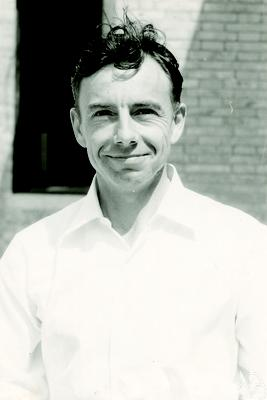
\includegraphics[height=220pt]{Jean-Louis_Koszul.jpg} \\ \vspace{1em}
	\begin{minipage}{0.7\textwidth}
		\small Jean-Louis Koszul (1921---2018) created the Koszul complexes in order to define a cohomology theory for Lie algebras; this device turns out to be a general, convenient construction in homological algebra, which will be discussed in the next lecture. The study of ``Koszulness'' in a broader (eg. operadic) context is now an active area of research. J.-L. Koszul is also a second-generation member of the Bourbaki group. Source: by Konrad Jacobs - \href{http://owpdb.mfo.de/detail?photo_id=2273}{Oberwolfach Photo Collection}, ID 2273.
	\end{minipage}
\end{figure}

\begin{corollary}
	With the same assumptions, let $(x_1, \ldots, x_r)$ be an $M$-regular sequence with $x_i \in I$. It is of length $\mathrm{depth}_I(M)$ if and only if $\mathrm{Ass}(M/(x_1, \ldots, x_r)M) \cap V(I) \neq \emptyset$.
\end{corollary}
\begin{proof}
	The sequence has length $\text{depth}_I(M)$ if and only if $R$-module $M/(x_1, \ldots, x_r)M$ has depth zero, so it remains to apply Proposition \ref{prop:depth-zero}.
\end{proof}

\begin{corollary}
	Let $R$ be a Noetherian local ring with maximal ideal $\mathfrak{m}$, and $M \neq \{0\}$ a finitely generated $R$-module, then $\mathrm{depth}_{\mathfrak{m}}(M) \leq \dim M$.
\end{corollary}
\begin{proof}
	Consider the following situation: $x \in \mathfrak{m}$ is not a zero-divisor for $M \neq \{0\}$. In the discussion of dimensions, we have seen that $d(M) \geq d(M/xM) \geq d(M/xM)-1$, where $d(\cdot)$ is the degree of Hilbert--Samuel polynomial; on the other hand, since the alternating sum of Hilbert--Samuel polynomials in $0 \to M \xrightarrow{x} M \to M/xM \to 0$ has degree $< d(M)$, we infer that $d(M/xM) = d(M) - 1$. Hence $\dim(M/xM) = \dim(M) - 1$. By relating depth to $M$-regular sequences, we deduce $\text{depth}_{\mathfrak{m}}(M) \leq \dim M$.
\end{proof}

\begin{definition}[Cohen--Macaulay modules]\index{Cohen--Macaulay module}
	Let $R$ be a Noetherian ring. A finitely generated $R$-module $M$ is called \emph{Cohen--Macaulay} if
	\[ \mathrm{depth}_{\mathfrak{m}A_{\mathfrak{m}} }(M_{\mathfrak{m}}) = \dim M_{\mathfrak{m}} \]
	for every $\mathfrak{m} \in \MaxSpec(R) \cap \Supp(M)$. We say $R$ is a Cohen--Macaulay ring if it is Cohen--Macaulay as a module.
\end{definition}

\begin{example}
	Regular local rings are Cohen--Macaulay, although we do not prove this here. Another important class of Cohen--Macaulay rings is the algebra of invariants $A^G$ where $A$ is the algebra of regular functions on an affine $\Bbbk$-variety $\mathcal{X}$ with \emph{rational singularities} (eg. $A = \Bbbk[X_1, \ldots, X_n]$) with an action by a reductive $\Bbbk$-group $G$ (finite groups allowed), and we assume $\text{char}(\Bbbk)=0$. Here is the reason: Boutot \cite{Bou87} proved the GIT quotient $\mathcal{X}/\!/G$ has rational singularities as well, hence is Cohen--Macaulay; in characteristic zero this strengthens an earlier theorem of Hochster--Roberts. These algebras are interesting objects from the geometric, algebraic or even combinatorial perspectives.
\end{example}

\begin{exercise}
	Show by using Proposition \ref{prop:depth-zero} that $\text{depth}_{\mathfrak{m}}(R) = 0$ if $R$ is local with maximal ideal $\mathfrak{m}$ and has dimension zero.
\end{exercise}

\begin{proposition}\label{prop:S2}
	The condition \textbf{S2} in Theorem \ref{prop:Serre-criterion} is equivalent to
	\[ \mathrm{ht}(\mathfrak{p}) \geq i \implies \mathrm{depth}_{\mathfrak{p}R_{\mathfrak{p}}}(R_{\mathfrak{p}}) \geq i \]
	for all $\mathfrak{p} \in \Spec(R)$ and $i \in \{1,2\}$.
\end{proposition}
\begin{proof}
	Assume the displayed conditions. We first show that every $\mathfrak{p} \in \text{Ass}(R)$ has height zero. Upon localization we may assume $R$ local with maximal ideal $\mathfrak{p}$, thus $\mathfrak{p}$ has depth zero by Proposition \ref{prop:depth-zero}; our conditions force $\text{ht}(\mathfrak{p})=0$. Next, consider $\mathfrak{p} \in \text{Ass}(R/(t))$ with $t$ non zero-divisor. Note that $t$ remains a non zero-divisor in $R_{\mathfrak{p}}$, and $\mathfrak{p}R_{\mathfrak{p}} \in \text{Ass}(R_{\mathfrak{p}}/(t))$. Hence $\text{depth}(R_{\mathfrak{p}}) = \text{depth}(R_{\mathfrak{p}}/(t)) + 1 = 1$ since $\text{depth}_{\mathfrak{p}}(R_{\mathfrak{p}}/(t)) = 0$ by Proposition \ref{prop:depth-zero}. Our conditions force $\text{ht}(\mathfrak{p}) \leq 1$ and $t \in \mathfrak{p}$ implies $\text{ht}(\mathfrak{p}) > 0$.
	
	Conversely, assume \textbf{S2}. Suppose $\text{ht}(\mathfrak{p}) \geq 1$. If $R_{\mathfrak{p}}$ has depth zero then $\text{Ass}(R_{\mathfrak{p}}) \cap V(\mathfrak{p}R_{\mathfrak{p}}) \neq \emptyset$, which implies $\mathfrak{p}R_{\mathfrak{p}} \in \text{Ass}(R_{\mathfrak{p}})$ thus $\mathfrak{p} \in \text{Ass}(R)$, contradicting \textbf{S2}. Next, suppose $\text{ht}(\mathfrak{p}) \geq 2$. If $R_{\mathfrak{p}}$ has depth $\leq 1$, the standard property
	\[ \forall i \geq 0, \quad \Ext^i_{R_{\mathfrak{p}}}(X_{\mathfrak{p}}, Y_{\mathfrak{p}}) \simeq \Ext^i_R(X,Y)_{\mathfrak{p}} \]
	valid for Noetherian $R$ and finitely generated $R$-modules $X, Y$, yields
	\[ 0 \leq \text{depth}_{\mathfrak{p}}(R) \leq \text{depth}_{\mathfrak{p}R_{\mathfrak{p}}}(R_{\mathfrak{p}}) \leq 1. \]
	If $\text{depth}_{\mathfrak{p}}(R)=0$, there exists of $\mathfrak{p}' \supset \mathfrak{p}$ and $\mathfrak{p}' \in \text{Ass}(R)$ by Proposition \ref{prop:depth-zero}, but \textbf{S2} implies $\text{ht}(\mathfrak{p}) \leq \text{ht}(\mathfrak{p}') = 0$ which is absurd. If $\text{depth}_{\mathfrak{p}}(R)=1$, there exists a non zero-divisor $x$ in $R$ such that $\text{depth}_{\mathfrak{p}}(R/(x)) = 0$. The same argument furnishes $\mathfrak{p}' \supset \mathfrak{p}$ such that $\mathfrak{p}' \in \text{Ass}(R/(x))$. Now \textbf{S2} implies $\text{ht}(\mathfrak{p}) \leq \text{ht}(\mathfrak{p}')=1$, again a contradiction.
\end{proof}

Now the conditions \textbf{R1} and \textbf{S2} can be generalized to arbitrary $k \in \Z_{\geq 0}$:
\begin{description}
	\item[Rk] $\text{ht}(\mathfrak{p}) \leq k$ implies $R_{\mathfrak{p}}$ is a regular local ring, for every $\mathfrak{p} \in \Spec(R)$;
	\item[Sk] $\text{depth}(R_{\mathfrak{p}}) \geq \min\{ k, \text{ht}(\mathfrak{p})\}$ for every $\mathfrak{p} \in \Spec(R)$.
\end{description}
One readily checks their compatibility with Proposition \ref{prop:S2}. Note that \textbf{S0} is trivial, whilst $R$ is Cohen--Macaulay if and only if it satisfies \textbf{Sk} for all $k$.

\begin{example}
	From Theorem \ref{prop:Serre-criterion}, we see that any finite direct product of normal domains of dimension $\leq 2$ is Cohen--Macaulay.
\end{example}

\begin{exercise}
	Show that \textbf{S1} holds if and only if there are no embedded primes in $\text{Ass}(R)$.
\end{exercise}
	% To be compiled by XeLaTeX, preferably under TeX Live.
% LaTeX source for ``Yanqi Lake Lectures on Algebra'' Part III.
% Copyright 2019  李文威 (Wen-Wei Li).
% Permission is granted to copy, distribute and/or modify this
% document under the terms of the Creative Commons
% Attribution-NonCommercial 4.0 International (CC BY-NC 4.0)
% https://creativecommons.org/licenses/by-nc/4.0/

% To be included
\chapter{Some aspects of Koszul complexes}

This lecture is a faithful replay of the relevant sections of \cite{Bour80} and \cite{Bour98}; the main aim here is to complete the proof of Theorem \ref{prop:regular-vs-depth}. In what follows, we work with a chosen ring $R$. We impose no Noetherian or finiteness conditions here.

\section{Preparations in homological algebra}
For any $R$-module $L$, denote its \emph{exterior algebra}\index{exterios algebra} over $R$ by
\[ \bigwedge L := \bigoplus_{n \geq 0} \bigwedge^n L. \]
It is the quotient of the tensor algebra $T(L) = \bigoplus_{n \geq 0} (T^n(L) := L^{\otimes n})$ by the graded ideal generated by the pure tensors
\[ \cdots \otimes x \otimes x \otimes \cdots, \quad x \in L. \]
The multiplication operation in $\bigwedge L$ is written as $\wedge$. Note that $\bigwedge^0 L = T^0(L) = R$ by convention. The traditional notion of exterior algebras encountered in differential geometry is recovered when $\Q \subset R$.

Given $u \in \Hom_R(L, R)$, one can define the corresponding \emph{contractions} $i_u: \bigwedge^{n+1} L \to \bigwedge^n L$, given concretely as
\[ i_u (x_0 \wedge \cdots \wedge x_n) = \sum_{i=0}^n (-1)^i u(x_i) \cdot x_0 \wedge \cdots \widehat{x_i} \cdots \wedge x_n \]
where $\widehat{x_i}$ means $x_i$ is omitted. It is routine to check that $i_u$ satisfies $i_u \circ i_u = 0$, thereby giving rise to a chain complex.

\begin{definition}\label{def:Koszul-general}\index{Koszul complex}
	Let $L$ and $u$ be as above. Define the corresponding \emph{Koszul complex} as $K_\bullet(u) := (\bigwedge^\bullet L, i_u)$. For any $R$-module $M$, put
	\begin{align*}
		K_\bullet(u; M) & := M \dotimes{R} K_\bullet(u), \\
		K^\bullet(u; M) & := \Hom_A(K_\bullet(u), M)
	\end{align*}\index{$K^\bullet(u; M)$}
	which is naturally a chain (resp. cochain) complex in positive degrees; here one regards $M$ as a complex in degree zero. These definitions generalize to the case of any complex $M$, and are functorial in $M$.
\end{definition}

The reader might have encountered the following result in differential geometry.
\begin{proposition}[Homotopy formula]
	For any $x \in L$ and $\omega \in \bigwedge^n L$, we have
	\[ i_u (x \wedge \omega) + x \wedge (i_u(\omega)) = u(x) \omega. \]
\end{proposition}
\begin{proof}
	Consider $\omega = x_1 \wedge \cdots \wedge x_n$. Put $x_0 := x$. The left-hand side equals
	\[ \sum_{i=0}^n (-1)^i \cdot u(x_i) \cdots \wedge \widehat{x_i} \wedge \cdots  \]
	whereas the right-hand side equals
	\[ \sum_{i=1}^n (-1)^{i+1} \cdot u(x_i) x_0 \wedge \cdots \wedge \widehat{x_i} \wedge \cdots. \]
	The terms with a $\widehat{x_i}$ (non-existant --- hopefully this won't generate metaphysical issues) where $i > 0$ cancel out. We are left with $u(x_0) x_1 \wedge \cdots \wedge x_n = u(x) \omega$.
\end{proof}
Obviously, the same formula extends to all $\omega \in \bigwedge L$ by linearity.

\begin{proposition}\label{prop:Koszul-u-vanishing}
	Set $\mathfrak{q} := u(L)$, which is an ideal of $R$. Then $\mathfrak{q}$ annihilates each homology (resp. cohomology) of $K_\bullet(u; M)$ (resp. $K^\bullet(u; M)$). Again, this generalizes to general complexes $M$.
\end{proposition}
\begin{proof}
	Given $t \in \mathfrak{q}$, the homotopy formula implies that the endomorphism $\omega \mapsto t\omega$ of $K_\bullet(u)$ is homotopic to zero, hence so are the induced endomorphisms of $K_\bullet(u; M)$ and $K^\bullet(u; M)$ by standard homological algebra.
\end{proof}

\begin{proposition}\label{prop:Koszul-long-exact-sequence}
	Suppose $L$ is projective over $R$ and $0 \to M' \to M \to M'' \to 0$ is exact. Then there is a natural short exact sequence of complexes
	\[ 0 \to K^\bullet(u; M') \to K^\bullet(u; M) \to K^\bullet(u; M'') \to 0 \]
	which gives rise to a long exact sequence of cohomologies of the Koszul complexes in question.
\end{proposition}
\begin{proof}
	Standard. It suffices to note that $L$ is projective implies each graded piece $\bigwedge^n L$ of $\bigwedge L$ is projective as well.
\end{proof}

\begin{exercise}
	Justify the assertion above concerning the projectivity of $\bigwedge^n L$. Hint: suppose $L$ is a direct summand of a free module $F$, show that $\bigwedge^n L$ is a direct summand of $\bigwedge^n F$ and $\bigwedge^n F$ is free.
\end{exercise}

Similar properties hold for the homological version when $L$ is flat over $R$. One needs the property that $\bigwedge^n L$ is flat if $L$ is.
\begin{exercise}
	Prove the assertion above concerning flatness of $\bigwedge^n L$. Consult the proof in \cite[p.15]{Bour80} if necessary.
\end{exercise}

\section{Auxiliary results on depth}
We fix an ideal $I \subset R$.
\begin{proposition}\label{prop:depth-prod}
	For every family $\{M_\beta\}_{\beta \in \mathcal{B}}$ of $R$-modules, we have
	\[ \mathrm{depth}_I\left(\prod_\beta M_\beta \right) = \inf_\beta \mathrm{depth}_I(M_\beta). \]
\end{proposition}
\begin{proof}
	This follows from $\Ext^n_R(R/I, \prod_i M_i) = \prod_{i \in I} \Ext^n_R(R/I, M_i)$, as is easily seen by taking a projective resolution of $R/I$ and using the fact the $\Hom_R$ preserves direct products in the second variable.
\end{proof}

\begin{remark}
	By stipulation, the empty product is $0$, the zero object of the category $R\dcate{Mod}$. In parallel we define $\inf\emptyset := \infty$, so that Proposition \ref{prop:depth-prod} remains true in this case, since the zero module has infinite depth.
\end{remark}

\begin{proposition}
	Suppose $N$ is an $R$-module annihilated by some $I^m$, where $m \geq 1$. Then $\Ext^i_R(N,M)=0$ whenever $i < \mathrm{depth}_I(M)$.
\end{proposition}
\begin{proof}
	To show $\Ext^i_R(N,M)=0$ for $i < \text{depth}_I(M)$, we begin with the case $m=1$. This case follows by a dimension-shifting argument based on the short exact sequence
	\[ 0 \to K \to (R/I)^{\oplus I} \to M \to 0, \]
	together with induction on $i$ (note that $\Ext^{<0}_R(N,M)=0$ for trivial reasons). The case of general $m$ follows by a standard \emph{dévissage} using
	\[ 0 \to JN \to N \to N/JN \to 0 \]
	and the associated long exact sequence.
\end{proof}

\begin{lemma}\label{prop:depth-power}
	Suppose $J$ is an ideal satisfying $J \supset I^m$ for some $m \geq 1$. Then $\mathrm{depth}_I(M) \leq \mathrm{depth}_J(M)$.
\end{lemma}
\begin{proof}
	From the previous Proposition, we have $\Ext^i_R(R/J, M) = 0$ for $i < \text{depth}_I(M)$ since $I^m$ annihilates $R/J$. The assertion follows upon recalling the definition of depth.
\end{proof}

The following technical results will be invoked in the proof of Theorem \ref{prop:Koszul-depth}.
\begin{proposition}\label{prop:depth-vanishing-aux}
	Let $C^\bullet$ be a cochain complex of $R$-modules such that $n \ll 0 \implies C^n = 0$. Let $h \in \Z$  such that for all integers $n \leq k \leq h$, the depth of $C^n$ with respect to $J_k := \mathrm{ann}(H^k(C^\bullet))$ is $> k-n$, then
	\[ H^{\leq h}(C^\bullet)=0. \]
\end{proposition}
In what follows, we write $H^n = H^n(C^\bullet) = Z^n/B^n$ in the usual notation for homological algebra.
\begin{proof}
	Assume on the contrary that there exists $k \leq h$ with $H^{< k} = 0$ whereas $H^k \neq 0$. Write $J = J_k$. As $J$ annihilates the nonzero $R$-module $H^k$, the criterion of depth-zero modules (Proposition \ref{prop:depth-zero}) implies that $\text{depth}_J(H^k) = 0$. By assumption $\text{depth}_J(C_k) > k-k = 0$, it follows that $\text{depth}_J(Z_k) > 0$ since $Z_k \subset C_k$, by applying the aforementioned criterion of depth-zero. From the short exact sequence
	\[ 0 \to B^k \to Z^k \to H^k \to 0 \]
	we deduce distinguished triangles in $D(R\dcate{Mod})$
	\begin{gather*}
		\mathcal{H}\text{om}(R/J, B^k) \to \mathcal{H}\text{om}(R/J, Z^k) \to \mathcal{H}\text{om}(R/J, H^k) \xrightarrow{+1}, \\
		\mathcal{H}\text{om}(R/J, H^k)[-1] \to \mathcal{H}\text{om}(R/J, B^k) \to \mathcal{H}\text{om}(R/J, Z^k) \xrightarrow{+1}.
	\end{gather*}
	As the leftmost and rightmost terms of the last line are in $D^{\geq 1}(R\dcate{Mod})$, we see
	\[ \text{depth}_J(B^k) \geq 1; \]
	moreover, the piece $\Ext_R^0(R/J, Z^k) \to \Ext_R^0(R/J, H^k) \to \Ext_R^1(R/J, B^k)$ from the long exact sequence shows that $\text{depth}_J(B^k) = 1$. Now for $n < k$ we have short exact sequences
	\[ 0 \to \underbracket{B^n}_{= Z^n} \to C^n \to B^{n+1} \to 0. \]
	Again, one infers from the distinguished triangle
	\[ \mathcal{H}\text{om}(R/J, B^{n+1})[-1] \to \mathcal{H}\text{om}(R/J, B^n) \to \mathcal{H}\text{om}(R/J, C^n) \xrightarrow{+1} , \]
	the assumption $\text{depth}_J(C^n) > k-n$ and descending induction on $n$ that $n < k \implies \text{depth}_J(B_n) = k-n+1$. This is impossible since $B_{\ll 0} = 0$ has infinite depth.
\end{proof}

\begin{corollary}\label{prop:depth-vanishing}
	Let $I \subset R$ be an ideal, $C^\bullet$ be a cochain complex with $n \ll 0 \implies C_n=0$, and $h \in \Z$. Suppose that $n \leq h$ implies $I \cdot H^n(C^\bullet) = 0$ and $\mathrm{depth}_I(C^n) > h-n$. Then $H^{\leq h}(C^\bullet) = 0$.
\end{corollary}
\begin{proof}
	For $k \leq h$ we have $J_k := \text{ann}(H^k(C^\bullet)) \supset I$. Hence Lemma \ref{prop:depth-power} entails that
	\[ n \leq k \leq h \implies \text{depth}_{J_k}(C^n) \geq \text{depth}_I(C^n) > h-n \geq k-n. \]
	Now apply Proposition \ref{prop:depth-vanishing-aux}.
\end{proof}

\section{Koszul complexes and depth}
The simplest Koszul complexes are defined as follows. Given $x \in R$, we form the cochain complex in degrees $\{0,1\}$
\[ K(x) := \left[ R \xrightarrow{x} R \right]. \]
More generally, for any $R$-module $M$, viewed as a complex concentrated in degree zero, and a family $\mathbf{x} = (x_\alpha)_{\alpha \in \mathcal{A}}$ of element of $R$, we define the associated \emph{Koszul complex}\index{Koszul complex} as
\[ K^\bullet(\mathbf{x}; M) := K^\bullet(u; M), \]
where we take $u: R^{\oplus \mathcal{A}} \to R$ corresponding to $\mathbf{x}$ in Definition \ref{def:Koszul-general}. Unfolding definitions, we have \index{$K^\bullet(\mathbf{x};M)$}
\[ K^h(\mathbf{x}; M) = \begin{cases}
	\Hom_R\left( \bigwedge^h (R^{\oplus \mathcal{A}}), M \right), & h \geq 0 \\
	0, & h < 0. 
\end{cases} \]
Therefore $K^h(\mathbf{x}; M)$ consists of families $m(\alpha_1, \ldots, \alpha_h) \in M$ that are alternating in the variables $\alpha_1, \ldots, \alpha_h \in \mathcal{A}$. The differential is
\begin{align*}
	\partial^h: K^h(\mathbf{x}; M) & \longrightarrow K^{h+1}(\mathbf{x}; M) \\
	m & \longmapsto \left[ (\alpha_0, \ldots, \alpha_h) \mapsto \sum_{j=0}^h (-1)^j x_{\alpha_j} \cdot m(\ldots, \widehat{\alpha_j}, \ldots) \right].
\end{align*}
We shall abbreviate the cohomologies of $K^\bullet(\mathbf{x}; M)$ as the \emph{Koszul cohomologies}.

When $\mathcal{A} = \{1, \ldots, n\}$ we revert to
\[ K^\bullet(x_1, \ldots, x_n; M) := M \otimes K(x_1) \otimes \cdots \otimes K(x_n) \]
with the well-known sign convention. Also note that $R^{\oplus \mathcal{A}}$ is projective, hence the Proposition \ref{prop:Koszul-long-exact-sequence} can always be applied to Koszul cohomologies.

Let $I$ denote the ideal generated by $\{x_\alpha: \alpha \in \mathcal{A} \}$. The reader is invited to verify that
\begin{itemize}
	\item $K^\bullet\left( \mathbf{x}, \prod_{\beta \in \mathcal{B}} M_\beta \right) = \prod_{\beta \in \mathcal{B}} K^\bullet(\mathbf{x}; M_\beta)$ for any family $\{M_\beta\}_{\beta \in \mathcal{B}}$ of $R$-modules, and same for their cohomologies;
	\item the $0$-th cohomology of $K^\bullet(\mathbf{x}; M)$ is $\Hom_R(R/I, M) = \{x \in M: Ix=0 \}$, the $I$-torsion part of $M$;
	\item if $|A| = n$, the $n$-th cohomology of $K^\bullet(\mathbf{x}; M)$ is $M/IM$.
\end{itemize}
These facts will cast in our later arguments.

\begin{lemma}\label{prop:Koszul-coho-ann}
	Each cohomology of $K^\bullet(\mathbf{x}; M)$ is annihilated by $I$.
\end{lemma}
\begin{proof}
	Apply Proposition \ref{prop:Koszul-u-vanishing} by observing that $\mathfrak{q} = I$ in our setting.
\end{proof}

\begin{theorem}\label{prop:Koszul-depth}\index{depth}
	Let $M$ be an $R$-module and $\mathbf{x} = \{x_\alpha \}_{\alpha \in \mathcal{A}}$ be a family of elements of $R$, which generate an ideal $I$ of $A$. Then $\mathrm{depth}_I(M)$ equals
	\[ \inf \left\{n \geq 0: H^n(K^\bullet(\mathbf{x}; M)) \neq 0 \right\} \in \Z_{\geq 0} \sqcup \{\infty \} . \]
	Consequently, if $I \subset R$ is an ideal generated by elements $x_1, \ldots, x_n$ and $IM \neq M$, then we have
	\[ \mathrm{depth}_I(M) \leq n. \]
\end{theorem}
\begin{proof}
	Let $d := \text{depth}_I(M)$. Since $K^h(\mathbf{x}; M)$ is a direct product of copies of $M$ (possibly the empty product $=0$), by Proposition \ref{prop:depth-prod} its depth equals either $d$ or $\infty$. Combining Lemma \ref{prop:Koszul-coho-ann} and Corollary \ref{prop:depth-vanishing} (with $h = d-1$), we see that $H^{< d}(K^\bullet(\mathbf{x}; M)) = 0$. It remains to show $H^d(K^\bullet(\mathbf{x}; M)) \neq 0$ provided that $d < \infty$, which we assume from now onwards.

	The case $d=0$ is clear since there exists $\mathfrak{p} \in \text{Ass}(M) \cap V(I)$, therefore $R/\mathfrak{p} \hookrightarrow M$ and $\exists x \in M$ with $\mathfrak{p} x \supset Ix = \{0\}$, whence $H^0(K^\bullet(\mathbf{x}; M)) \neq 0$. Now suppose $d \in \Z_{\geq 1}$ and assume $H^d(K^\bullet(\mathbf{x}; M)) = 0$. Take a free resolution $F_\bullet \to R/I \to 0$ and put $C^\bullet := \Hom_R(F_\bullet, M)$, so that
	\[ H^i(C^\bullet) \simeq \Ext^i_R(R/I, M), \quad i \geq 0. \]
	Hence for $i < d$ we have short exact sequences
	\[ 0 \to B^i \to C^i \to B^{i+1} \to 0 \]
	as usual; recall $B^i, Z^i \subset C^i$. Note that each $C^i$ is a direct product of copies of $M$, hence $H^{\leq d}(K^\bullet(\mathbf{x}; C^i)) = 0$. Indeed, $H^{< d}(K^\bullet(\mathbf{x}; M))=0$ has been settled in the first step, whilst $H^d(K^\bullet(\mathbf{x}; M))$ is the hypothesis to be refuted. It then follows from the long exact sequence for Koszul cohomologies (Proposition \ref{prop:Koszul-long-exact-sequence}) that
	\[ (s \leq d) \wedge (i < d) \implies H^s(K^\bullet(\mathbf{x}; B^{i+1})) \hookrightarrow H^{s+1}(K^\bullet(\mathbf{x}; B^i)). \]
	Suppose $i < d$. As $B^0 = 0$, an iteration yields
	\[ H^{d-i}(K^\bullet(\mathbf{x}; B^{i+1})) \hookrightarrow \cdots \hookrightarrow H^{d+1}(K^\bullet(\mathbf{x}; B^0)) = 0. \]
	In particular, $i=d-1$ gives rise to $H^1(K^\bullet(\mathbf{x}; B^d)) = 0$. Hence the short exact sequence $0 \to B^d \to Z^d \to H^d \to 0$ (for $C^\bullet$) together with Proposition \ref{prop:Koszul-long-exact-sequence} give rise to
	\[ H^0(K^\bullet(\mathbf{x}; Z^d)) \twoheadrightarrow H^0(K^\bullet(\mathbf{x}; H^d)). \]
	As $H^d := H^d(C^\bullet) \simeq \Ext^d_R(R/I, M)$ is nonzero and annihilated by $I$, the right-hand side is nonzero. Hence $H^0(K^\bullet(\mathbf{x}; Z^d)) \neq 0$ and then $H^0(K^\bullet(\mathbf{x}; C^d)) \neq 0$, as the zeroth Koszul cohomology is nothing but the $I$-torsion part.
	
	Finally, recall that $C^d \neq \{0\}$ is a direct product of copies of $M$, consequently
	\[ H^0(K^\bullet(\mathbf{x}; M)) \neq 0. \]
	However, this contradicts the earlier result that $H^{<d}(K^\bullet(\mathbf{x}; M))=0$ since $d \geq 1$.
\end{proof}

This yields an alternative characterization of depth. It also completes the proof of Theorem \ref{prop:regular-vs-depth} as promised in the previous lecture.

% Finalizing...
\vfill
\begin{figure}[h]
	\centering 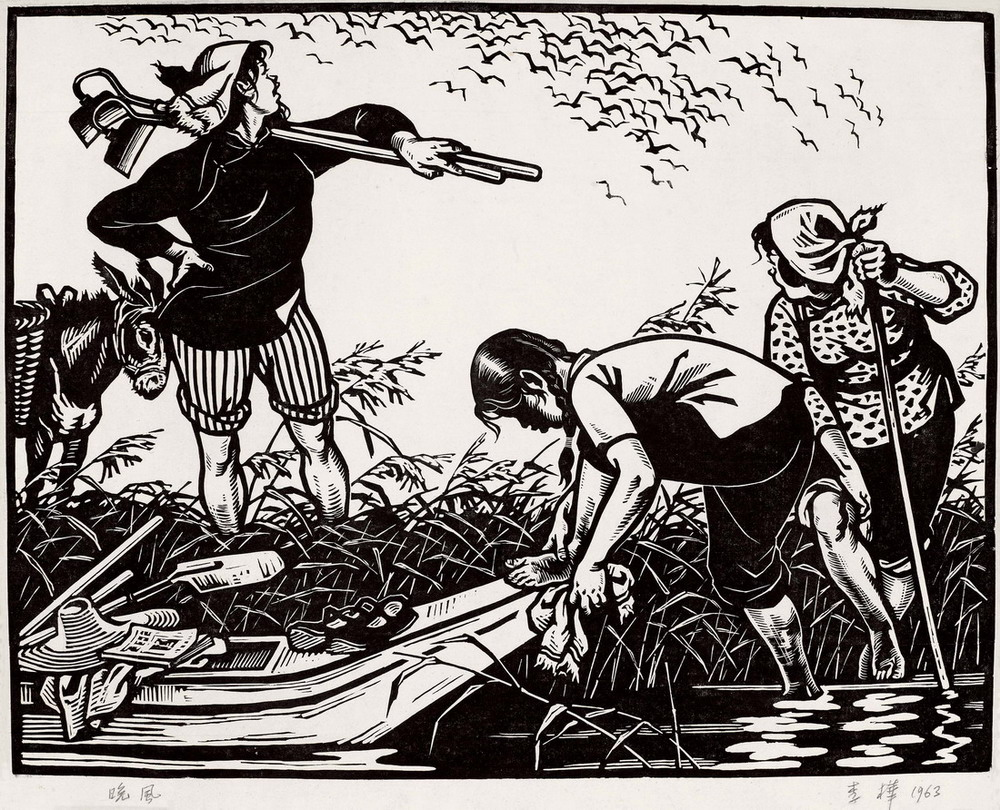
\includegraphics[height=200pt]{WanFeng.jpg} \\ \vspace{1em}
	\begin{minipage}{0.7\textwidth}\begin{center}
			\small \fontspec{Noto Serif CJK SC} 《晚风》, 李桦, 木刻版画, 1963 年.
	\end{center}\end{minipage}
\end{figure}
\vfill

	\backmatter
	\printbibliography[heading=bibintoc]	% For Biber
	\printindex

\end{document}
